\input{../style/preamble}
\input{../latex-math/basic-math}
\input{../latex-math/basic-ml}
\input{../latex-math/ml-nn}

\newcommand{\titlefigure}{figure/rosenblatt_perceptron.jpg}
\newcommand{\learninggoals}{
  \item Historical development of neural networks, from early threshold units to modern foundation models
  \item The single neuron (perceptron) as an affine transformation plus non-linear activation, its hypothesis space, and typical loss functions
  \item Single- and multi-hidden-layer feedforward networks, representation learning, and common activation functions
  \item Compact vector/matrix notation for feedforward network computations
  \item Softmax output layers and loss functions for multi-class classification
  \item The universal approximation theorem and its implications for model flexibility
}

\title{Advanced Artificial Intelligence and Machine Learning}
\date{}

\begin{document}

\lecturechapter{DL Intro I}
\lecture{Advanced AI \& ML}
%%%%%%%%%%%%%%%%%%%%%%%%%%%%%%%%%%%%%%%%%%%%%%%%%%%%%%%%%%%%%%%%%%

\section{Brief History}
%%%%%%%%%%%%%%%%%%%%%%%%%%%%%%%%%%%%%%%%%%%%%%%%%%%%%%%%%%%%%%%%%%

\begin{vbframe}{A Brief History: What Was Possible}
\begin{itemize}
\item \pkg{1943:} McCulloch \& Pitts propose the \enquote{Threshold Logic Unit (TLU)}, the first artificial neuron: binary inputs, a fixed threshold $\theta$, non-adjustable weights.
\vspace{2mm}
\item \pkg{1957:} Rosenblatt's Perceptron generalizes this with real-valued inputs and, crucially, \textbf{learnable} weights.
\vspace{2mm}
\item \pkg{1960:} Widrow \& Hoff's ADALINE learns by adjusting weights based on the weighted sum of the inputs.
\vspace{2mm}
\item \pkg{1965:} Ivakhnenko's Group Method of Data Handling (GMDH) gives the first learning algorithm for supervised, deep, multilayer feedforward networks.
\vspace{2mm}
\item \pkg{1985:} Rumelhart, Hinton \& Williams popularize \textbf{backpropagation} for multilayer perceptrons: efficient gradient computation through composite functions (first derived by Linnainmaa already in 1970 -- more on this in a later session).
\end{itemize}
\begin{figure}
\centering
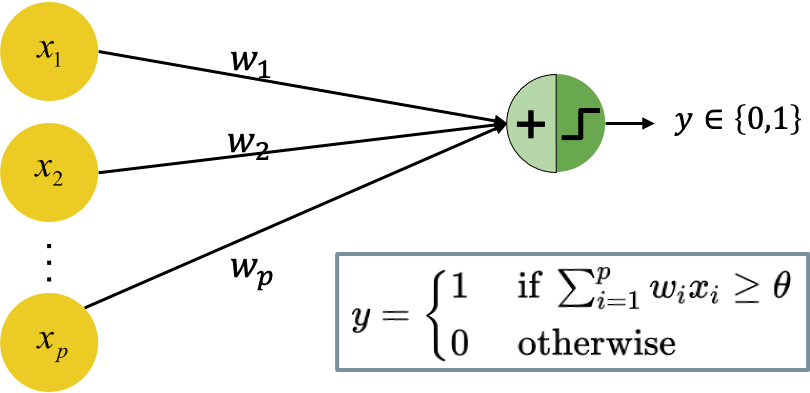
\includegraphics[width=5.5cm]{figure/perceptron_new.png}
\end{figure}
\end{vbframe}
%%%%%%%%%%%%%%%%%%%%%%%%%%%%%%%%%%%%%%%%%%%%%%%%%%%%%%%%%%%%%%%%%%

\begin{vbframe}{A Brief History: Why the Winters}
\begin{itemize}
\item \pkg{1969 --- First AI Winter:} Minsky \& Papert prove that a single perceptron cannot solve the XOR problem: it is not linearly separable (we return to this in detail later). Funding dries up, research stalls.
\vspace{4mm}
\item \pkg{1985 --- Second AI Winter:} Despite backpropagation, expectations outpace results. Kernel machines and graphical models match or beat early neural nets on many tasks, and modeling long sequences remains a fundamental difficulty. \enquote{AI} becomes associated with pseudoscience; investment collapses again.
\end{itemize}
\begin{figure}
\centering
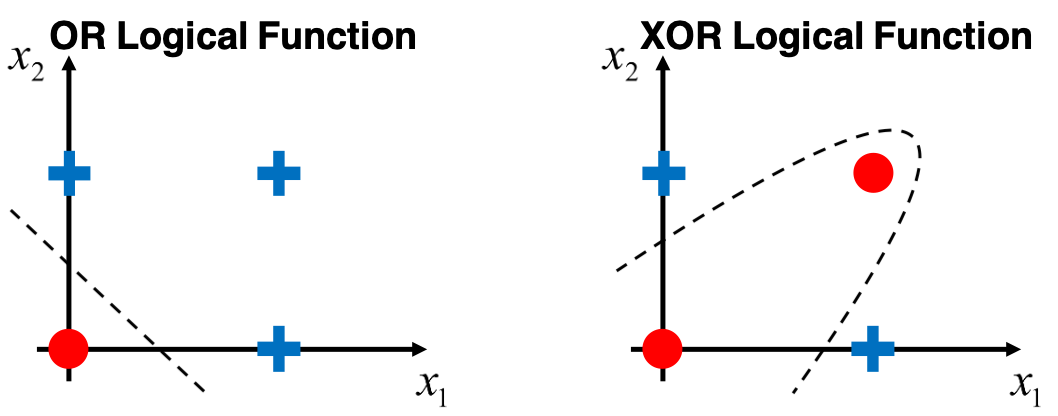
\includegraphics[width=6cm]{figure/orvsxor.png}
\caption{\small The XOR problem: not linearly separable.}
\end{figure}
\end{vbframe}
%%%%%%%%%%%%%%%%%%%%%%%%%%%%%%%%%%%%%%%%%%%%%%%%%%%%%%%%%%%%%%%%%%

\begin{vbframe}{A brief history of neural networks}
\begin{itemize}
\item \pkg{2006:} Age of deep neural networks began.

\begin{itemize}
\footnotesize\item Geoffrey Hinton showed that a deep belief network could be efficiently trained using \textit{greedy layer-wise pretraining}.
\footnotesize\item This wave of research popularized the use of the term deep learning to emphasize that researchers were now able to train deeper neural networks than had been possible before.
\footnotesize\item At this time, deep neural networks outperformed competing AI systems based on other ML technologies as well as hand-designed functionality.
\end{itemize}
\begin{figure}
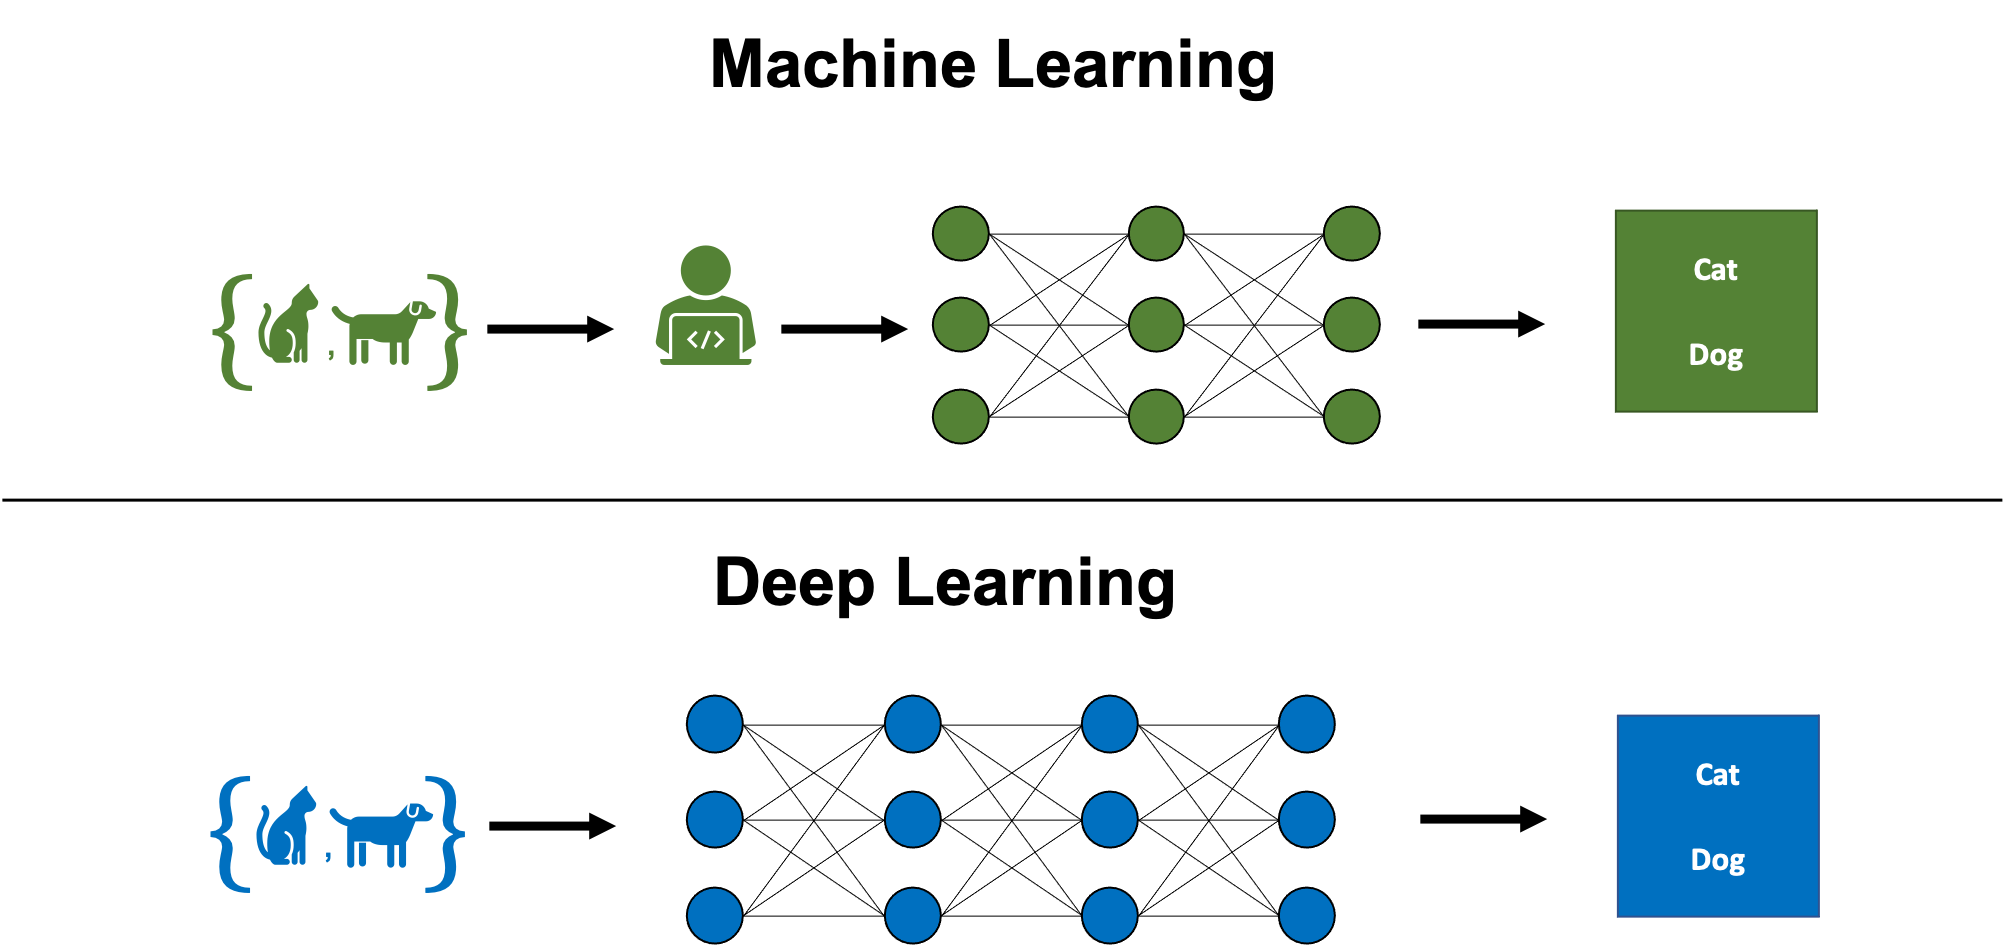
\includegraphics[width=9cm]{figure/dl_feature2.png}

\end{figure}
\end{itemize}
\framebreak
%%%%%%%%%%%%%%%%%%%%%%%%%%%%%%%%%%%%%%%%%%%%%%%%%%%%%%%%%%%%%%%%%%

%\textbf{Why now and not earlier?}
%\begin{enumerate}
%\vspace{2mm}
%\item Significantly bigger datasets.
%\vspace{2mm}
%\item Better algorithms resolving the vanishing gradient problem.
%\vspace{2mm}
%\item Better regularization.
%\vspace{2mm}
%\item Unsupervised representation learning.
%\vspace{2mm}
%\item More layers lead to a significant increase of parameters.
%\vspace{2mm}
%\item Deep neural networks are trained on GPUs, rather than CPUs. So processing power can handle huge amounts of parameters.
%\vspace{2mm}
%\item Investment by industries and universities.
%\vspace{2mm}
%\item DL tools make learning and applying DL easier.
%\end{enumerate}
%\framebreak
%%%%%%%%%%%%%%%%%%%%%%%%%%%%%%%%%%%%%%%%%%%%%%%%%%%%%%%%%%%%%%%%%%

\begin{figure}
\centering
\scalebox{1.1}{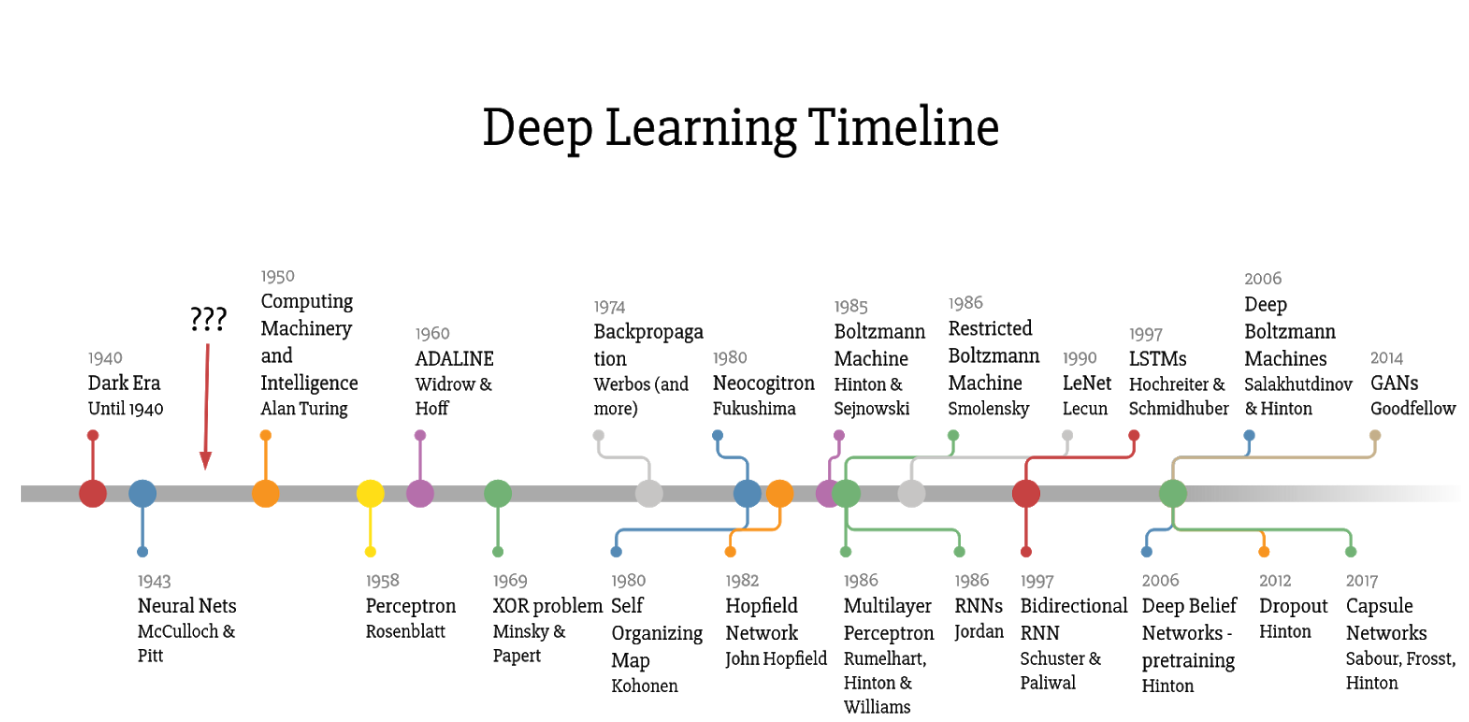
\includegraphics{figure/dl_timeline.png}}
\vspace{.5cm}
\caption{(Vazquez, 2018)}
\framebreak
%%%%%%%%%%%%%%%%%%%%%%%%%%%%%%%%%%%%%%%%%%%%%%%%%%%%%%%%%%%%%%%%%%

\scalebox{1.1}{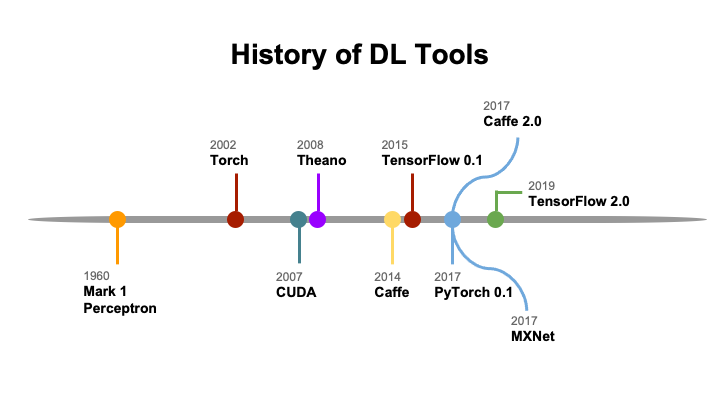
\includegraphics{figure/DL_tools.png}}
\end{figure}
\framebreak
%%%%%%%%%%%%%%%%%%%%%%%%%%%%%%%%%%%%%%%%%%%%%%%%%%%%%%%%%%%%%%%%%%

%\begin{figure}
%\centering
%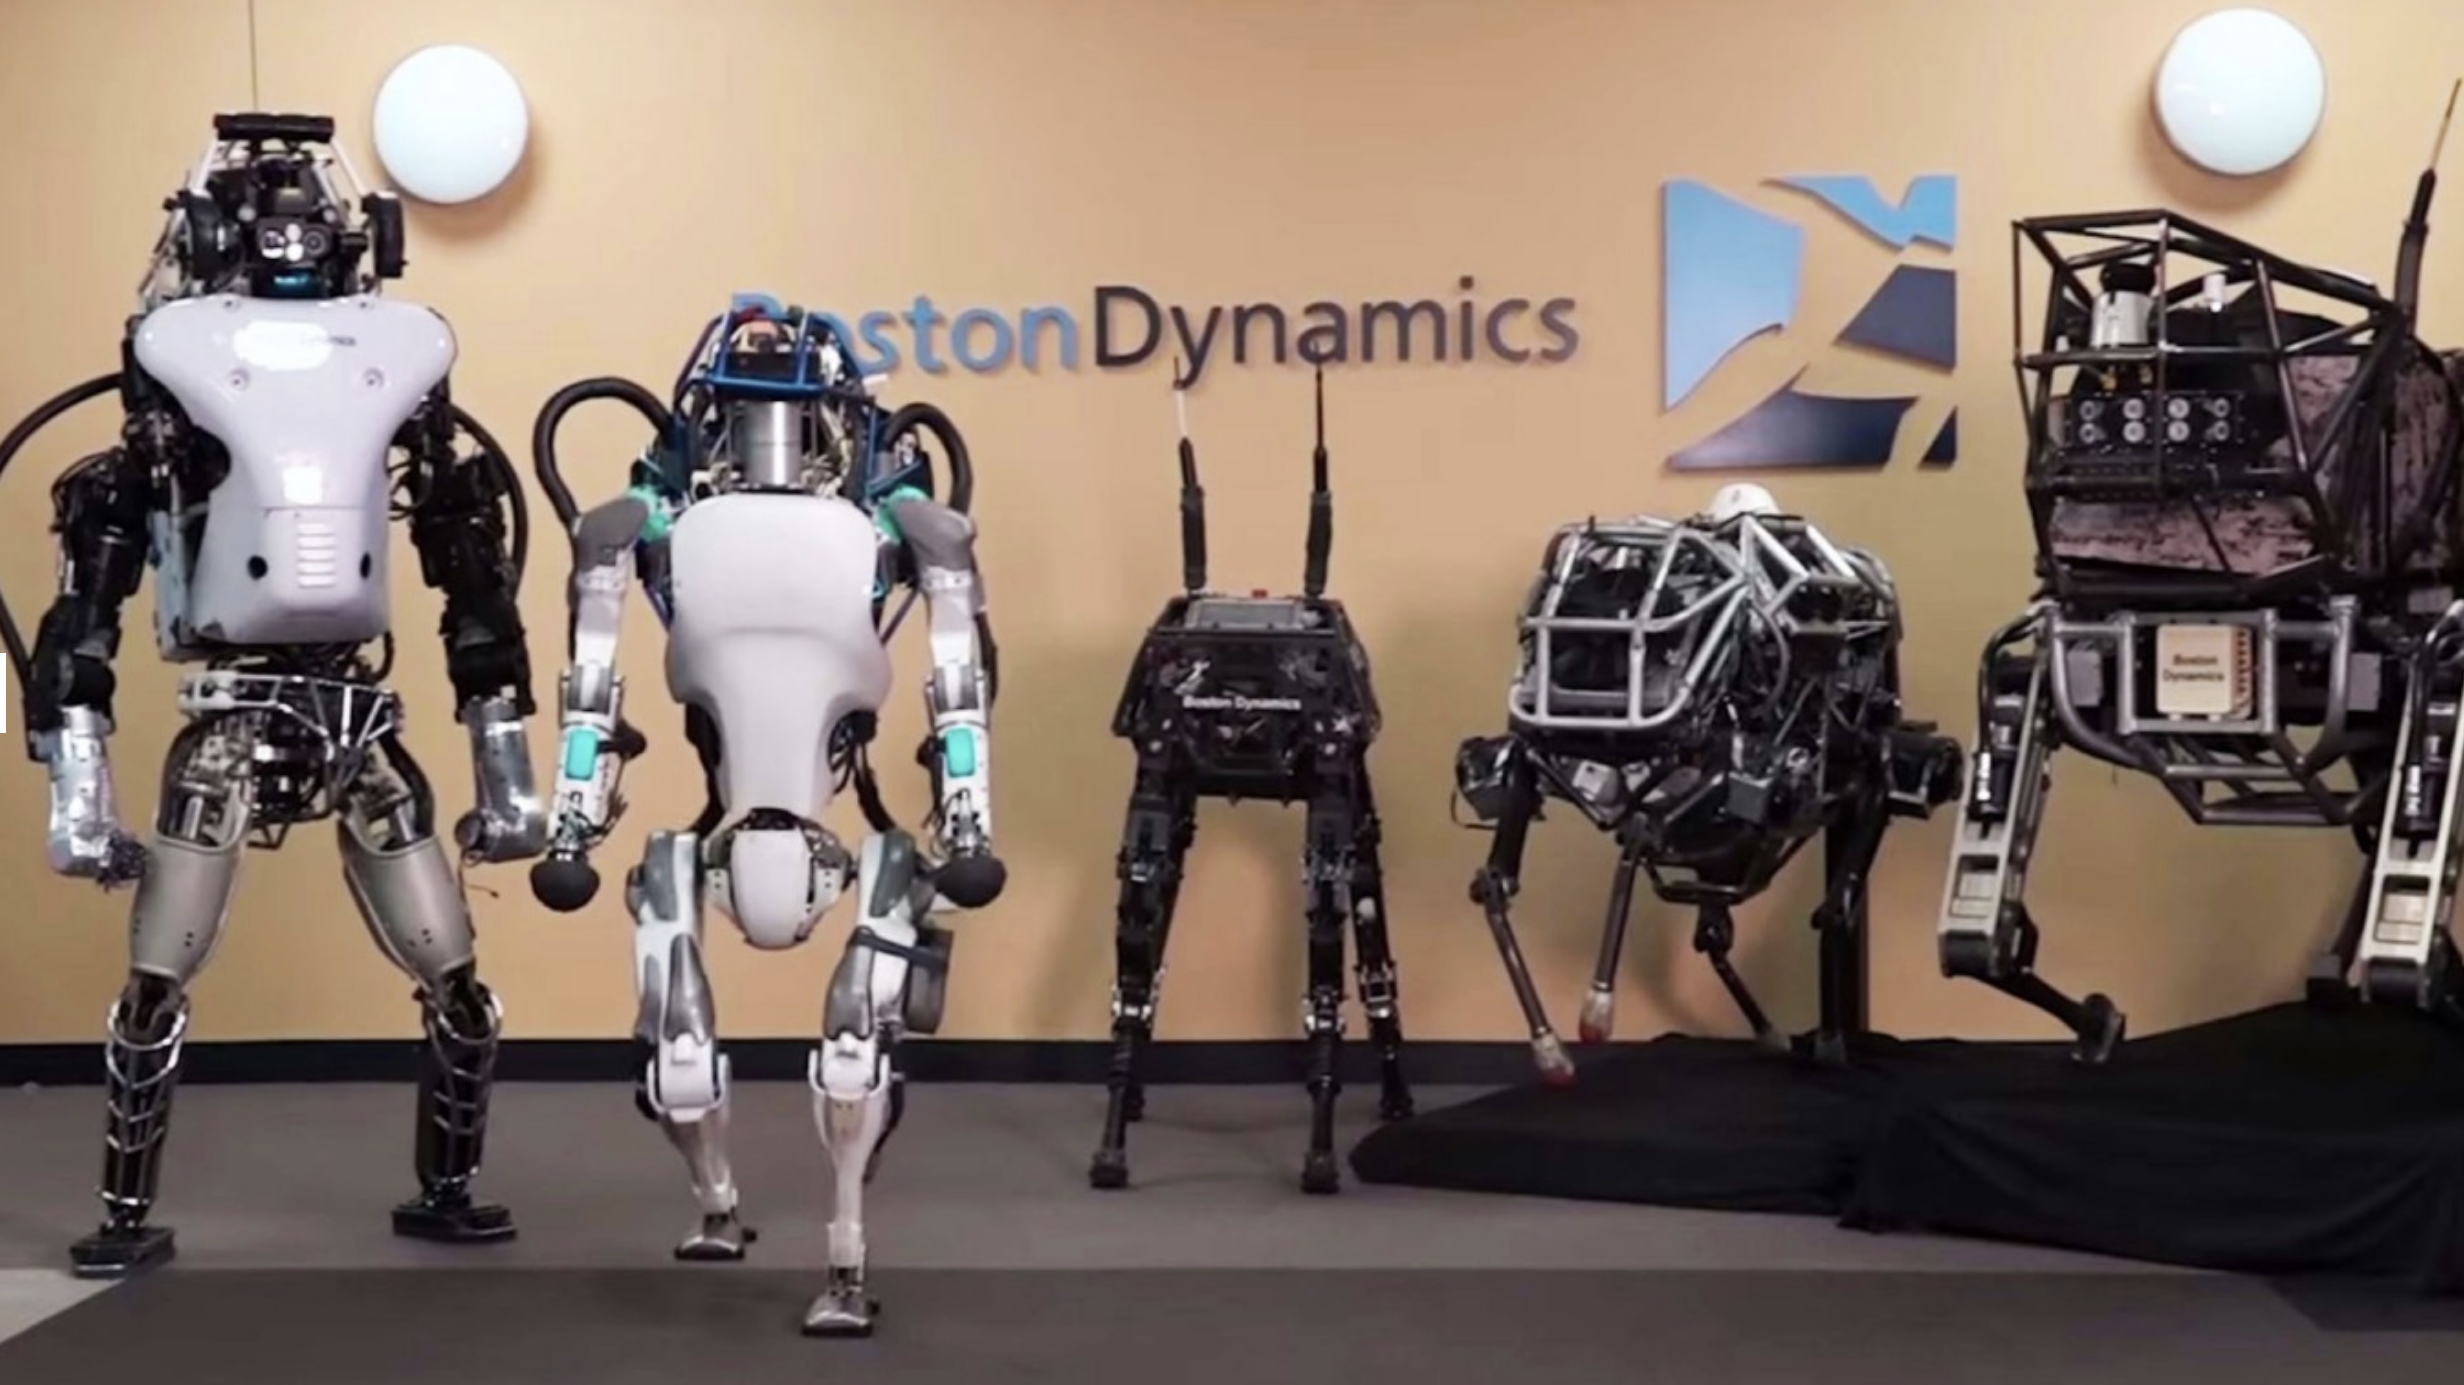
\includegraphics[width=8cm]{figure/bostondynamic.png}
%\caption{Boston Dynamics (\href{https://www.youtube.com/watch?v=fUyU3lKzoio&ab_channel=BostonDynamics}{click here})}
%\end{figure}
%\footnotesize
%\begin{itemize}
%\item Boston Dynamics is a world leader in mobile robots founded in 1992 as a spin-off from the Massachusetts Institute of Technology.
%\vspace{.1cm}
%\item The company is best known for the development of a series of dynamic highly-mobile robots, including BigDog, Spot, Atlas, and Handle.
%\end{itemize}
%\framebreak
%%%%%%%%%%%%%%%%%%%%%%%%%%%%%%%%%%%%%%%%%%%%%%%%%%%%%%%%%%%%%%%%%%

\begin{figure}
\centering
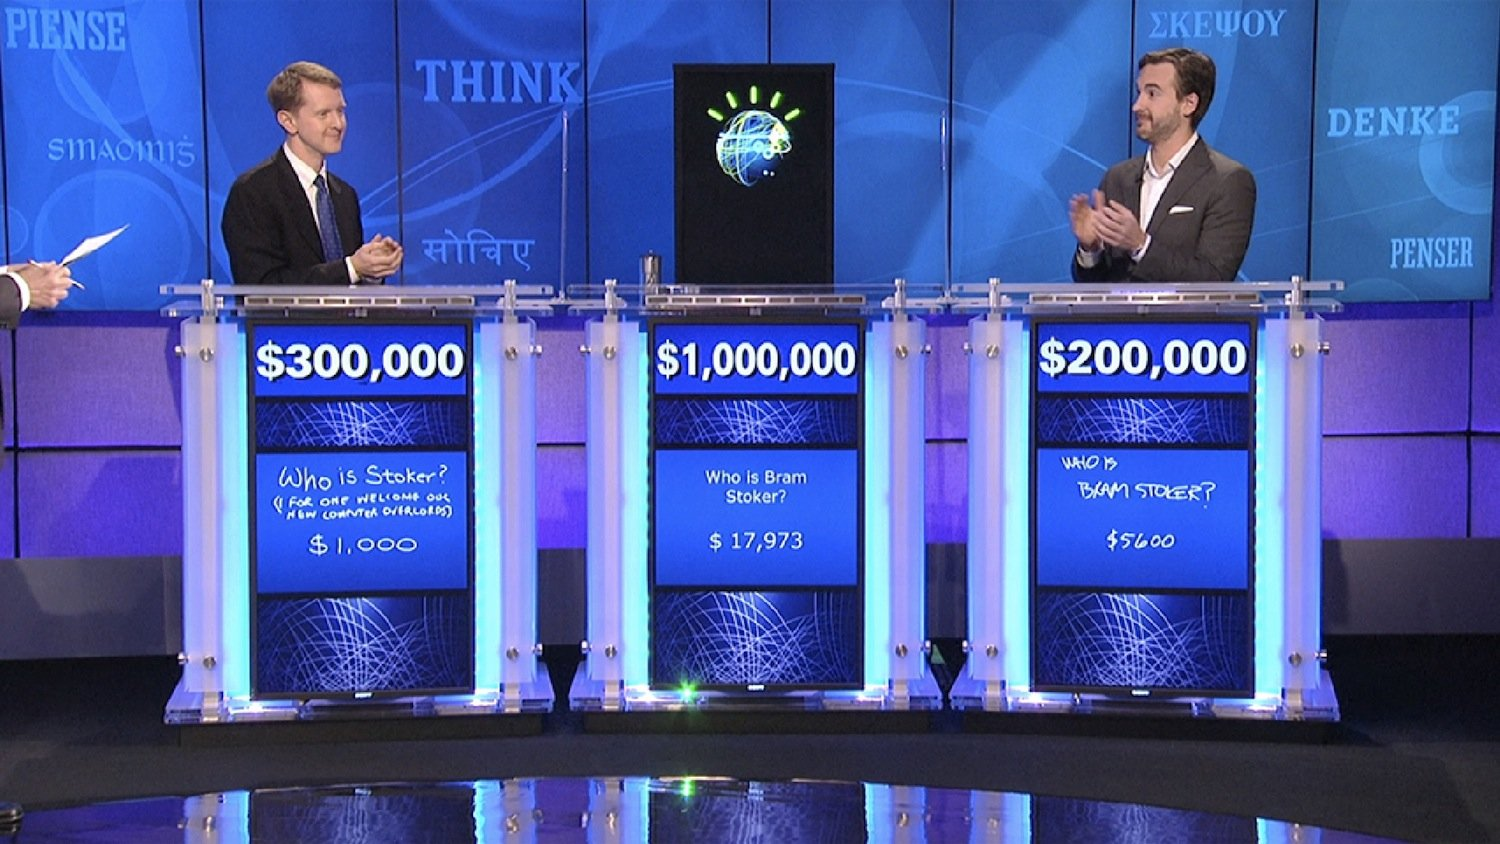
\includegraphics[width=8cm]{figure/ibmsupercomputer.jpg}
\caption{IBM Supercomputer Watson (IBM, 2011)}
\end{figure}
\footnotesize
\begin{itemize}
\item Watson is a question-answering system capable of answering questions posed in natural language, developed in IBM's DeepQA project.
\vspace{.1cm}
\item In 2011, Watson competed on \textit{Jeopardy!} against champions Brad Rutter and Ken Jennings, winning the first place prize of $\$ 1$ million.
\end{itemize}
\framebreak
%%%%%%%%%%%%%%%%%%%%%%%%%%%%%%%%%%%%%%%%%%%%%%%%%%%%%%%%%%%%%%%%%%

\begin{figure}
\centering
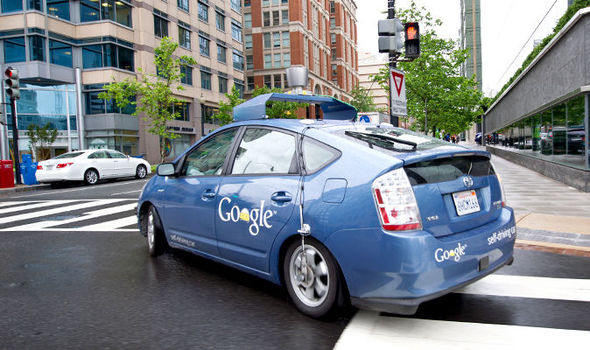
\includegraphics[width=7cm]{figure/selfdriving.jpg}
\caption{Google's self driving car (McCabe, 2016)}
\end{figure}
\footnotesize
\begin{itemize}
\item Google's development of self-driving technology began on January 17, 2009, at the company's secretive X lab.
\vspace{.1cm}
\item By January 2020, $20$ million miles of self-driving on public roads had been completed by Waymo.
\end{itemize}
\framebreak
%%%%%%%%%%%%%%%%%%%%%%%%%%%%%%%%%%%%%%%%%%%%%%%%%%%%%%%%%%%%%%%%%%

\begin{figure}
\centering
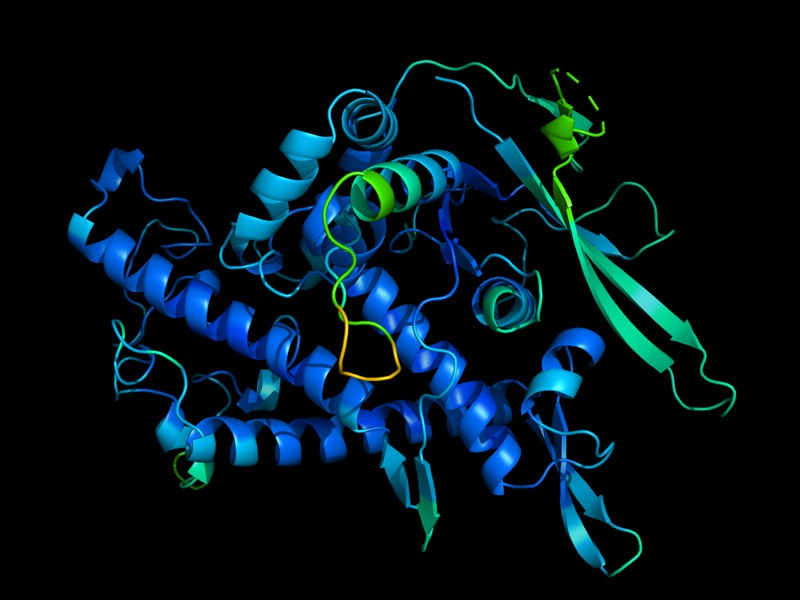
\includegraphics[width=6cm]{figure/alphafold.jpg}
\caption{Protein structure by AlphaFold (DeepMind, 2022)}
\end{figure}
\footnotesize
\begin{itemize}
\item\textbf{AlphaFold} is a deep learning system, developed by Google DeepMind, for determining a protein's 3D shape from its amino-acid sequence.
\vspace{.1cm}
\item In 2018 and 2020, AlphaFold placed first in the overall rankings of the Critical Assessment of Techniques for Protein Structure Prediction (CASP).
\end{itemize}
\framebreak
%%%%%%%%%%%%%%%%%%%%%%%%%%%%%%%%%%%%%%%%%%%%%%%%%%%%%%%%%%%%%%%%%%
\begin{figure}
\centering
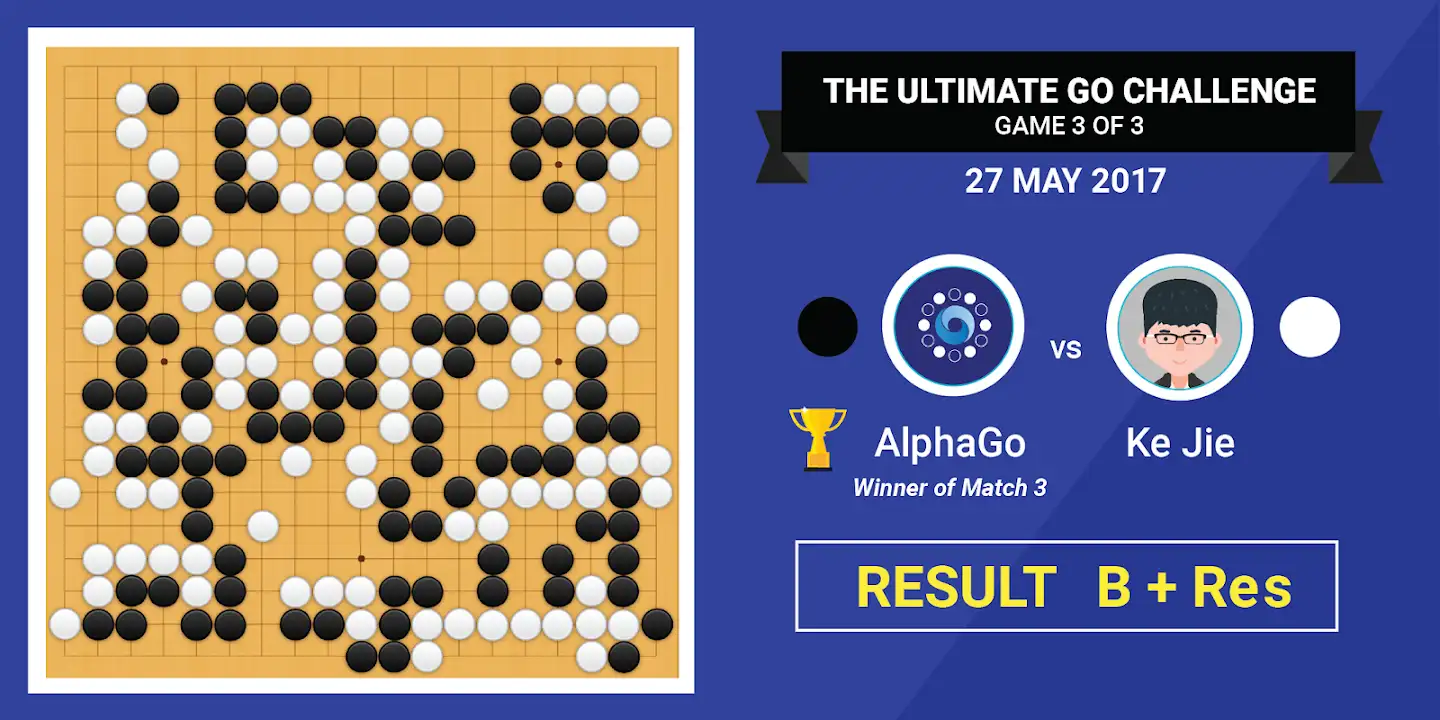
\includegraphics[width=8cm]{figure/alphago.png}
\caption{AlphaGo (DeepMind, 2022)}
\end{figure}
\footnotesize
\begin{itemize}
\item\textbf{AlphaGo}, originally developed by DeepMind, is a deep learning system that plays the board game Go. In 2017, the Master version of AlphaGo beat Ke Jie, the number one ranked player in the world at the time.
\vspace{.1cm}
\item While there are several extensions to AlphaGo (e.g., Master AlphaGo, AlphaGo Zero, AlphaZero, and MuZero), the main idea is the same: search for optimal moves based on knowledge acquired by machine learning.
\end{itemize}
\framebreak
%%%%%%%%%%%%%%%%%%%%%%%%%%%%%%%%%%%%%%%%%%%%%%%%%%%%%%%%%%%%%%%%%%

\begin{figure}
\centering
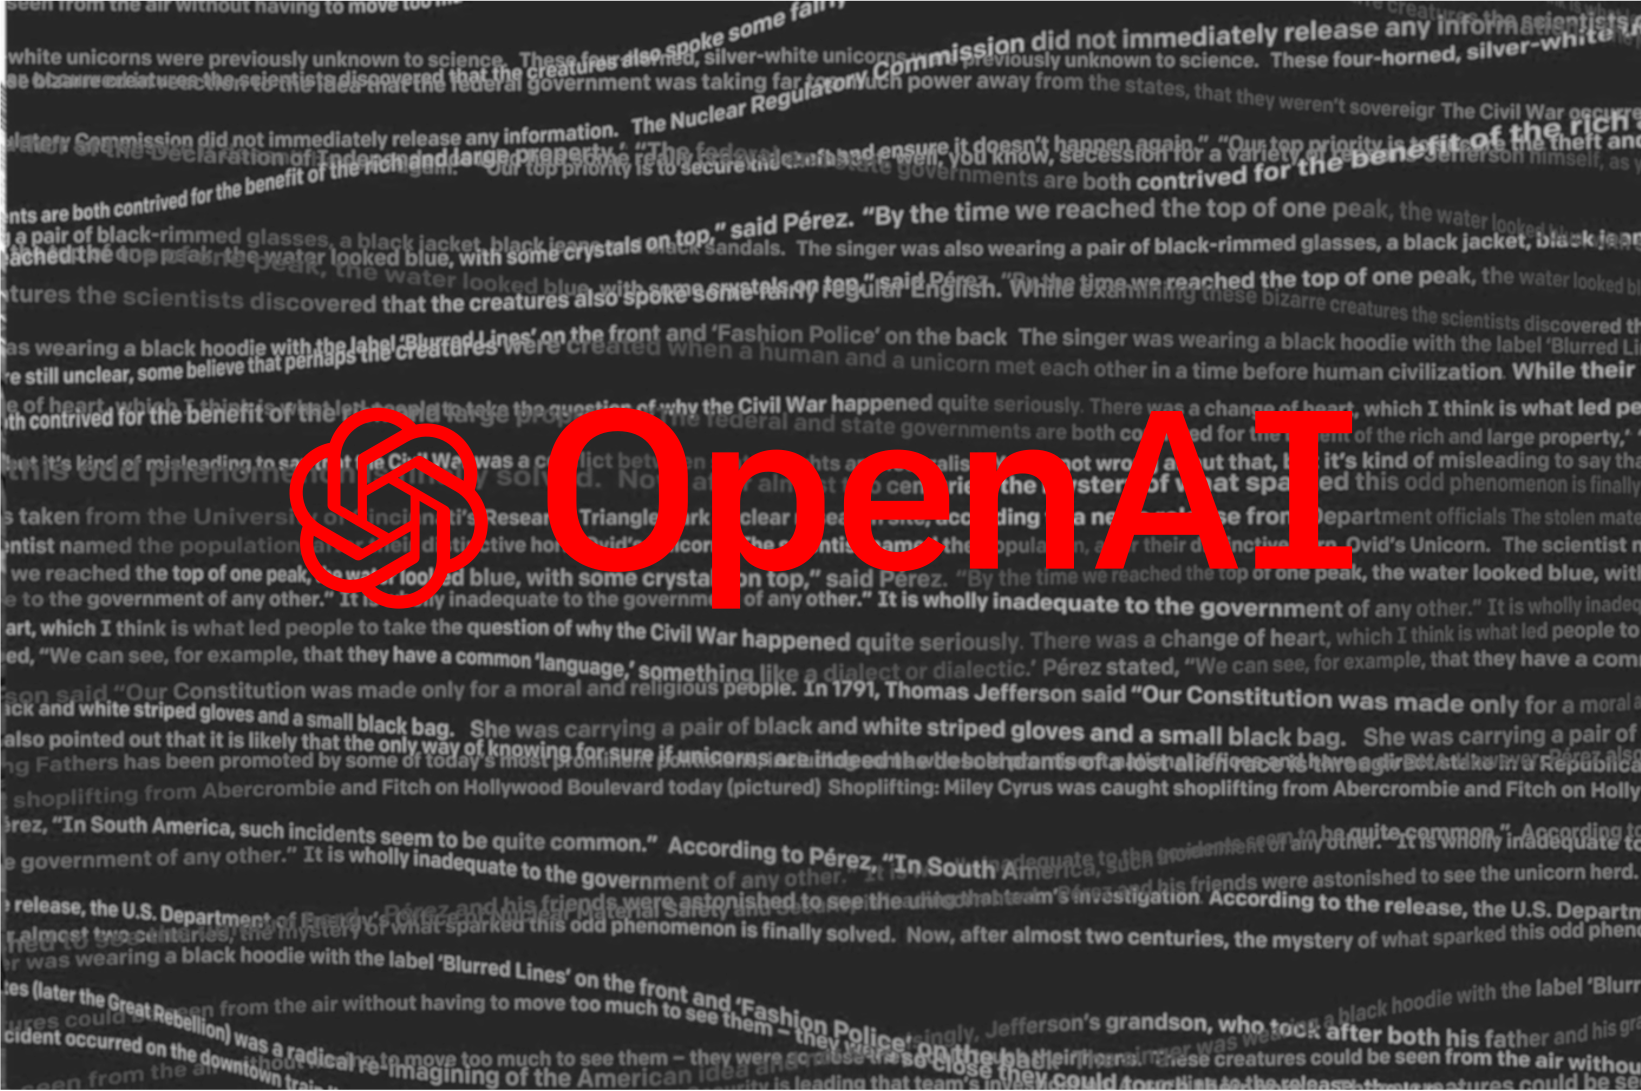
\includegraphics[width=6cm]{figure/gpt3.png}
\caption{Logo OpenAI (OpenAI, 2023)}
\end{figure}
\footnotesize
\begin{itemize}
\item\textbf{Generative Pre-trained Transformer 3 (GPT-3)} is the third generatation of the GPT model, introduced by OpenAI in May 2020, to produce human-like text.
\vspace{.1cm}
\item There are 175 billion parameters to be learned by the algorithm, but the quality of the generated text is so high that it is hardly possible to distinguish it from a human-written text.
\end{itemize}
\end{vbframe}
%%%%%%%%%%%%%%%%%%%%%%%%%%%%%%%%%%%%%%%%%%%%%%%%%%%%%%%%%%%%%%%%%%

\begin{vbframe}{What the field looks like today}
\vspace{.2cm}
\begin{itemize}
  \item A major shift in the 2020s was the move from highly specialized models to \textbf{foundation models}: large pretrained models that can be adapted to many downstream tasks.
\vspace{.1cm}
\item The frontier is increasingly \textbf{multimodal}: models can jointly process text, images, audio, video, and actions.
\vspace{.1cm}
\item Modern systems are also becoming more \textbf{interactive}: they can write code, search, retrieve documents, and call external tools.
\vspace{.1cm}
\item Examples of this broader landscape include \textbf{GPT-5} and \textbf{Claude Opus} for general-purpose assistants, \textbf{Stable Diffusion} for image generation, \textbf{DINOv3} for self-supervised visual representations, and \textbf{TabPFN} for tabular prediction.
\framebreak
\item Progress is now often driven by a combination of
\tiny
\begin{itemize}
\item better architectures and training objectives,
\item much larger datasets,
\item more compute and specialized hardware,
\item stronger software tooling and engineering.
\end{itemize}
\small
The modern DL pipeline is frequently: \textbf{pretrain at scale, then adapt with prompting, finetuning, retrieval, or tool use}.
\end{itemize}
\end{vbframe}


\section{Single Neuron / Perceptron}
%%%%%%%%%%%%%%%%%%%%%%%%%%%%%%%%%%%%%%%%%%%%%%%%%%%%%%%%%%%%%%%%%%

%\begin{frame} {A Single Neuron}
%\begin{itemize}
%\item To illustrate the types of functions that neural networks can represent, let us begin with a simple model: logistic regression.
%\vspace{5mm}
%\item The hypothesis space of logistic regression can be written as follows, where $\tau(z) = (1 + \exp(-z))^{-1}$ is the logistic sigmoid function:
%\begin{small} 
%$$\Hspace = \left\{f: \R^p \to [0, 1] ~\bigg|~ \fx = \tau\left(\sum_{j = 1}^p w_j x_j + b\right), \wtw \in \R^p, b \in \R \right\},$$ \end{small}
%\vspace{3mm}
%\item It is straightforward to represent $\fx$ graphically as a neuron.
%\vspace{5mm}
%\item Note: $\wtw$ and $b$ together constitute $\thetab$.
%\end{itemize}
%\end{frame}
%%%%%%%%%%%%%%%%%%%%%%%%%%%%%%%%%%%%%%%%%%%%%%%%%%%%%%%%%%%%%%%%%%

\begin{vbframe} {A Single Neuron}
\vspace{-0.6cm}
\begin{figure}
\centering
\scalebox{1}{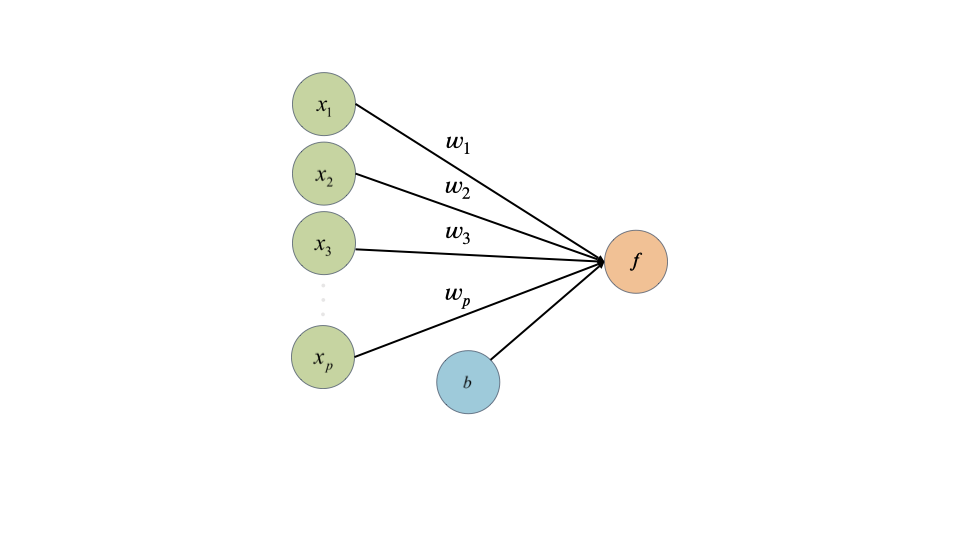
\includegraphics{figure/perceptron_tau.png}}
\end{figure}
\vspace{-1.8cm}
\footnotesize Perceptron %$z$, 
with \textbf{input features} $x_1, x_2, ... ,x_p$, \textbf{weights} $w_1, w_2,... ,w_p$, \textbf{bias term} $b$, and \textbf{activation function} $\tau$.
\vspace{.2cm}
\normalsize
\begin{itemize}
\item The perceptron is a single artificial neuron and the basic computational unit of neural networks.
\vspace{.2cm}
\item It is a weighted sum of input values, transformed by $\tau$:
\vspace{-1mm}
$$f(\mathbf{x}) = \tau(w_1x_1 + ... + w_px_p +  b) = \tau(\mathbf{w}^T \mathbf{x}+b)$$
\end{itemize}
\end{vbframe}
%%%%%%%%%%%%%%%%%%%%%%%%%%%%%%%%%%%%%%%%%%%%%%%%%%%%%%%%%%%%%%%%%%

\begin{vbframe}{A Single Neuron}
\textbf{Activation function $\tau$:} a single neuron %can
 represents different functions %i%f we choose a suitable activation function for it.
 depending on the choice of activation function.
\vspace{.5cm}
\begin{itemize}
\item The identity function gives us the simple \textbf{linear regression}:
$$f(\mathbf{x}) = \tau(\mathbf{w}^T \mathbf{x}) = \mathbf{w}^T \mathbf{x}$$
%\vspace{.5cm}
\item The logistic function gives us the \textbf{logistic regression}:
$$f(\mathbf{x}) = \tau(\mathbf{w}^T \mathbf{x}) = \frac{1}{1 + \exp(-\mathbf{w}^T \mathbf{x})}$$
\end{itemize}
\end{vbframe}
%%%%%%%%%%%%%%%%%%%%%%%%%%%%%%%%%%%%%%%%%%%%%%%%%%%%%%%%%%%%%%%%%%

\begin{vbframe} {A Single Neuron}
We consider a %logistic regression model for
 perceptron with
$3$-dimensional input, i.e. $\fx = \tau(w_1\textcolor{red}{x_1} + w_2\textcolor{red}{x_2} + w_3\textcolor{red}{x_3} + b)$.
\begin{itemize}
\item %First, 
Input features $\xv$ are represented by nodes in the \enquote{input layer}.
\begin{figure}
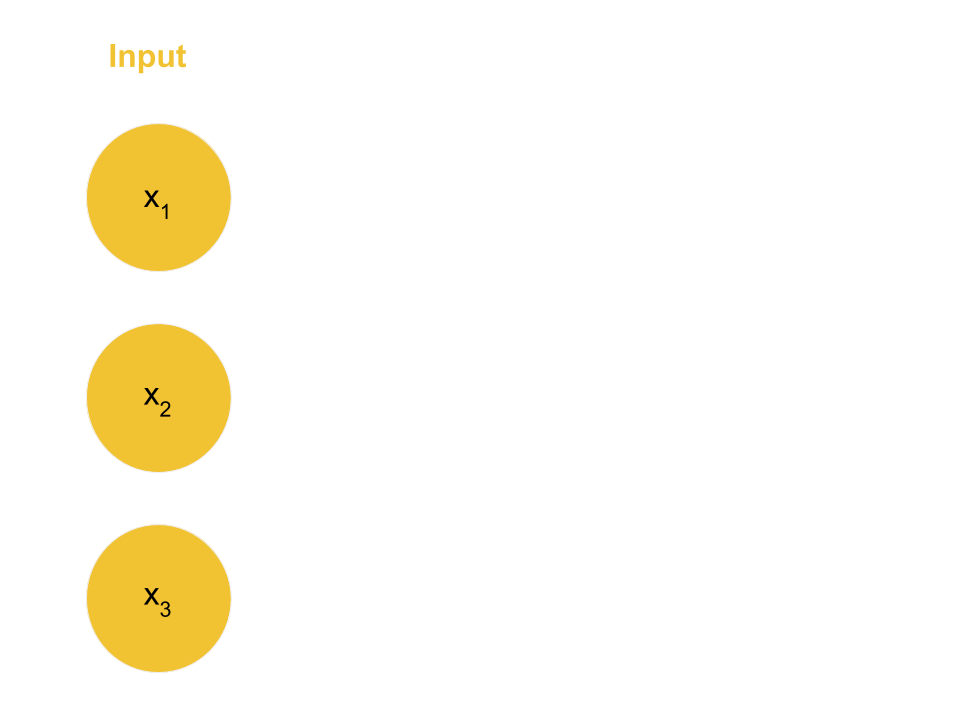
\includegraphics[width=6cm]{figure/neurep_one.png}
\end{figure}
\item In general, a $p$-dimensional input vector $\xv$ will be represented by $p$ nodes in the input layer.
\framebreak
%%%%%%%%%%%%%%%%%%%%%%%%%%%%%%%%%%%%%%%%%%%%%%%%%%%%%%%%%%%%%%%%%%

\item %Next, 
Weights $\mathbf{w}$ are connected to edges from the input layer.
\begin{figure}
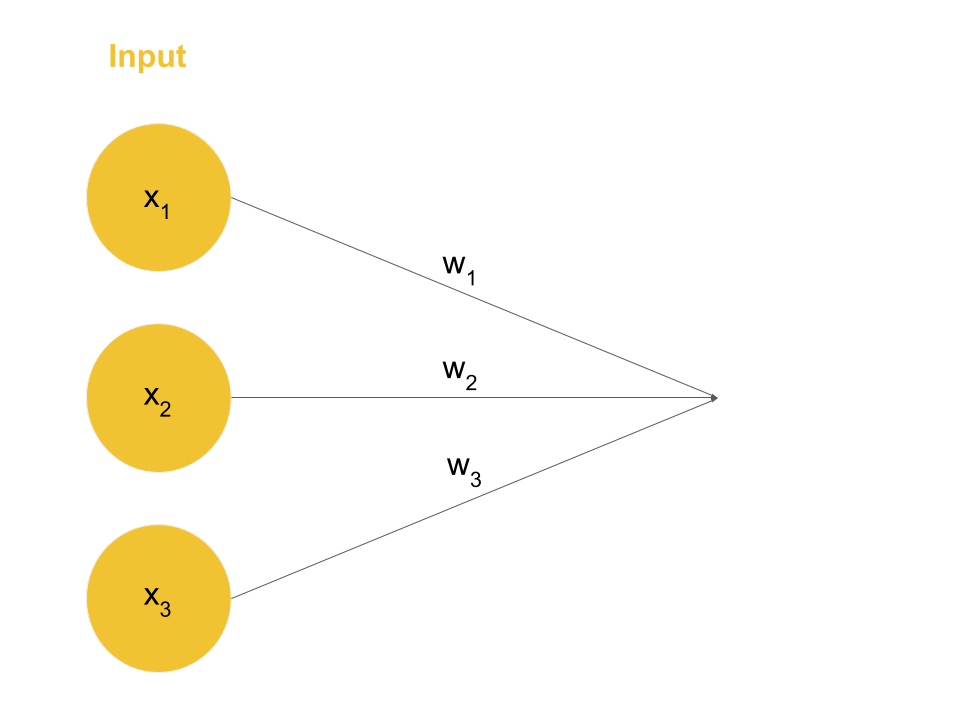
\includegraphics[width=6cm]{figure/neurep_two.png}
\end{figure}
\item The bias term $b$ is implicit here. It is often not visualized as a separate node.
\end{itemize}
\framebreak
%%%%%%%%%%%%%%%%%%%%%%%%%%%%%%%%%%%%%%%%%%%%%%%%%%%%%%%%%%%%%%%%%%

For an explicit graphical representation, we do a simple trick: 
\begin{itemize}
\item Add a constant feature to the inputs $\tilde{\xv} = (1, x_1, ..., x_p)^T$
\item and absorb the bias into the weight vector $\tilde{\bm{w}} = (b, w_1, ..., w_p)$.
\end{itemize}
The graphical representation is then: 
\begin{figure}
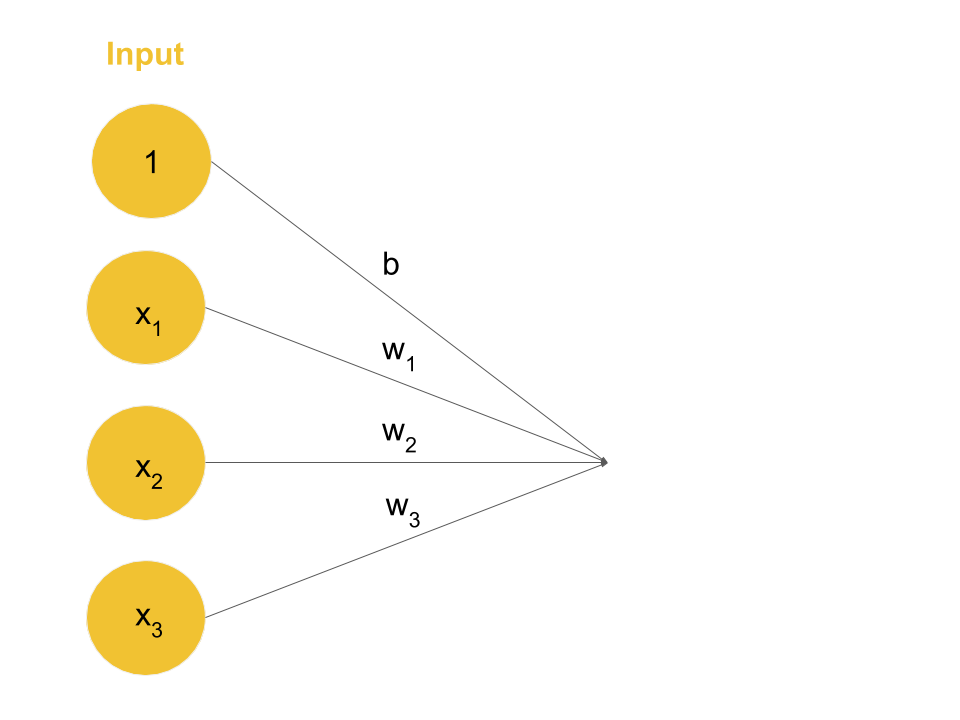
\includegraphics[width=7cm]{figure/neurep_bias.png}
\end{figure}
\framebreak
%%%%%%%%%%%%%%%%%%%%%%%%%%%%%%%%%%%%%%%%%%%%%%%%%%%%%%%%%%%%%%%%%%

\begin{itemize}
\item %Finally, 
The computation $\tau(w_1x_1 + w_2x_2 + w_3x_3 + b)$ is represented by the neuron in the \enquote{output layer}.
\begin{figure}
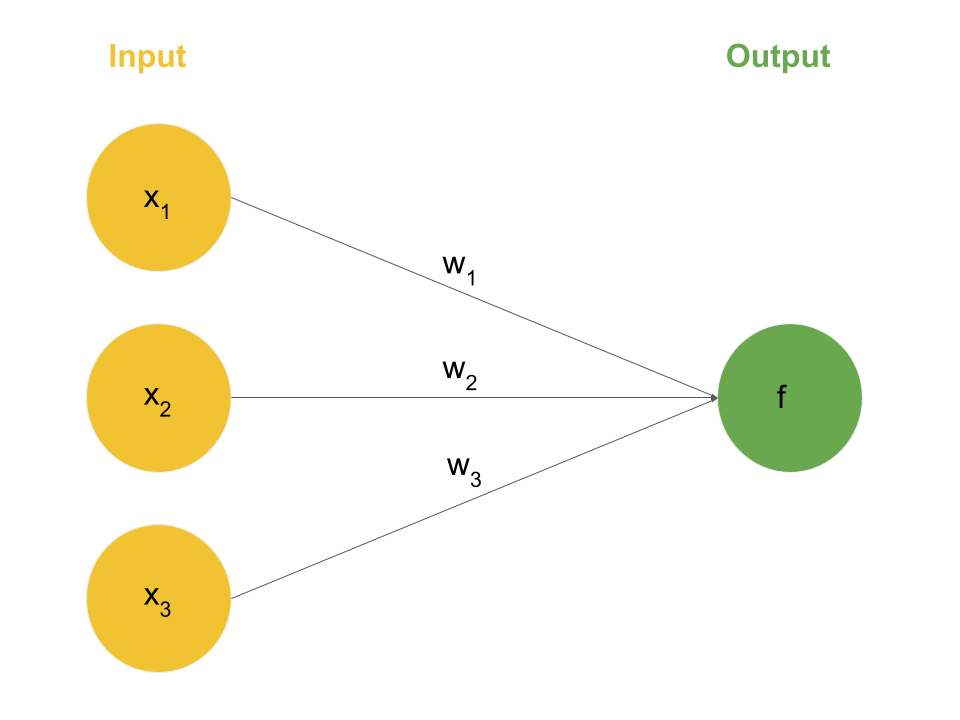
\includegraphics[width=6cm]{figure/neurep_three.png}
\end{figure}
%\item Because this single neuron represents exactly the same hypothesis space as logistic regression, it can only learn linear decision boundaries.
\framebreak
%%%%%%%%%%%%%%%%%%%%%%%%%%%%%%%%%%%%%%%%%%%%%%%%%%%%%%%%%%%%%%%%%%

\item %A nice thing about this graphical representation of functions is that 
You can picture the input vector being "fed" to neurons on the left followed by a sequence of computations performed from left to right. This is called a \textbf{forward pass}.
\end{itemize}
\vspace{1cm}
\begin{figure}
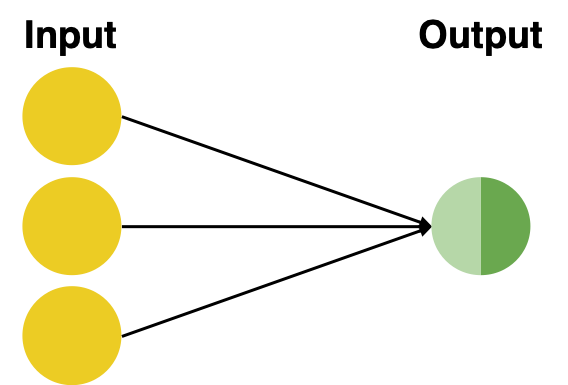
\includegraphics[width=5.5cm]{figure/forward_pass.png}
\end{figure}
\end{vbframe}
%%%%%%%%%%%%%%%%%%%%%%%%%%%%%%%%%%%%%%%%%%%%%%%%%%%%%%%%%%%%%%%%%%

\begin{frame} {A Single Neuron}
A neuron performs a 2-step computation:
\begin{enumerate}
\item \textbf{Affine Transformation:} weighted sum of inputs plus bias.
\begin{figure}
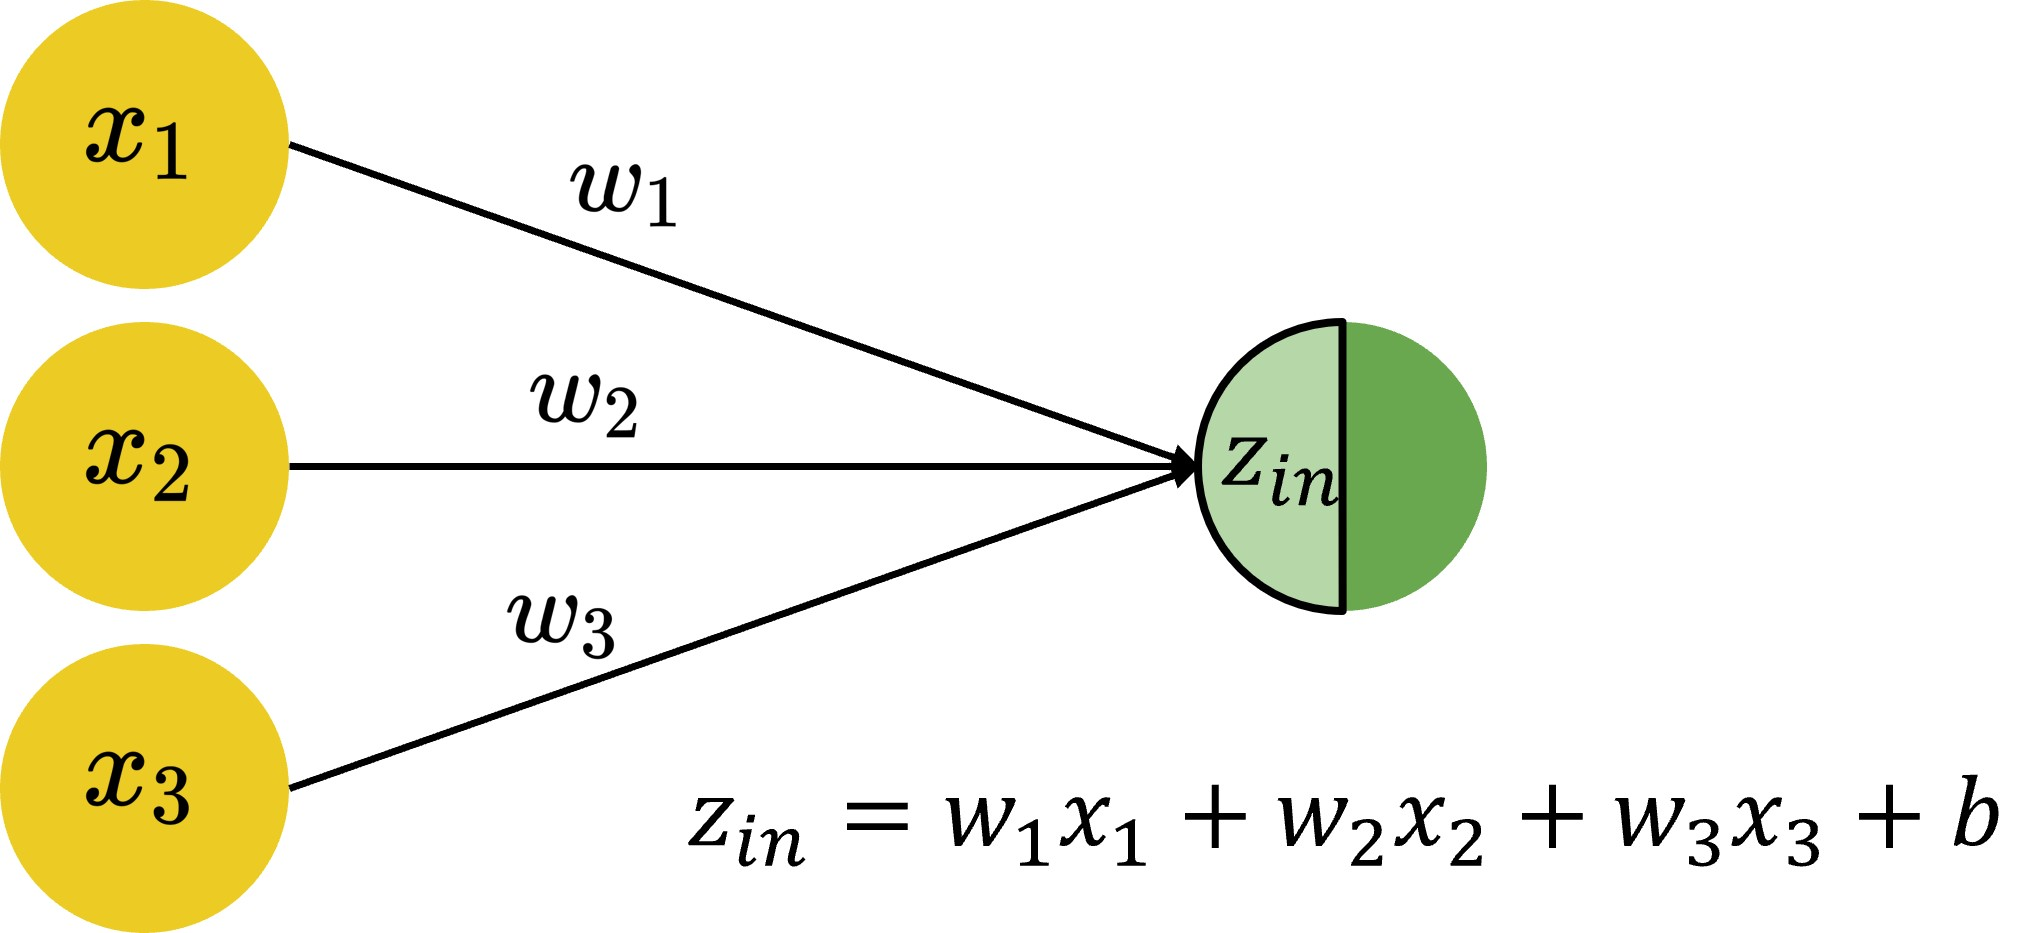
\includegraphics[width=5.5cm]{figure/step1-zin.jpg}
\end{figure}
\item \textbf{Non-linear Activation:} a non-linear transformation applied to the weighted sum.
\begin{figure}
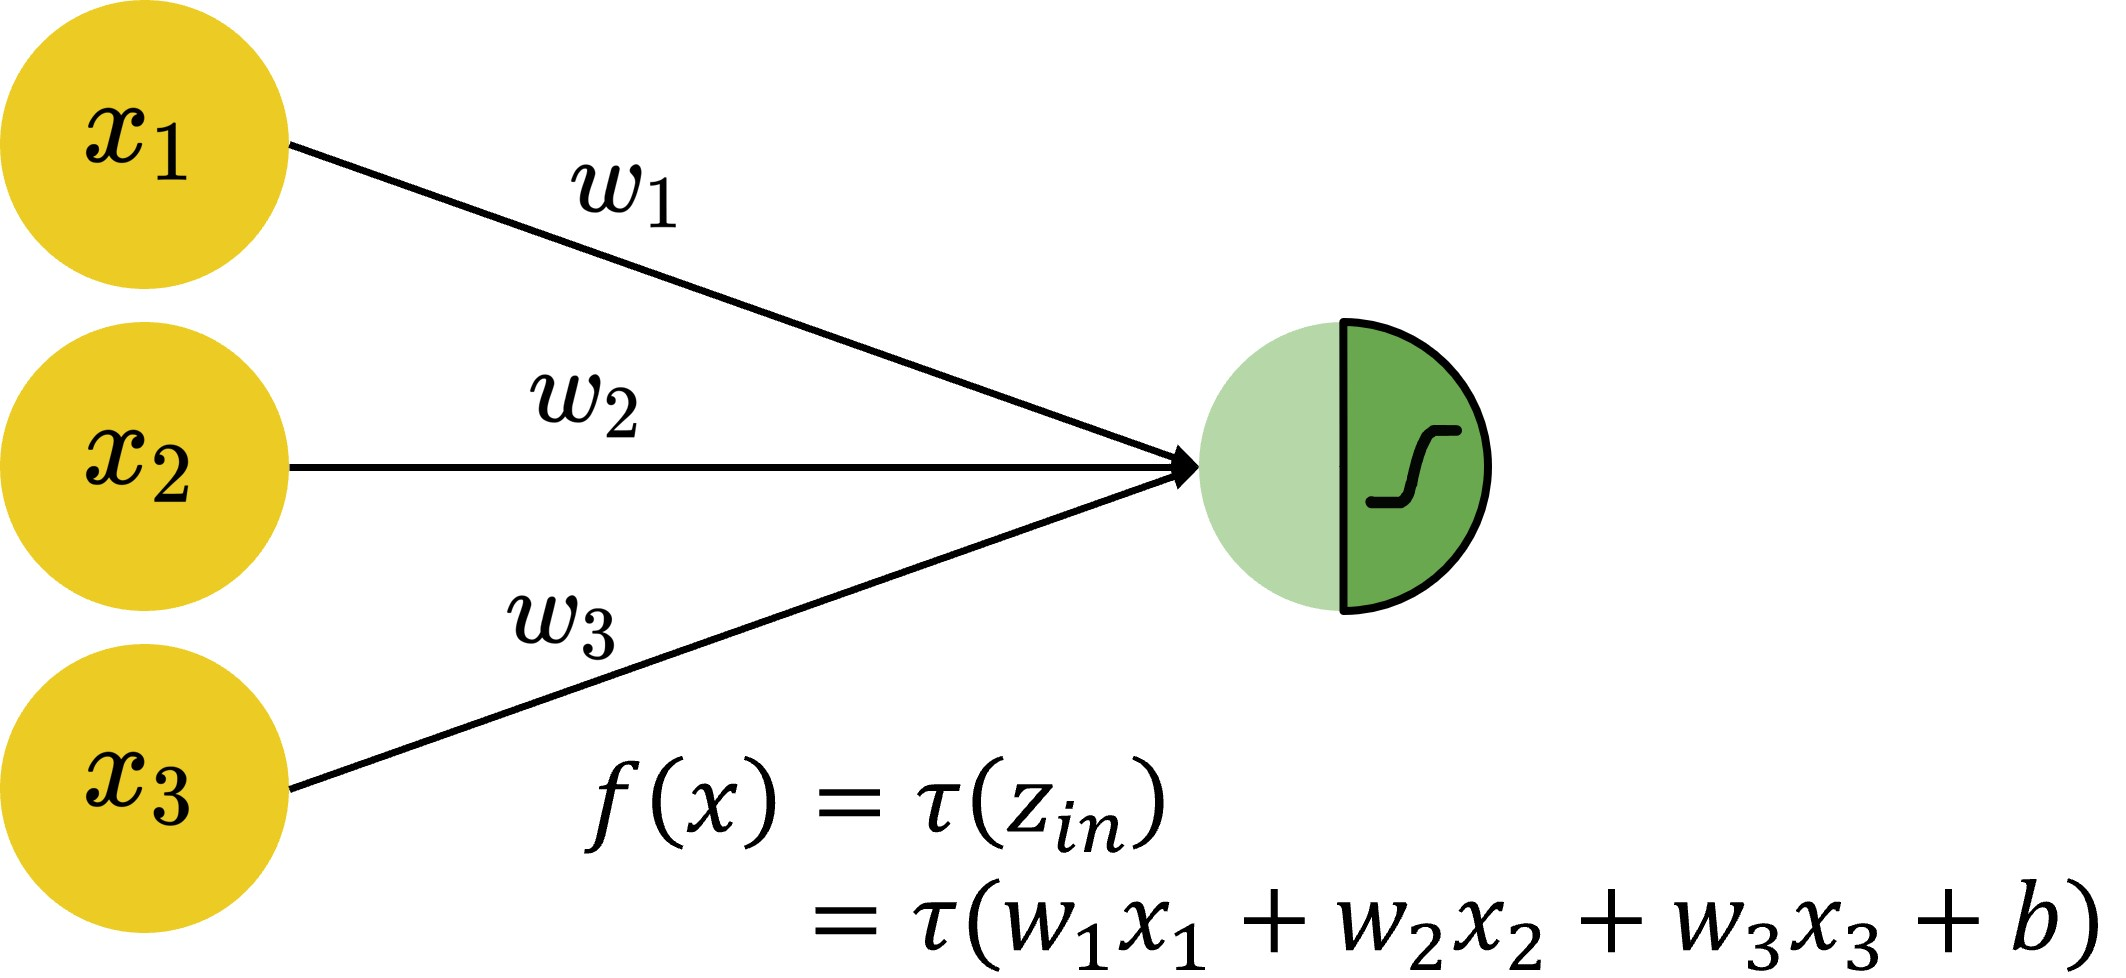
\includegraphics[width=5.5cm]{figure/step2-zin.jpg}
\end{figure}
\end{enumerate}
\end{frame}
%%%%%%%%%%%%%%%%%%%%%%%%%%%%%%%%%%%%%%%%%%%%%%%%%%%%%%%%%%%%%%%%%%

%\begin{vbframe} {A Single Neuron}
%\begin{itemize}
%\item Even though all neurons compute a weighted sum in the first step, there is considerable flexibility in the type of activation function used in the second step.
%\item For example, setting the activation function to the logistic sigmoid function allows a neuron to represent logistic regression. The following architecture with two neurons represents two logistic regressions using the same input features:
%\end{itemize}
%\begin{figure}
%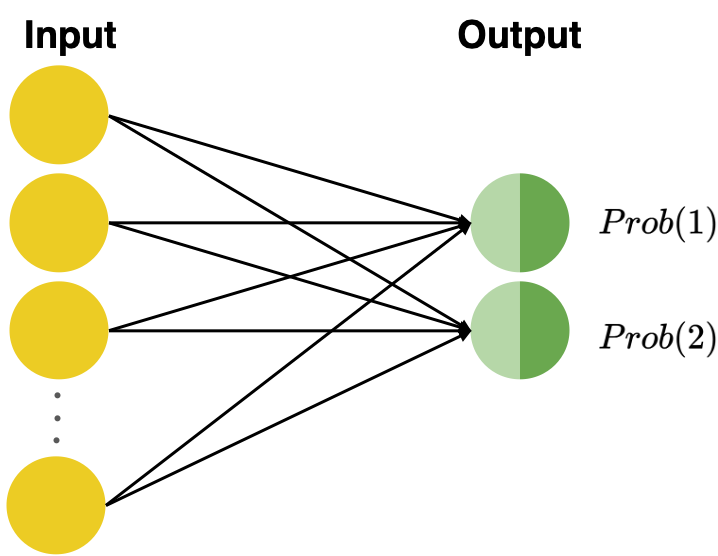
\includegraphics[width=5cm]{figure/logistic_regression.png}
%\end{figure}
%\end{vbframe}
%%%%%%%%%%%%%%%%%%%%%%%%%%%%%%%%%%%%%%%%%%%%%%%%%%%%%%%%%%%%%%%%%%%

\begin{vbframe}{A Single Neuron: Hypothesis Space}
\begin{itemize}
\item The hypothesis space that is formed by single neuron %architectures 
is 
\begin{small}
$$\Hspace  = \left\{f: \R^p \to \R ~\bigg|~ \fx = \tau\left(\sum_{j = 1}^p w_j x_j + b\right), \wtw \in \R^p, b \in \R\right\}.$$ 
\end{small}
%\item Both logistic regression and linear regression are subspaces of $\Hspace$ (if $\tau$ is the logistic sigmoid / identity function).  
\item If $\tau$ is the logistic sigmoid or identity function, $\Hspace$ corresponds to the hpothesis space of logistic or linear regression, respectively.
\end{itemize}
\vspace*{-0.45cm}
\begin{figure}
\centering
\scalebox{0.6}{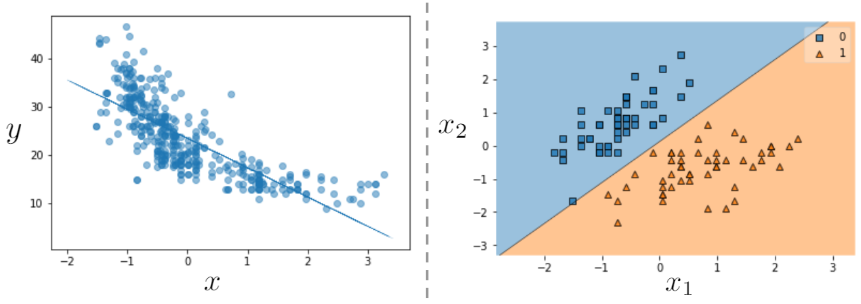
\includegraphics{figure/neuron_regcls.png}}
\vspace*{-0.2cm}
\begin{tiny}
\caption{\textit{Left}: A regression line learned by a single neuron. \textit{Right}: A decision-boundary learned by a single neuron in a binary classification task.}
\end{tiny}
\end{figure}
\end{vbframe}
%%%%%%%%%%%%%%%%%%%%%%%%%%%%%%%%%%%%%%%%%%%%%%%%%%%%%%%%%%%%%%%%%%

\begin{vbframe} {A Single Neuron: Optimization}
\begin{itemize}
\item To optimize this model, we minimize the empirical risk 
$$\riske = \frac{1}{n} \sumin \Lxyi,$$
where $\Lxy$ is a loss function. It compares the network's predictions $\fx$ to the ground truth $y$. 
\item For regression, we typically use the L2 loss (rarely L1): $$\Lxy = \frac{1}{2}(y - \fx)^2$$
\item For binary classification, we typically apply the cross entropy loss (also known as Bernoulli loss): $$\Lxy = -(y \log \fx + (1 - y) \log(1 - \fx))$$
\framebreak 
%%%%%%%%%%%%%%%%%%%%%%%%%%%%%%%%%%%%%%%%%%%%%%%%%%%%%%%%%%%%%%%%%%

\vspace{.5cm}
\item For a single neuron and both choices of $\tau$ the loss function is convex.
\item The global optimum can be found with an iterative algorithm like gradient descent. 
\item A single neuron with logistic sigmoid function trained with the Bernoulli loss %does not only have 
%has the same hypothesis space as a logistic regression %and is therefore the same model, but
 %will also 
 yields the %very 
 same result as logistic regression when trained until convergence.
\item Note: In the case of regression and the L2-loss, the solution can
also be found analytically using the “normal equations”. However, in other cases a closed-form solution is usually not available.
\end{itemize}
\end{vbframe} 
%%%%%%%%%%%%%%%%%%%%%%%%%%%%%%%%%%%%%%%%%%%%%%%%%%%%%%%%%%%%%%%%%%


\section{Single Hidden Layer Neural Networks}
%%%%%%%%%%%%%%%%%%%%%%%%%%%%%%%%%%%%%%%%%%%%%%%%%%%%%%%%%%%%%%%%%%

\begin{vbframe}{Motivation}
\lz
\begin{itemize}
\item The graphical way of representing simple functions/models, like logistic regression. Why is that useful?
\lz
\item Because individual neurons can be used as building blocks of more complicated functions.
\lz
\item Networks of neurons can represent extremely complex hypothesis spaces.
\lz
\item Most importantly, it allows us to define the \enquote{right} kinds of hypothesis spaces to learn functions that are %more 
common in our universe in a data-efficient way (see Lin, Tegmark et al. 2016).
\end{itemize}
\framebreak
%%%%%%%%%%%%%%%%%%%%%%%%%%%%%%%%%%%%%%%%%%%%%%%%%%%%%%%%%%%%%%%%%%
Can a single neuron perform binary classification of these points?
%\vspace{2cm}
\begin{figure}
\centering
\scalebox{0.5}{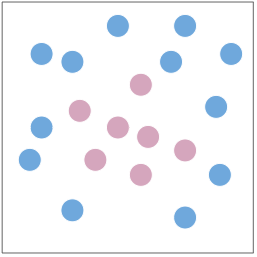
\includegraphics{figure/cartesian.png}}
\end{figure}

\framebreak

\begin{itemize}
\item As a single neuron is restricted to learning only linear decision boundaries, its performance on the following task is quite poor:
\begin{figure}
\centering
\scalebox{0.24}{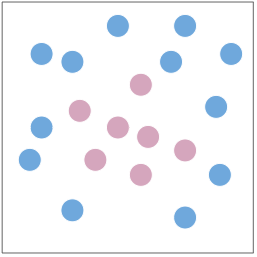
\includegraphics{figure/cartesian.png}}
\end{figure}
\item However, the neuron can easily separate the classes if the original features are transformed (e.g., from Cartesian to polar coordinates): 
\begin{figure}
\centering
\scalebox{0.24}{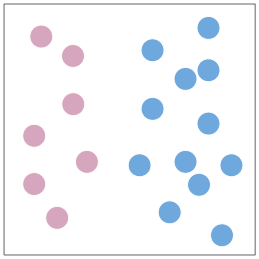
\includegraphics{figure/polar.png}}
\end{figure}
\end{itemize}
\framebreak
%%%%%%%%%%%%%%%%%%%%%%%%%%%%%%%%%%%%%%%%%%%%%%%%%%%%%%%%%%%%%%%%%%

\begin{itemize}
\item Instead of classifying the data in the original representation,
\begin{figure}
\centering
\scalebox{1}{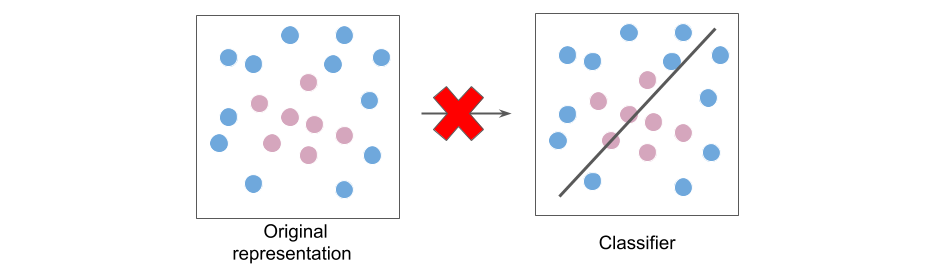
\includegraphics{figure/repold_f.png}}
\end{figure}
\item we classify it in a new feature space.
\begin{figure}
\centering
\scalebox{1}{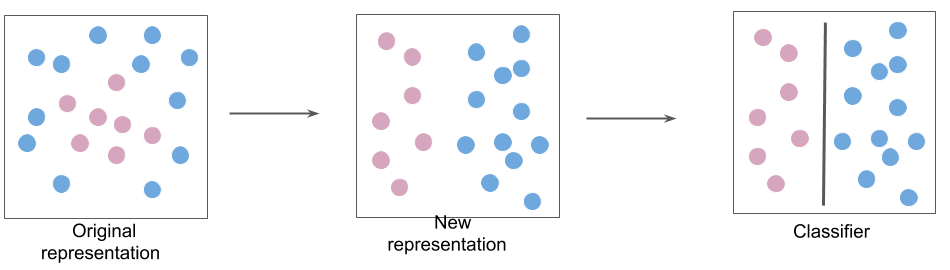
\includegraphics{figure/repnew_f.png}}
\end{figure}
\end{itemize}
\framebreak
%%%%%%%%%%%%%%%%%%%%%%%%%%%%%%%%%%%%%%%%%%%%%%%%%%%%%%%%%%%%%%%%%%

\begin{itemize}
\item Analogously, instead of a single neuron, 
\begin{figure}
\centering
\scalebox{0.6}{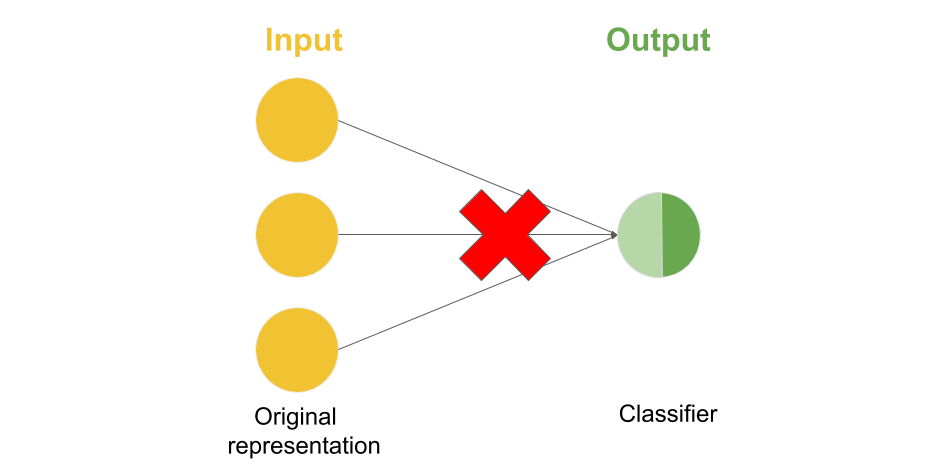
\includegraphics{figure/oldrep_n_f.png}}
\end{figure}
\item we use more complex networks.
\begin{figure}
\centering
\scalebox{0.6}{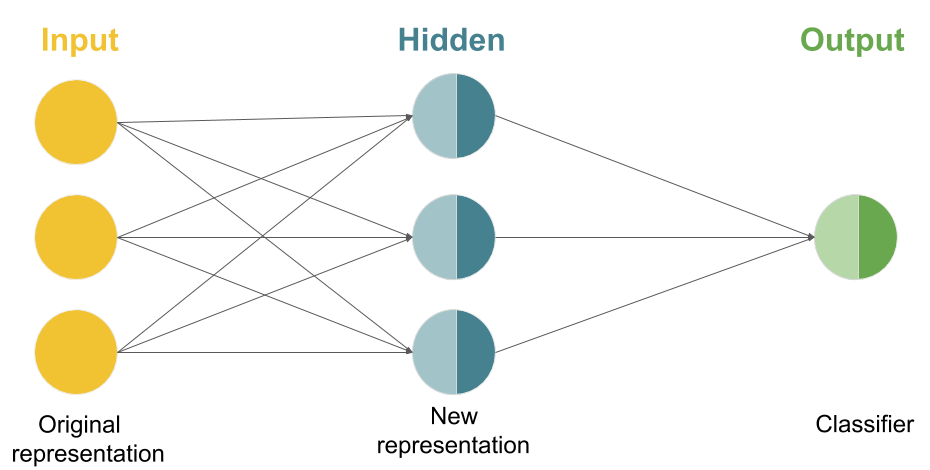
\includegraphics{figure/newrep_n_f.png}}
\end{figure}
\end{itemize}
\end{vbframe}
%%%%%%%%%%%%%%%%%%%%%%%%%%%%%%%%%%%%%%%%%%%%%%%%%%%%%%%%%%%%%%%%%%

\begin{vbframe} {Representation Learning}
  \begin{itemize}
    \vspace{5mm}
    \item It is %therefore 
    \textit{very} critical to feed a classifier the \enquote{right} features in order for it to perform well.
    \vspace{7mm}
    \item Before deep learning took off, features for tasks like machine vision and speech recognition were \enquote{hand-designed} by domain experts. This step of the machine learning pipeline is called \textbf{feature engineering}.
    \vspace{7mm}
    \item %The single biggest reason
     DL %is so important is that it 
    automates feature engineering. This is called \textbf{representation learning}.
  \end{itemize}
\end{vbframe}
%%%%%%%%%%%%%%%%%%%%%%%%%%%%%%%%%%%%%%%%%%%%%%%%%%%%%%%%%%%%%%%%%%

\begin{vbframe}{Single Hidden Layer Networks}
\textbf{Single neurons} perform a 2-step computation:
\begin{enumerate}
\item \textbf{Affine Transformation:} a weighted sum of inputs plus bias.
\item \textbf{Activation:} a non-linear transformation on the weighted sum.
\end{enumerate}
\vspace{.5cm}
\textbf{Single hidden layer networks} consist of two layers (without input layer):
\begin{enumerate}
\item \textbf{Hidden Layer:} having a set of neurons.
\item \textbf{Output Layer:} having one or more output neurons.
\end{enumerate}
\vspace{.5cm}
\begin{itemize}
\item Multiple inputs are simultaneously fed to the network.
\vspace{.2cm}
\item Each neuron in the hidden layer performs a 2-step computation.
\vspace{.2cm}
\item The final output of the network is then calculated by another 2-step computation performed by the neuron in the output layer.
\end{itemize}
\end{vbframe}
%%%%%%%%%%%%%%%%%%%%%%%%%%%%%%%%%%%%%%%%%%%%%%%%%%%%%%%%%%%%%%%%%%  5

\begin{frame} {Single Hidden Layer Networks: Example}
Each neuron in the hidden layer performs an \textbf{affine transformation} on the inputs:
\begin{figure}
\centering
\only<1>{\scalebox{.62}{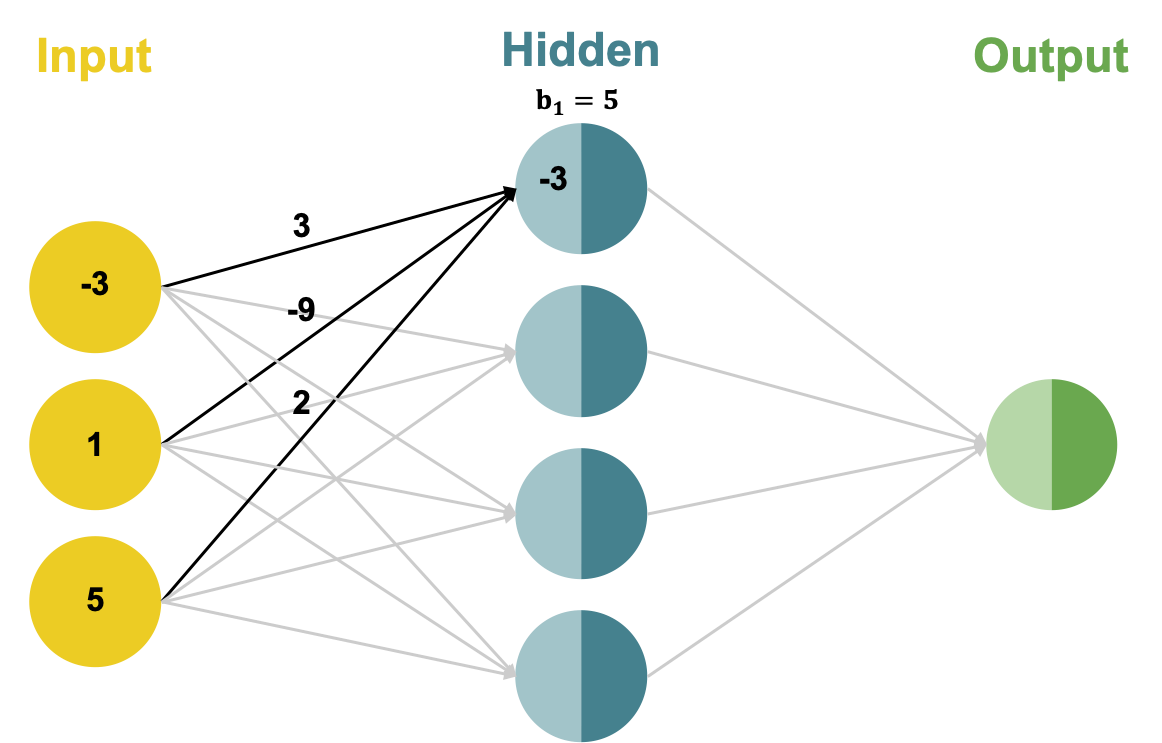
\includegraphics{figure/singlelay_1.png}} $$\begin{array}{l}
z_{\text {1,in}}=w_{11} x_1+w_{21} x_2+w_{31} x_3+b_1 \\
z_{\text {1,in}}= 3 * (-3) + (-9) * 1 + 2 * 5 + 5 = -3\end{array}$$}
\only<2>{\scalebox{.62}{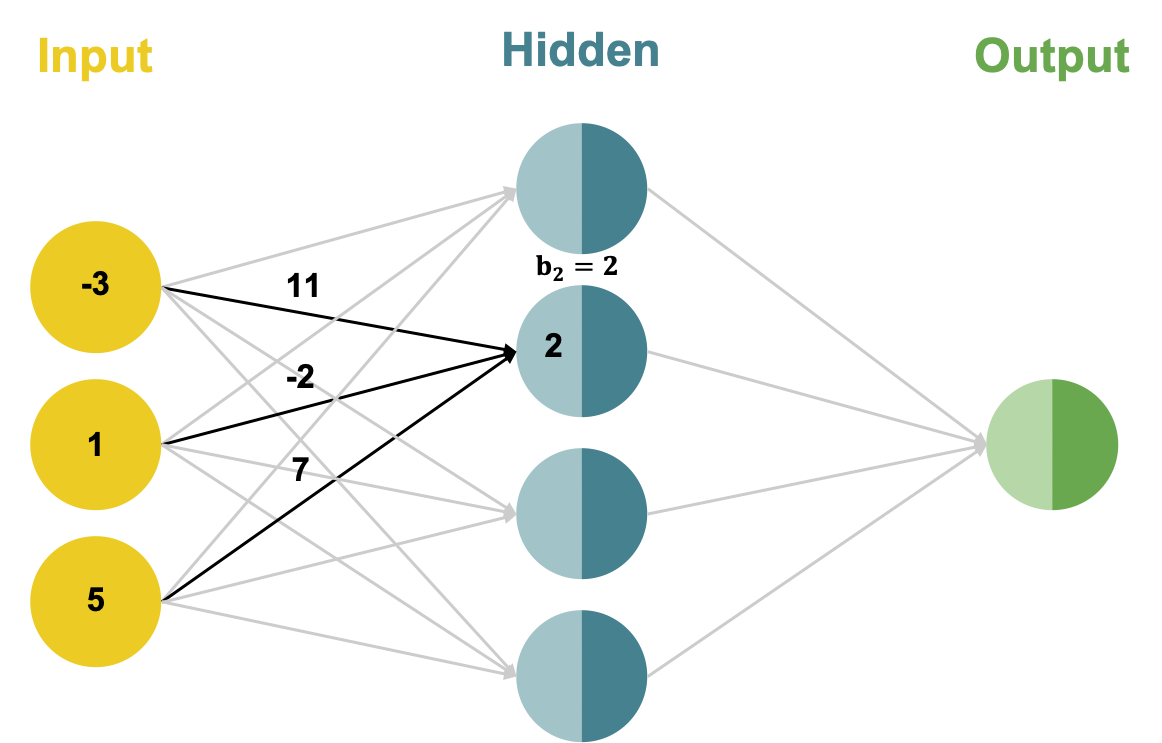
\includegraphics{figure/singlelay_2.png}} $$\begin{array}{l}
z_{\text {2,in}}=w_{12} x_1+w_{22} x_2+w_{32} x_3+b_2 \\
z_{\text {2,in}}= 11 * (-3) + (-2) * 1 + 7 * 5 + 2 = 2\end{array}$$}
\only<3>{\scalebox{.62}{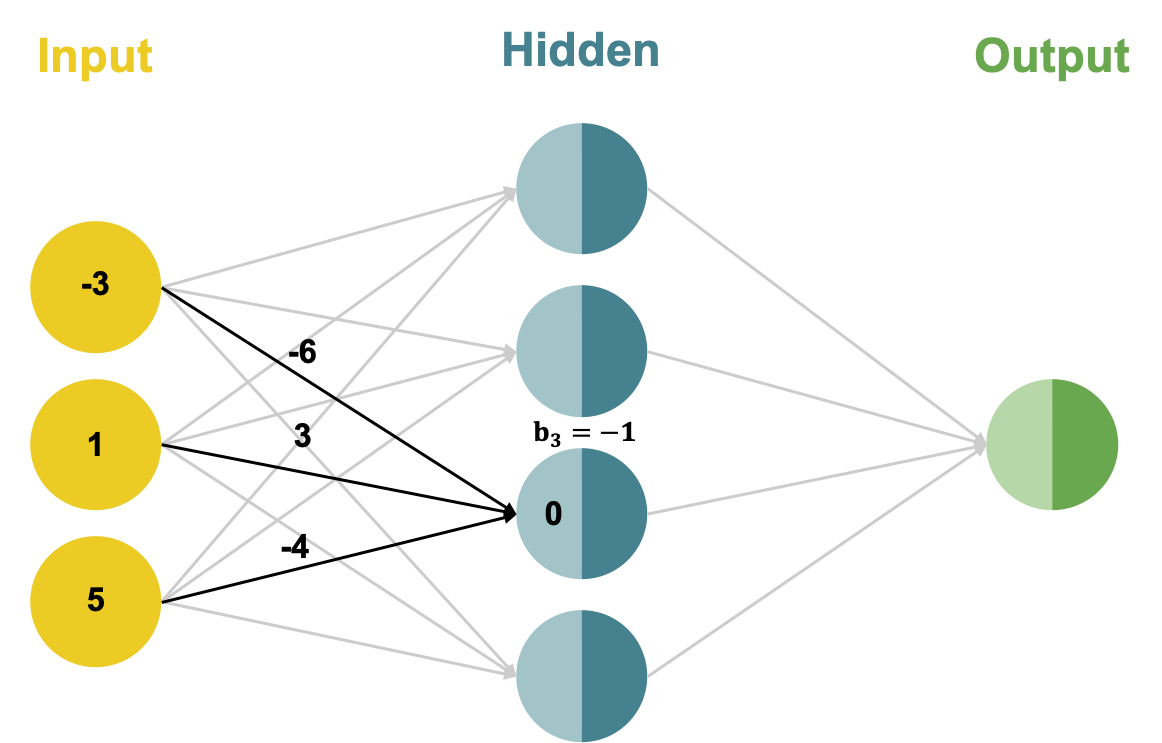
\includegraphics{figure/singlelay_3.png}}$$\begin{array}{l}
z_{\text {3,in}}=w_{13} x_1+w_{23} x_2+w_{33} x_3+b_3 \\
z_{\text {3,in}}= (-6) *(-3) + 3 * 1 + (-4) * 5 - 1 = 0\end{array}$$}
\only<4>{\scalebox{.62}{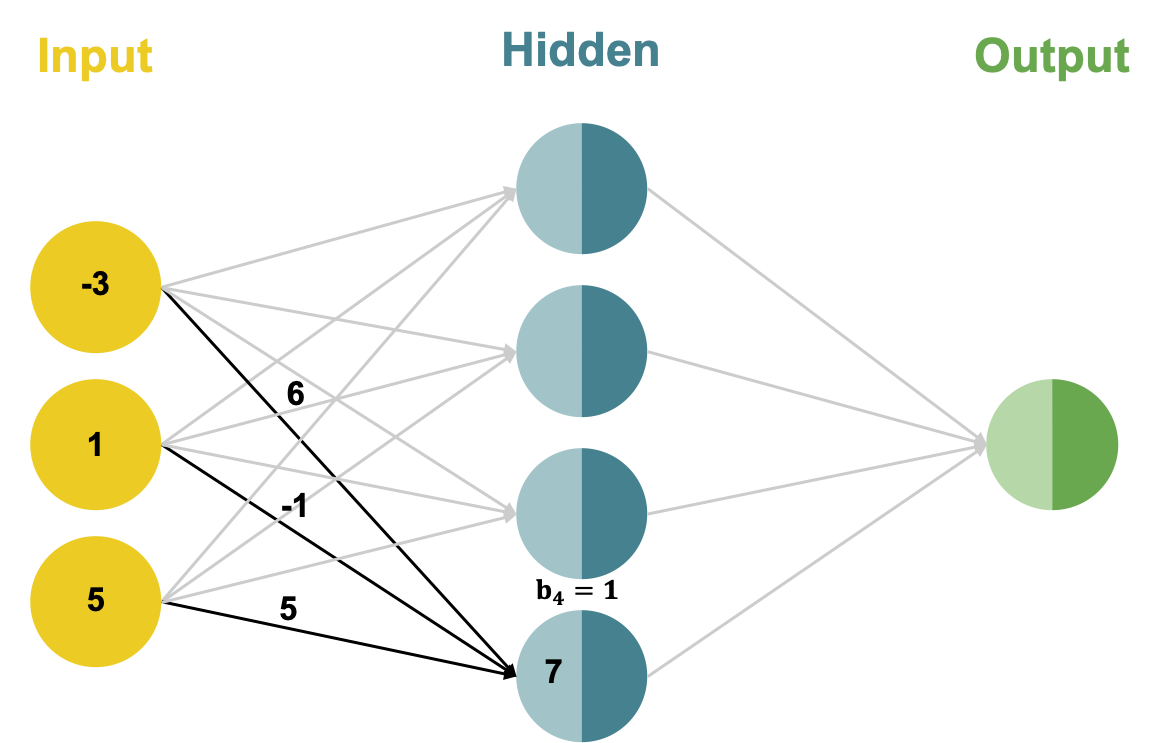
\includegraphics{figure/singlelay_4.png}}$$\begin{array}{l}
z_{\text {4,in}}=w_{14} x_1+w_{24} x_2+w_{34} x_3+b_4 \\
z_{\text {4,in}}= 6 * (-3) + (-1) * 1 + 5 * 5 + 1 = 7\end{array}$$}
\only<5>{\scalebox{.62}{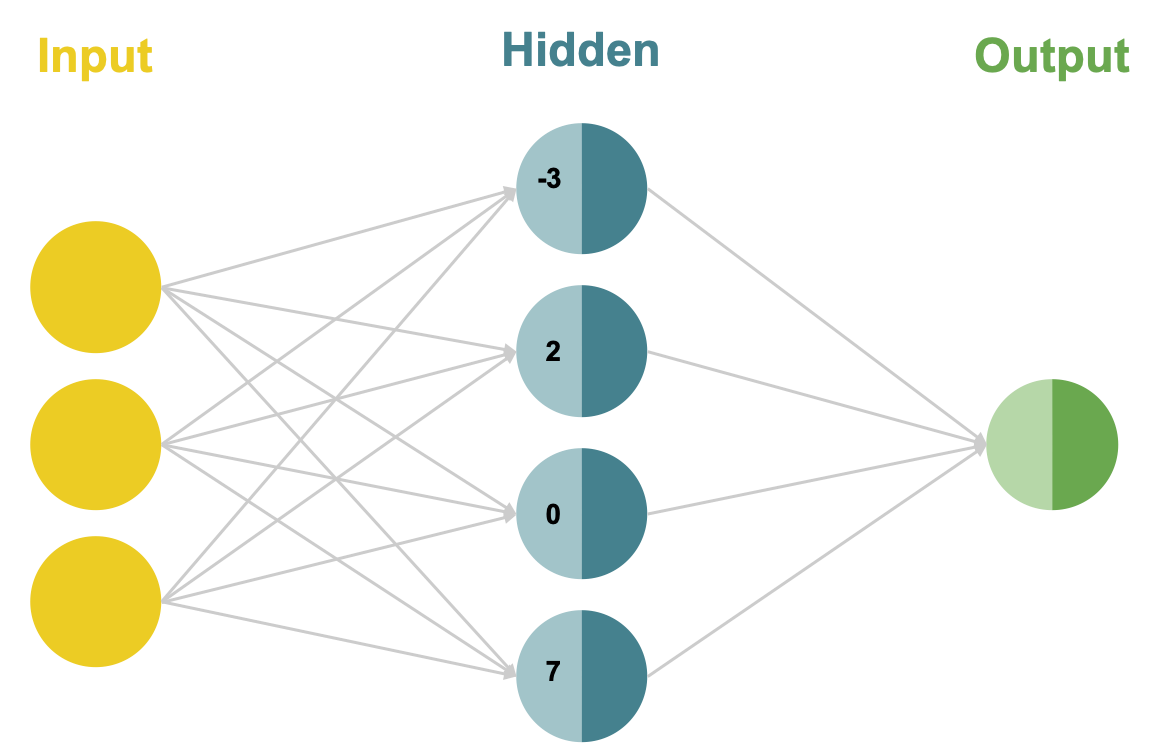
\includegraphics{figure/singlelay_5.png}}}
\end{figure}
\end{frame}

%%%%%%%%%%%%%%%%%%%%%%%%%%%%%%%%%%%%%%%%%%%%%%%%%%%%%%%%%%%%%%%%%%   1

\begin{frame} {Single Hidden Layer Networks: Example}
Each hidden neuron performs a non-linear \textbf{activation} transformation on the weight sum:
\begin{figure}
\centering
\only<1>{\scalebox{.62}{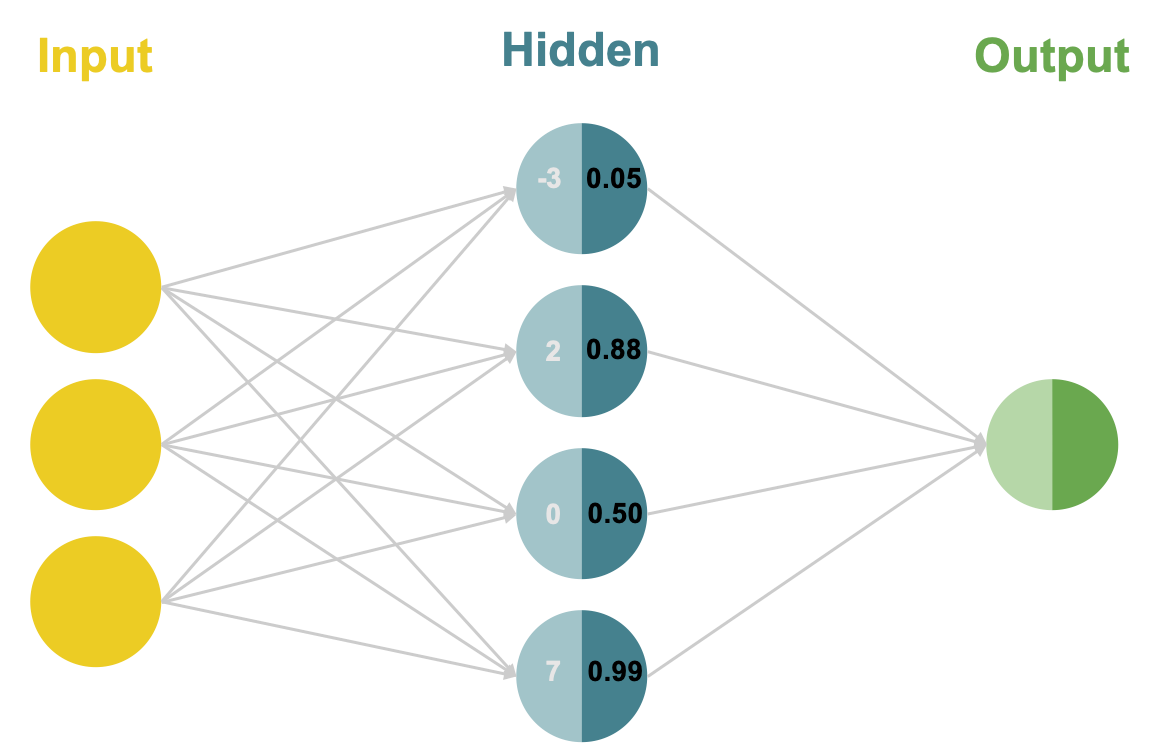
\includegraphics{figure/singlelay_6.png}}$$\begin{array}{l}
z_\text{i,out}=\sigma\left(z_{\text {i,in}}\right)=\frac{1}{1+e^{-z_{\text {in }}^{(i)}}}\end{array}$$}
\end{figure}
\end{frame}
%%%%%%%%%%%%%%%%%%%%%%%%%%%%%%%%%%%%%%%%%%%%%%%%%%%%%%%%%%%%%%%%%%  2

\begin{frame} {Single Hidden Layer Networks: Example}
The output neuron performs an \textbf{affine transformation} on its inputs:
\begin{figure}
\centering
\only<1>{\scalebox{.62}{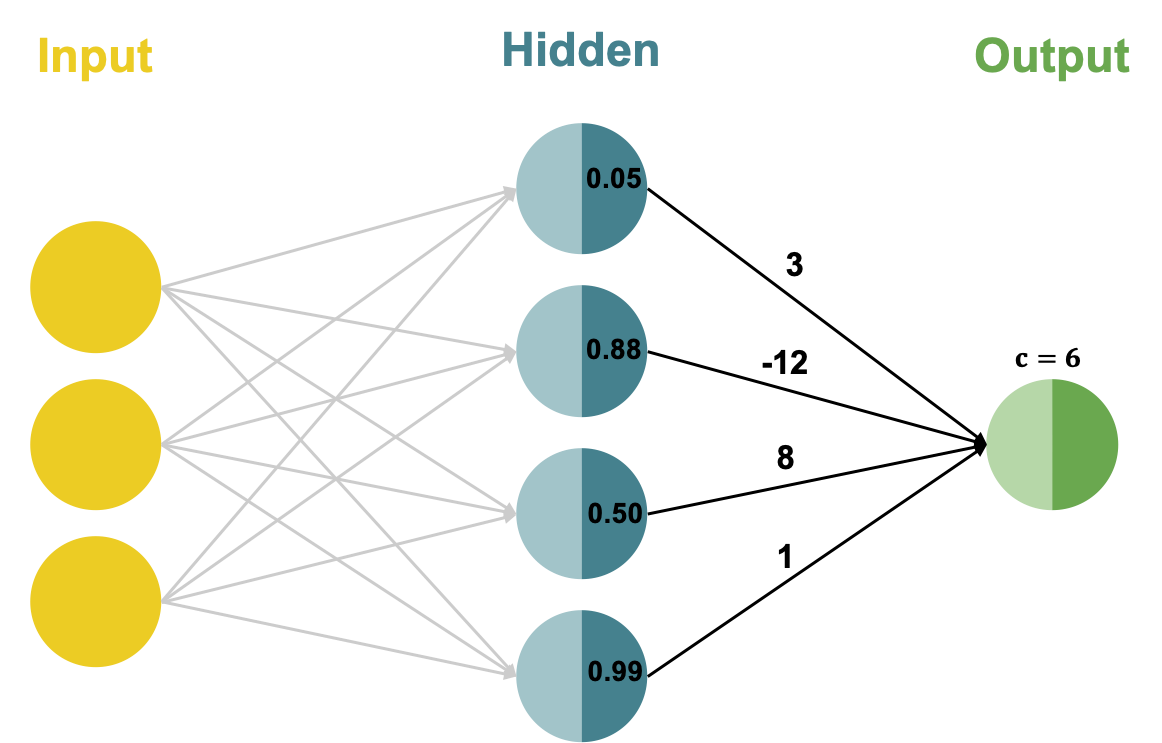
\includegraphics{figure/singlelay_7.png}}$$\begin{array}{l}
f_\text {in}=u_1 z_\text{1,out}+u_2 z_\text{2,out}+u_{3} z_\text{3,out}+u_{4} z_\text{4,out}+c\end{array}$$}
\only<2>{\scalebox{.62}{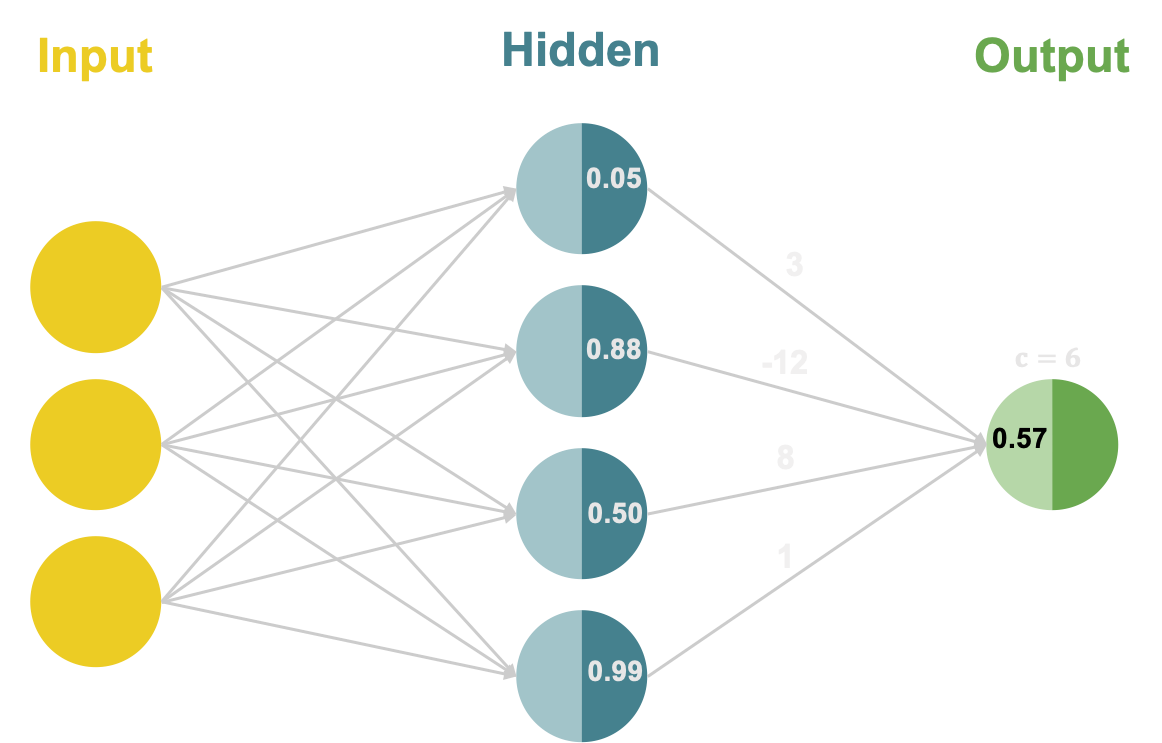
\includegraphics{figure/singlelay_8.png}}$$\begin{array}{l}
f_\text {in}=u_1 z_\text{1,out}+u_2 z_\text{2,out}+u_{3} z_\text{3,out}+u_{4} z_\text{4,out}+c \\ f_{\text {in}}= 3 * 0.05 + (-12) * 0.88 + 8* 0.50 + 1 * 0.99 + 6= 0.57\end{array}$$}
\end{figure}
\end{frame}
%%%%%%%%%%%%%%%%%%%%%%%%%%%%%%%%%%%%%%%%%%%%%%%%%%%%%%%%%%%%%%%%%%   1

\begin{frame} {Single Hidden Layer Networks: Example}
The output neuron performs a non-linear \textbf{activation} transformation on the weight sum:
\begin{figure}
\centering
\only<1>{\scalebox{.62}{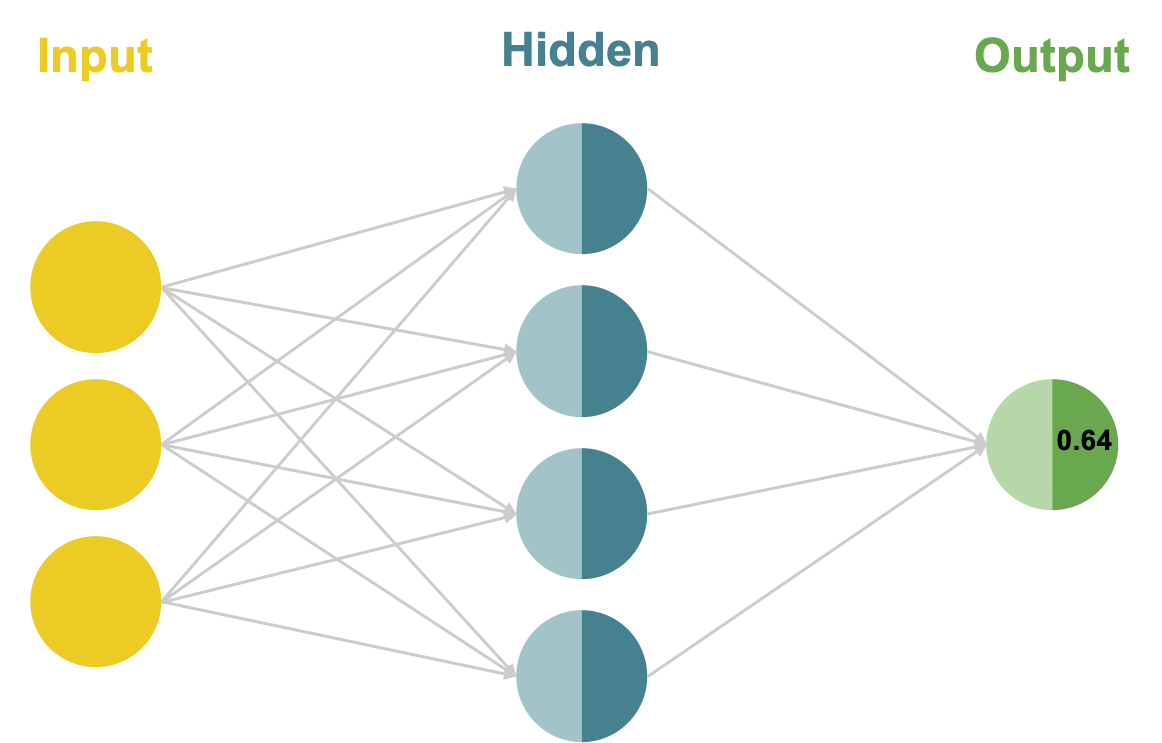
\includegraphics{figure/singlelay_9.png}}$$\begin{array}{l}
f_\text{out}=\sigma (f_\text{in})= \frac{1}{1+e^{-f_\text{in}}} \\ f_\text{out}=\frac{1}{1+e^{-0.57}}=0.64\end{array}$$}
\end{figure}
\end{frame}
%%%%%%%%%%%%%%%%%%%%%%%%%%%%%%%%%%%%%%%%%%%%%%%%%%%%%%%%%%%%%%%%%%
\begin{frame} {Hidden Layer: Activation Function}
\begin{itemize}
\item If the hidden layer does not have a non-linear activation, the network can only learn linear decision boundaries.
\item A lot of different activation functions exist.
%\item For simplification purposes, we drop the bias terms in notation and let $\sigma %= \text{id}$. Then:
 %   \begin{eqnarray*}
      % \fx & = & \tau(\\hidz) \\
      %   & = & \tau(\wtu^T \sigma(\Wmat^T \xv)) \\
      %  & = & \tau(\wtu^T\Wmat^T \xv) = \tau(\mathbf{v}^T \xv)
 %     \end{eqnarray*}
  %    where $ \mathbf{v} = \Wmat\wtu$. It can be seen that $\fx$ can only yield a linear decision boundary.
 \end{itemize}
\end{frame}


\begin{vbframe}{Hidden Layer: Activation Function}
%\textbf{Note:} if the hidden layer does not have a non-linear activation, the network can only learn linear decision boundaries.
\begin{blocki}{ReLU Activation:}
\item Currently the most popular choice is the ReLU (rectified linear unit):
$$ \sigma (v) = \max(0,v) $$
\end{blocki}
\begin{figure}
\scalebox{0.9}{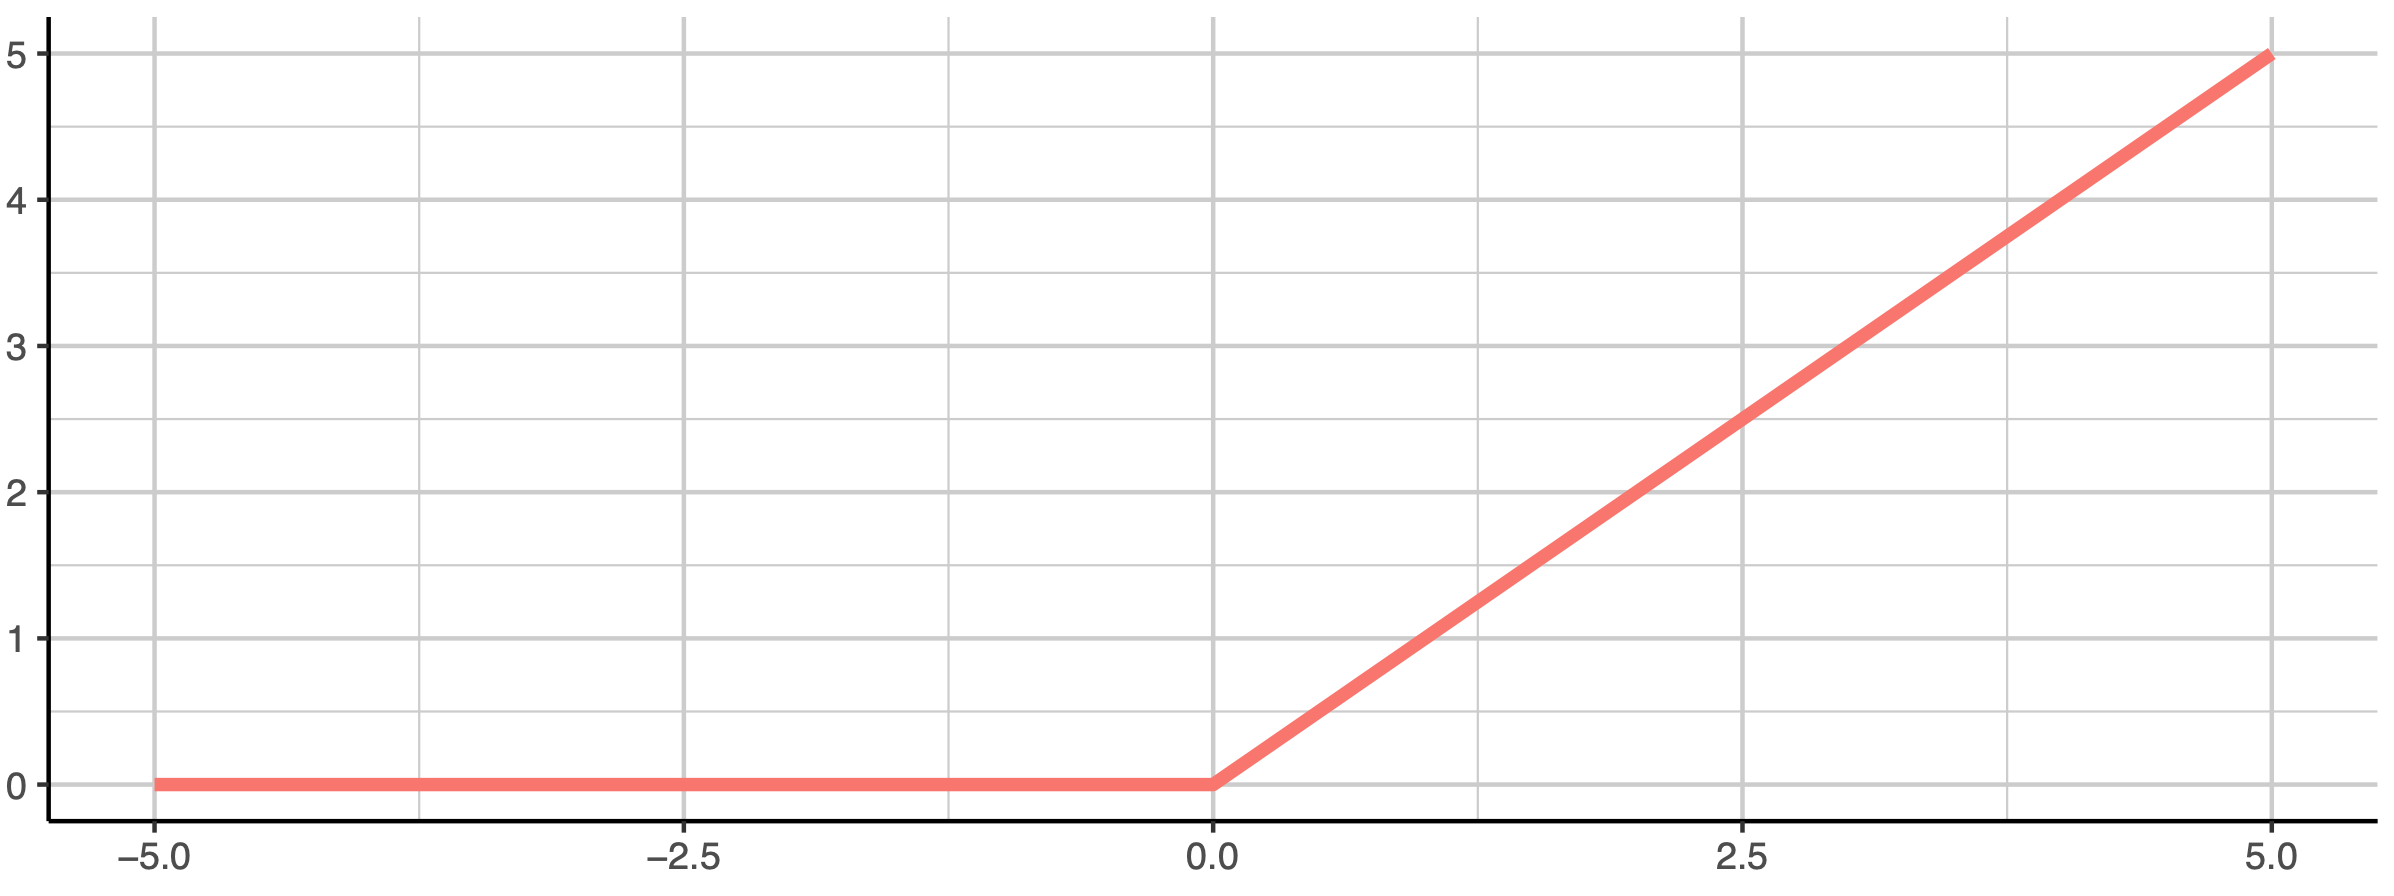
\includegraphics{figure/relu.png}}
\end{figure}
\framebreak
%%%%%%%%%%%%%%%%%%%%%%%%%%%%%%%%%%%%%%%%%%%%%%%%%%%%%%%%%%%%%%%%%%

%\begin{blocki}{Hyperbolic Tangent Activation:}
%\item Another choice might be the hyperbolic tangent function:
%$$ \sigma (v) = \text{tanh}(v) = \frac{\text{sinh}(v)}{\text{cosh}(v)} = 1 - \frac{2}{\exp(2v) + 1}$$
%\end{blocki}
%\begin{figure}
%\scalebox{0.9}{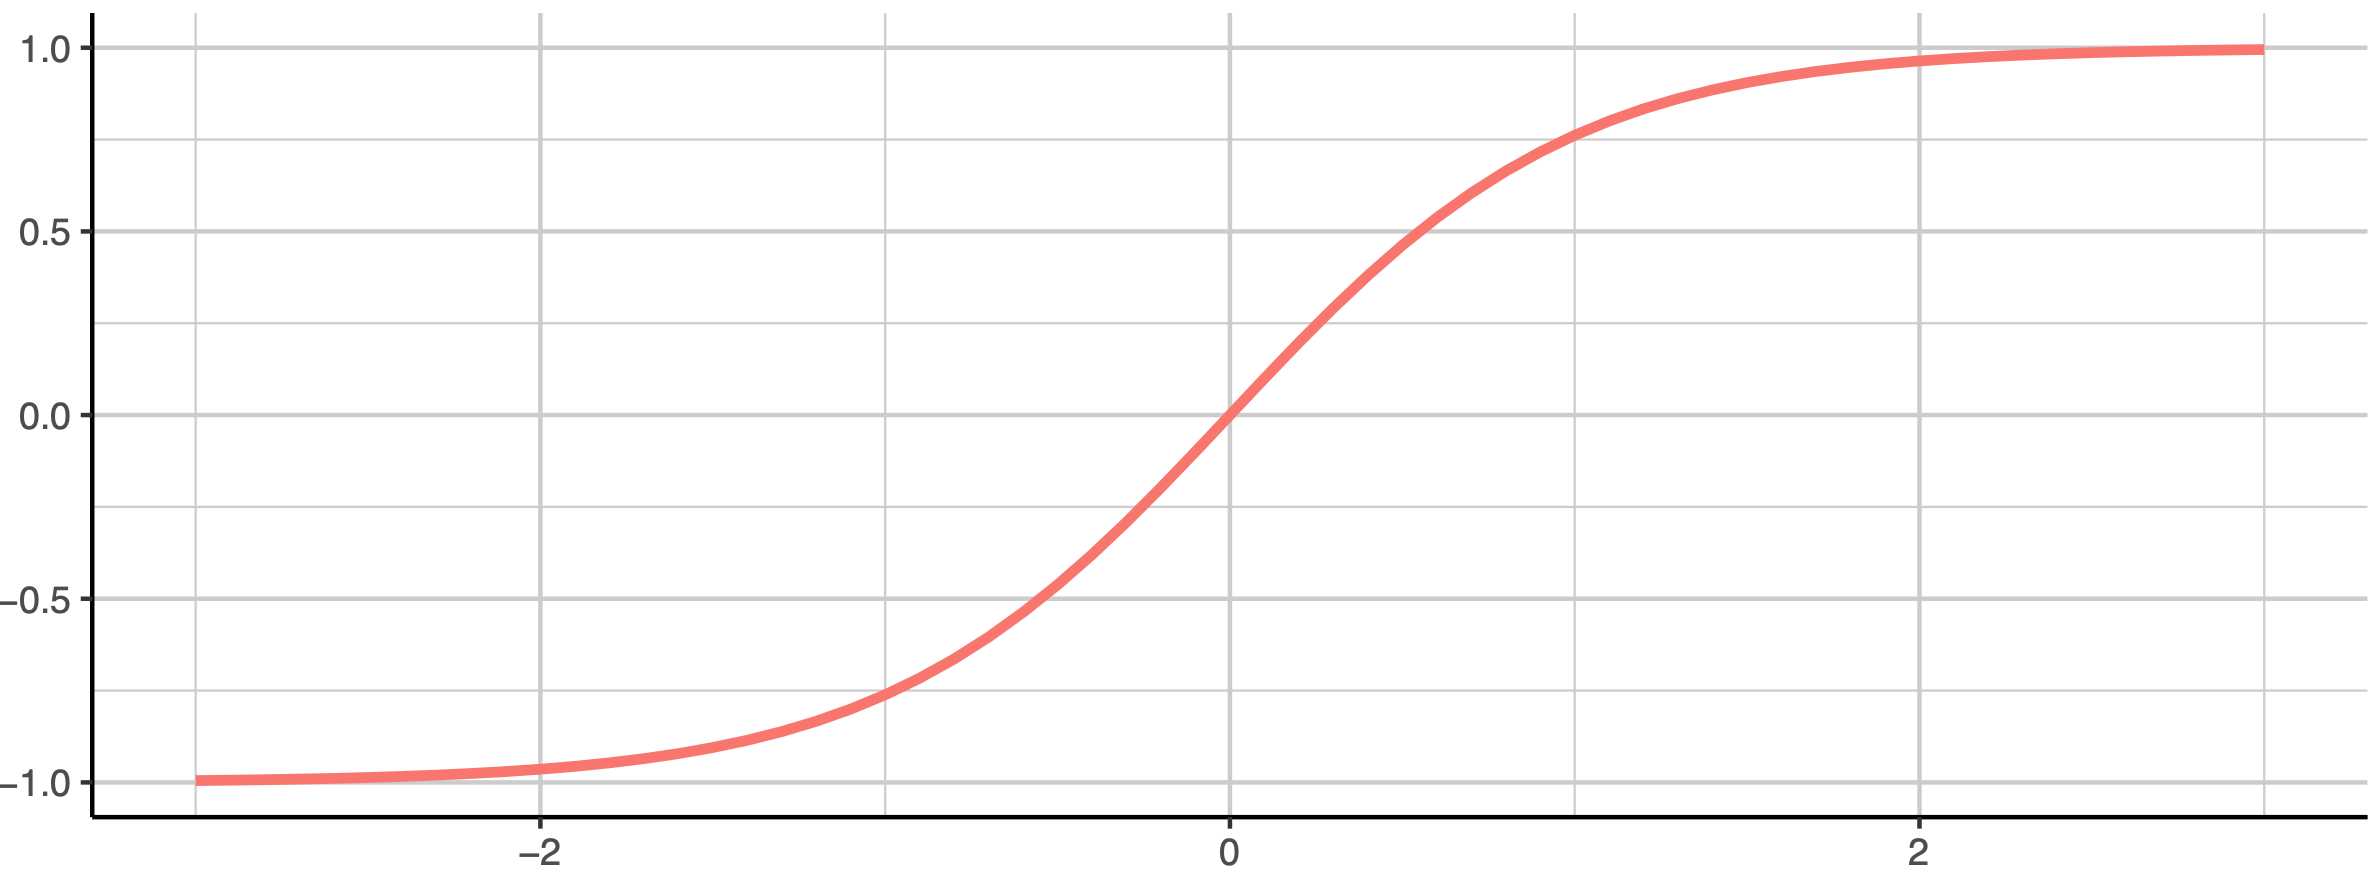
\includegraphics{figure/tanh.png}}
%\end{figure}
%\framebreak
%%%%%%%%%%%%%%%%%%%%%%%%%%%%%%%%%%%%%%%%%%%%%%%%%%%%%%%%%%%%%%%%%%

\begin{blocki}{Sigmoid Activation Function:}
\item The sigmoid function can be used even in the hidden layer:
$$ \sigma(v) = \frac{1}{1+\exp (-v)} $$
\end{blocki}
\begin{figure}
\scalebox{1}{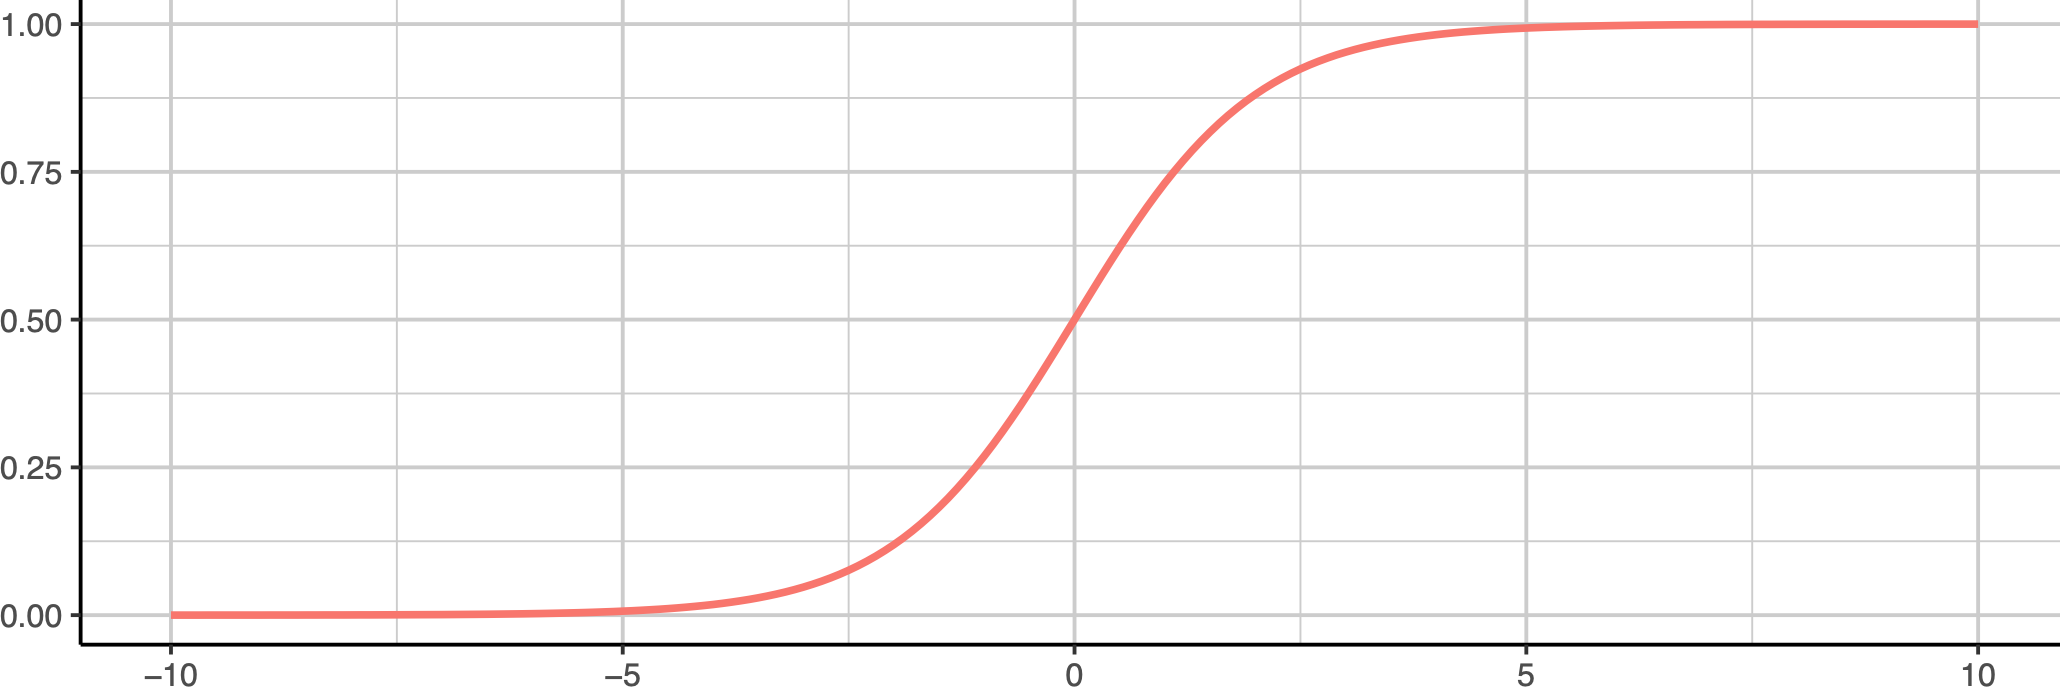
\includegraphics{figure/sigmoid.png}}
\end{figure}
\end{vbframe}

%%%%%%%%%%%%%%%%%%%%%%%%%%%%%%%%%%%%%%%%%%%%%%%%%%%


%%%%%%%%%%%%%%%%%%%%%%%%%%%%%%%%%%%%%%%%%%%%%%%%%%%%%%%%%%%%%%%%%%

%%%%%%%%%%%%%%%%%%%%%%%%%%%%%%%%%%%%%%%%%%%%%%%%%%%%%%%




\section{Matrix Notation}
%%%%%%%%%%%%%%%%%%%%%%%%%%%%%%%%%%%%%%%%%%%%%%%%%%%%%%%%%%%%%%%%%%

%\begin{frame}
%\frametitle{Lecture outline}
%\lz
%This chapter introduces a compact way for representing feedforward neural networks: the matrix formalism from linear algebra.
%\lz
%\lz
%
%\begin{enumerate}
%\item First, we explore networks with one hidden layer and one output unit.
%\lz
%\item Next, we investigate networks with one hidden layer but multiple output units.
%\lz
%\item Finally, we focus on multi-layer feedforward networks with an arbitrary number of hidden layers and output units.
%\end{enumerate}
%\end{frame}
%%%%%%%%%%%%%%%%%%%%%%%%%%%%%%%%%%%%%%%%%%%%%%%%%%%%%%%%%%%%%%%%%%%
%
%%\section{Single Hidden Layer Networks for Regression and Binary Classification}
%%%%%%%%%%%%%%%%%%%%%%%%%%%%%%%%%%%%%%%%%%%%%%%%%%%%%%%%%%%%%%%%%%%

\begin{vbframe}{Vectorized Notation: Hidden Layer}
\begin{itemize}
\item Input $\xv \in \R^{p \times 1}$, weight matrix $\Wmat \in \R^{p \times m}$ (one column per hidden neuron), bias $\biasb \in \R^{m \times 1}$.
\vspace{3mm}
\item All $m$ hidden neurons $z_1, \dots, z_m$ are computed at once:
$$ \hidz_{in} = \Wmat^T \xv + \biasb, \qquad \hidz = \sigma(\hidz_{in}) = \sigma(\Wmat^T \xv + \biasb),$$
where $\sigma$ is applied element-wise.
\vspace{3mm}
\item \textbf{Note}: The bias is often folded into $\Wmat$ by augmenting $\xv$ with a constant $1$; we won't draw it explicitly from here on.
\end{itemize}
\end{vbframe}
%%%%%%%%%%%%%%%%%%%%%%%%%%%%%%%%%%%%%%%%%%%%%%%%%%%%%%%%%%%%%%%%%%

\begin{vbframe}{Vectorized Notation: Output Layer}
\begin{itemize}
  \vspace{4mm}
  \item For regression or binary classification: one output unit $f$ where
    \begin{itemize}
      \item $f_{in} = \wtu^T \hidz + c$ , i.e. a linear combination of derived features plus the bias term $c$ of the output neuron, and
      \vspace{2mm}
      \item $\fx= f_{out} = \tau(f_{in}) = \tau(\wtu^T \hidz + c)$ , where $\tau$ is the output activation function.
    \end{itemize}
  \item For regression $\tau$ is the identity function; for binary classification, $\tau$ is a sigmoid function.
  \item \textbf{Note}: $\sigma$ introduces the non-linearities that let the network learn complex functions; $\tau$ merely rescales the final score to match the target's range.
\end{itemize}
\end{vbframe}
%%%%%%%%%%%%%%%%%%%%%%%%%%%%%%%%%%%%%%%%%%%%%%%%%%%%%%%%%%%%%%%%%%

\begin{vbframe}{Vectorized Notation: Batched Inputs}
\begin{itemize}
\item Multiple inputs $\xi$, $i \in \nset$, are stacked as rows of a \textbf{design matrix} $\Xmat \in \R^{n \times p}$.
\vspace{2mm}
\item Hidden activations for the whole batch, computed at once:
$$\bm{Z} = \sigma(\Xmat\Wmat + \bm{B}) \in \R^{n \times m},$$
where $\bm{B}$ duplicates $\biasb$ as the rows of an ($n \times m$) matrix.
\vspace{2mm}
\item Final output for the whole batch:
$$\tau(\bm{Z}\wtu + \bm{C}) \in \R^{n \times 1},$$
where $\bm{C}$ duplicates the scalar bias $c$ as the rows of an ($n \times 1$) matrix.
\end{itemize}
\end{vbframe}
%%%%%%%%%%%%%%%%%%%%%%%%%%%%%%%%%%%%%%%%%%%%%%%%%%%%%%%%%%%%%%%%%%%

\section{The XOR Problem}

\begin{vbframe}{Example: XOR Problem}
  \begin{itemize}
    \item Suppose we have four data points $$X = \{(0,0)^\top, (0,1)^\top, (1,0)^\top, (1,1)^\top \}$$
    \item The XOR gate (exclusive or) returns true, when an odd number of inputs are true:
  \end{itemize}
  \begin{table}
    \centering
      \begin{tabular}{ccc}
        \textbf{$x_1$}  & \textbf{$x_2$}  & \textbf{XOR} $= y$ \\
        \hline
        \hline
        $0$             &   $0$           &  $0$ \\
        $0$             &   $1$           &  $1$ \\
        $1$             &   $0$           &  $1$ \\
        $1$             &   $1$           &  $0$
      \end{tabular}
  \end{table}
  \begin{itemize}
    \item Can you learn the target function with a logistic regression model? \\
    % (Aside from statistical generalization, we just want to learn the training data!)
  \end{itemize}
\framebreak
  \begin{minipage}{0.45\textwidth}
    \begin{itemize}
      \item Logistic regression can not solve this problem. %and will always output $0.5$. \\
      In fact, any model using simple hyperplanes for separation can not (including a single neuron).
      \lz
      \item A small neural net can easily solve the problem by transforming the space!
    \end{itemize}
  \end{minipage}
  \begin{minipage}{0.5\textwidth}
    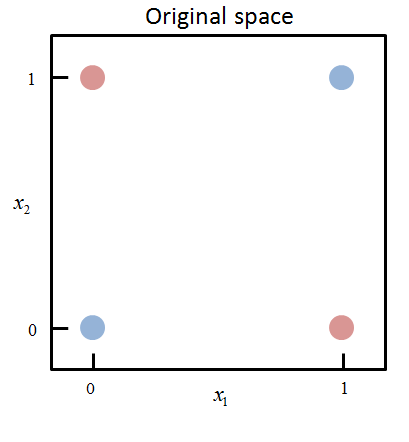
\includegraphics{figure/xor1.png}%
  \end{minipage}\hfill
\framebreak
  \begin{itemize}
    \item Consider the following model:
  \end{itemize}
    \begin{figure}
      \centering
        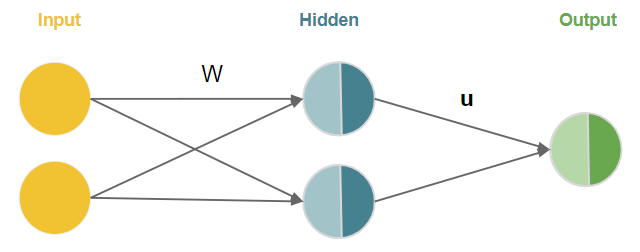
\includegraphics[width=8cm]{figure/xor_rep.png}%
        \caption{A neural network with two neurons in the hidden layer. The matrix $\Wmat$ describes the mapping from $\xv$ to $\hidz$. The vector $\wtu$ from $\hidz$ to $y$.}
    \end{figure}
\framebreak
  \begin{itemize}
    \item Let use ReLU $\sigma(z) = \max\left\{0, z \right\}$ as activation function and a simple thresholding function $\tau(z) = [ z > 0 ] =  \begin{cases} 1 & \text{ if } z > 0 \\ 0 & \text{otherwise} \end{cases} $ \\ as output transformation function. We can represent the architecture of the model by the following equation: 
  \end{itemize}
  \begin{eqnarray*}
    f(\xv~|~ \Wmat, \biasb, \wtu, \biasc) &=&  \tau\left(\wtu^\top\sigma(\Wmat^\top \xv+\biasb)+\biasc\right) \\
                &=& \tau\left(\wtu^\top \max\{0, \Wmat^\top \xv+\biasb\} + \biasc\right)
  \end{eqnarray*}
  % \begin{footnotesize}
  % \textbf{Note:} To simplify calculations, we \enquote{falsely} treat the problem as a regression problem (no final output transformation $\tau$ to map scores to $[0, 1]$). We will see later that transformation to $[0, 1]$ is not necessary in this very special case.
  % \end{footnotesize}
  \begin{itemize}
    \item So how many parameters does our model have?
    \begin{itemize}
      \item In a fully connected neural net, the number of connections between the nodes equals our parameters: $$\underbrace{(2 \times 2)}_{W} + \underbrace{(2 \times 1)}_{\biasb} + \underbrace{(2 \times 1)}_{\wtu} + \underbrace{(1)}_{c} = 9$$
    \end{itemize}
  \end{itemize}
\framebreak
  \begin{eqnarray*}
   \text{Let} \ \Wmat = \begin{pmatrix}
      1 & 1 \\
      1 & 1
    \end{pmatrix}, \
      \biasb = \begin{pmatrix}
      0 \\
      -1
    \end{pmatrix}, \
      \wtu = \begin{pmatrix}
      1 \\
      -2
    \end{pmatrix}, \
      c = - 0.5
  \end{eqnarray*}
  \begin{eqnarray*}
    \Xmat = \begin{pmatrix}
      0 & 0 \\
      0 & 1 \\
      1 & 0 \\
      1 & 1
    \end{pmatrix}, \
    \Xmat \Wmat = \begin{pmatrix}
      0 & 0 \\
      1 & 1 \\
      1 & 1 \\
      2 & 2
    \end{pmatrix}, \
      \Xmat \Wmat + \bm{B} = \begin{pmatrix}
        0 & -1 \\
        1 & 0 \\
        1 & 0 \\
        2 & 1
    \end{pmatrix}
  \end{eqnarray*}
%\vspace{4mm}
 \footnotesize{Note: $\Xmat$ is a $(n \times p)$ design matrix in which the \textit{rows} correspond to the data points. $\Wmat$, as usual, is a $(p \times m)$ matrix where each \textit{column} corresponds to a single (hidden) neuron. $\bm{B}$ is a ($n \times m$) matrix with $\biasb$ duplicated along the rows.}
 \begin{figure}
    \centering
      \scalebox{0.6}{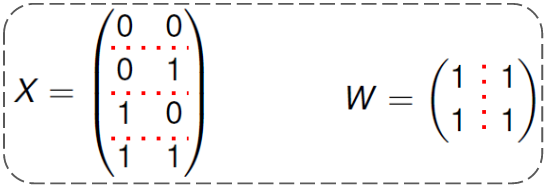
\includegraphics{figure/rowcol.png}}
  \end{figure}
 \framebreak
 \normalsize{
 \begin{eqnarray*}
   \text{Let} \ \Wmat = \begin{pmatrix}
      1 & 1 \\
      1 & 1
    \end{pmatrix}, \
      \biasb = \begin{pmatrix}
      0 \\
      -1
    \end{pmatrix}, \
      \wtu = \begin{pmatrix}
      1 \\
      -2
    \end{pmatrix}, \
      c = - 0.5
  \end{eqnarray*}
  \begin{eqnarray*}
  \Xmat = \begin{pmatrix}
      0 & 0 \\
      0 & 1 \\
      1 & 0 \\
      1 & 1
    \end{pmatrix}, \
    \Xmat\Wmat = \begin{pmatrix}
      0 & 0 \\
      1 & 1 \\
      1 & 1 \\
      2 & 2
    \end{pmatrix}, \
      \Xmat \Wmat + \bm{B} = \begin{pmatrix}
        0 & -1 \\
        1 & 0 \\
        1 & 0 \\
        2 & 1
    \end{pmatrix}
  \end{eqnarray*}
  \begin{eqnarray*}
    \bm{Z} = \max\{0, \Xmat \Wmat+\bm{B}\}
    &=&
    \begin{pmatrix}
      0 & 0 \\
      1 & 0 \\
      1 & 0 \\
      2 & 1
    \end{pmatrix}
  \end{eqnarray*}
  \begin{itemize}
    \item Note that we computed all examples at once.
  \end{itemize}

\framebreak
  \begin{minipage}{0.45\textwidth}
    \begin{itemize}
      \item The input points are mapped into transformed space to
        \begin{eqnarray*}
          \bm{Z} = \begin{pmatrix}
              0 & 0 \\
              1 & 0 \\
              1 & 0 \\
              2 & 1
          \end{pmatrix}
        \end{eqnarray*}
    %  \item[] which is easily separable.
    \end{itemize}
  \end{minipage}
  \begin{minipage}{0.5\textwidth}
    \includegraphics<1>{figure/xor2_2.png}%
  \end{minipage}\hfill
  
\framebreak
  \begin{minipage}{0.45\textwidth}
    \begin{itemize}
      \item The input points are mapped into transformed space to
        \begin{eqnarray*}
          \bm{Z} = \begin{pmatrix}
              0 & 0 \\
              1 & 0 \\
              1 & 0 \\
              2 & 1
          \end{pmatrix}
        \end{eqnarray*}
      \item[] which is easily separable.
    \end{itemize}
  \end{minipage}
  \begin{minipage}{0.5\textwidth}
    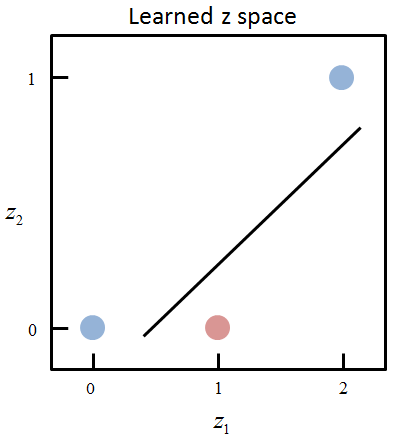
\includegraphics{figure/xor2.png}%
  \end{minipage}\hfill
  
\framebreak
  \begin{itemize}
    \item In a final step we have to multiply the activated values of matrix $\bm{Z}$ with the vector $\wtu$ and add the bias term $c$:
  \end{itemize}
  \begin{eqnarray*}
    f(\xv ~|~ \Wmat, \biasb, \wtu, c) &=&
    \begin{pmatrix}
      0 & 0 \\
      1 & 0 \\
      1 & 0 \\
      2 & 1
    \end{pmatrix}
    \begin{pmatrix}
      1 \\
      -2
    \end{pmatrix} + 
    \begin{pmatrix}
      - 0.5 \\
      - 0.5 \\
      - 0.5 \\
      - 0.5
    \end{pmatrix}
    =
    \begin{pmatrix}
      - 0.5 \\
      0.5 \\
      0.5 \\
      - 0.5
    \end{pmatrix}
  \end{eqnarray*}
  \begin{itemize}
    \item And then apply the step function $\tau(z) = [z > 0 ]$.  This solves the XOR problem perfectly!
  \end{itemize}
  \begin{table}
    \centering
      \begin{tabular}{ccc}
        \textbf{$x_1$}  & \textbf{$x_2$}  & \textbf{XOR} = y\\
        \hline
        \hline
        $0$             &   $0$           &  $0$ \\
        $0$             &   $1$           &  $1$ \\
        $1$             &   $0$           &  $1$ \\
        $1$             &   $1$           &  $0$
      \end{tabular}
  \end{table}
  }
\end{vbframe}



\begin{frame} {Neural Networks : Optimization}
  \begin{itemize}
    \item In this simple example we actually \enquote{guessed} the values of the parameters for $\textbf{W}$, $\biasb$, $\wtu$ and $c$.
    \vspace{3mm}
    \item That won't work for more sophisticated problems!
    \vspace{3mm}
    %\item To learn the right weights (and biases), we once again have to rely on iterative algorithms like gradient descent.
    \item We will learn later about iterative optimization algorithms for automatically adapting weights and biases.
    \vspace{3mm}
    \item An added complication is that the loss function is no longer convex. Therefore, there might not exist a single minimum. 
    %Therefore, gradient descent can only find a local minimum. 
 %   \vspace{3mm}
  %  \item An extremely efficient method to compute gradients called backpropogation will be covered in the next lecture.
  \end{itemize}
\end{frame}


\section{Multi-Class Classification}

%%%%%%%%%%%%%%%%%%%%%%%%%%%%%%%%%%%%%%%%%%%%%%%%%%%%%%%%%%%%%%%%%%
%\section{Single Hidden Layer Networks for Multi-Class Classification}
%%%%%%%%%%%%%%%%%%%%%%%%%%%%%%%%%%%%%%%%%%%%%%%%%%%%%%%%%%%%%%%%%%

\begin{frame} {Multi-class Classification}
\vspace{20mm}
\begin{itemize}
\item We have only considered regression and binary classification problems so far.
\vspace{5mm}
\item How can we get a neural network to perform multiclass classification?
  \end{itemize}
\end{frame}
%%%%%%%%%%%%%%%%%%%%%%%%%%%%%%%%%%%%%%%%%%%%%%%%%%%%%%%%%%%%%%%%%%

\begin{frame} {Multi-class Classification}
\begin{itemize}
\item The first step is to add additional neurons to the output layer.
\item Each neuron in the layer will represent a specific class (number of neurons in the output layer = number of classes).
\begin{figure}
\centering
\scalebox{0.6}{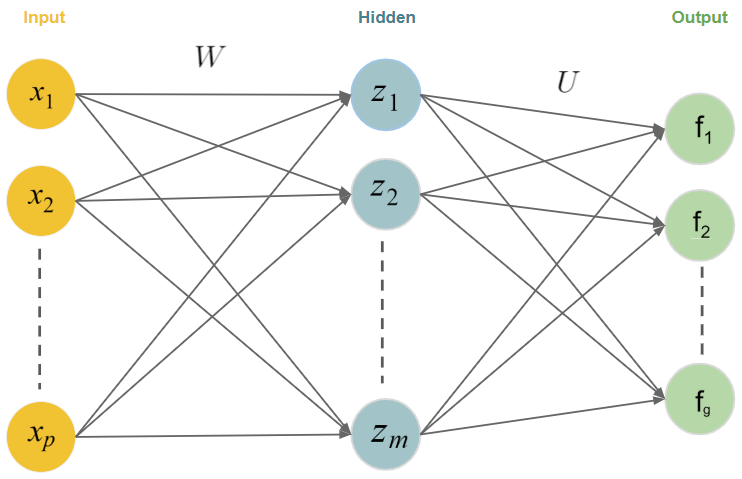
\includegraphics[width=10.2cm]{figure/neuralnet_new.png}}
\caption{\footnotesize Structure of a single hidden layer, feed-forward neural network for g-class classification problems (bias term omitted).}
\end{figure}
\end{itemize}
\end{frame}
%%%%%%%%%%%%%%%%%%%%%%%%%%%%%%%%%%%%%%%%%%%%%%%%%%%%%%%%%%%%%%%%%%

\begin{frame} {Multi-class Classification}
\vspace{5mm}
\begin{blocki}{Notation:}
\item For $g$-class classification, $g$ output units: $$\mathbf{f} = (f_1, \dots, f_g)$$
%\vspace{4mm}
\item $m$ hidden neurons $z_1, \dots, z_m$, with
    $$ z_j = \sigma(\mathbf{W}_j^T \xv), \quad j = 1,\ldots,m. $$
\item Compute linear combinations of derived features $z$:
    $$ f_{in,k} = \bm{U}_k^T \hidz, \quad \hidz=(z_1,\dots, z_m)^T, \quad k = 1,\ldots,g$$
\end{blocki}
\end{frame}
%%%%%%%%%%%%%%%%%%%%%%%%%%%%%%%%%%%%%%%%%%%%%%%%%%%%%%%%%%%%%%%%%%

\begin{frame} {Multi-class Classification}
  \begin{itemize}
    \item The second step is to apply a \textbf{softmax} activation function to the output layer.
    \vspace{4mm}
    \item This gives us a probability distribution over $g$ different possible classes:
    $$ f_{out,k} = \tau_k(f_{in,k}) = \frac{\exp(f_{in,k})}{\sum_{k'=1}^g\exp(f_{in,k'})}$$
    \vspace{2mm}
    \item This is the same transformation used in softmax regression!
    \vspace{4mm}
    \item Derivative $ \frac{\partial \tau(\mathbf{f}_{in})}{\partial \mathbf{f}_{in}} = \text{diag}(\tau(\mathbf{f}_{in})) - \tau(\mathbf{f}_{in}) \tau(\mathbf{f}_{in})^T $
    \vspace{4mm}
    \item It is a \enquote{smooth} approximation of the argmax operation,
        so $\tau((1, 1000, 2)^T) \approx (0, 1, 0)^T$ (picks out 2nd element!).
  \end{itemize}
\end{frame}
%%%%%%%%%%%%%%%%%%%%%%%%%%%%%%%%%%%%%%%%%%%%%%%%%%%%%%%%%%%%%%%%%%

\begin{frame} {Multi-class Classification: Example}
Forward pass (Hidden: Sigmoid, Output: Softmax).
  \begin{figure}
    \centering
      \only<1>{\scalebox{0.72}{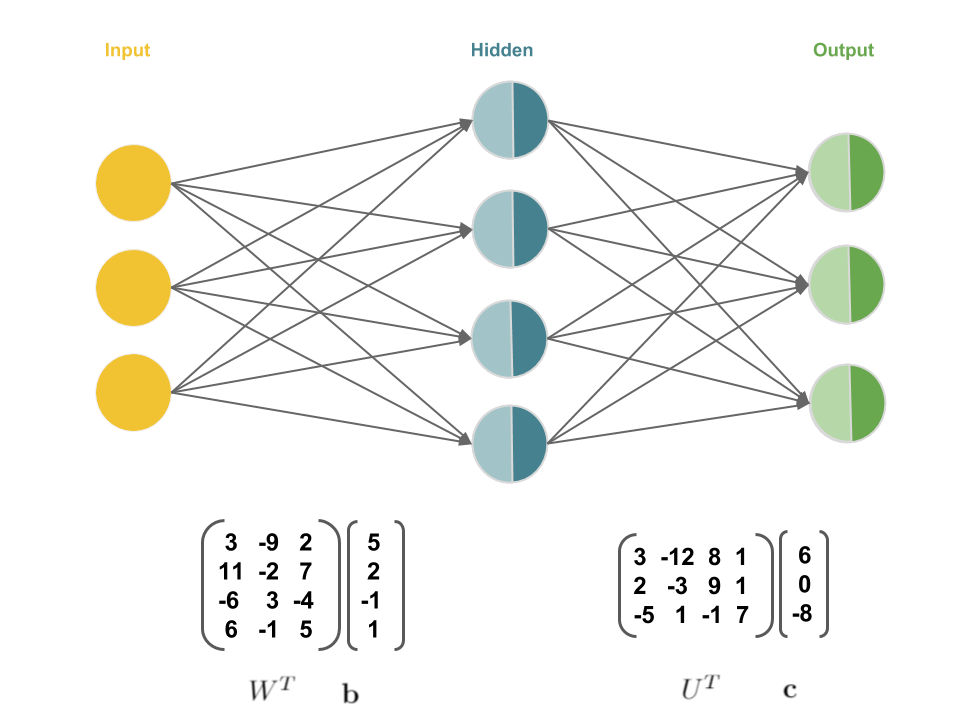
\includegraphics{figure/softie_one.png}}}
      \only<2>{\scalebox{0.72}{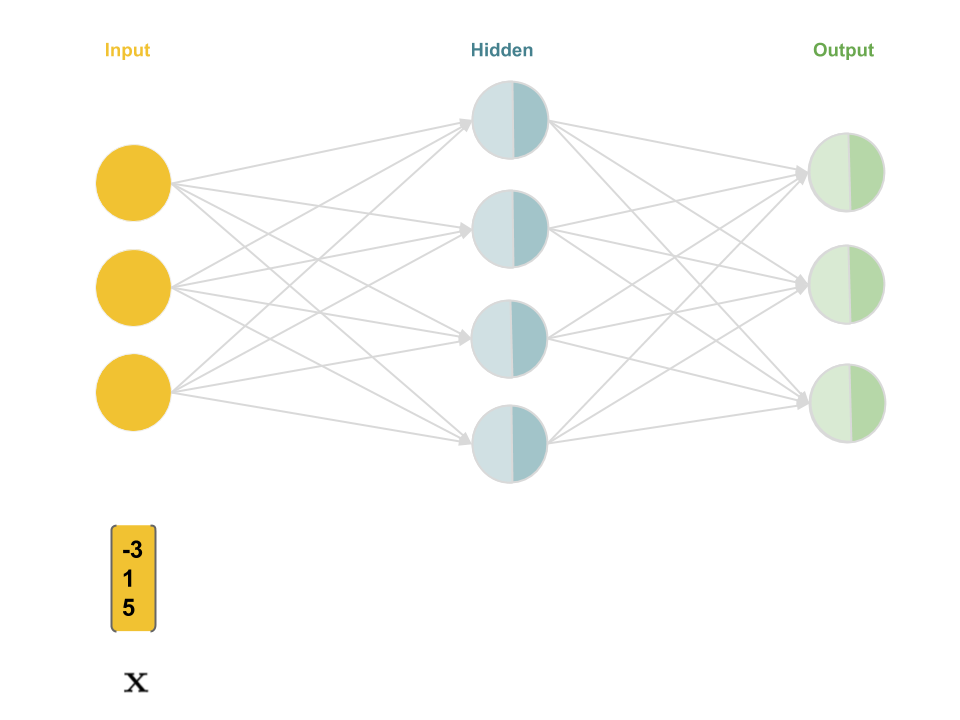
\includegraphics{figure/softie_two.png}}}
      \only<3>{\scalebox{0.72}{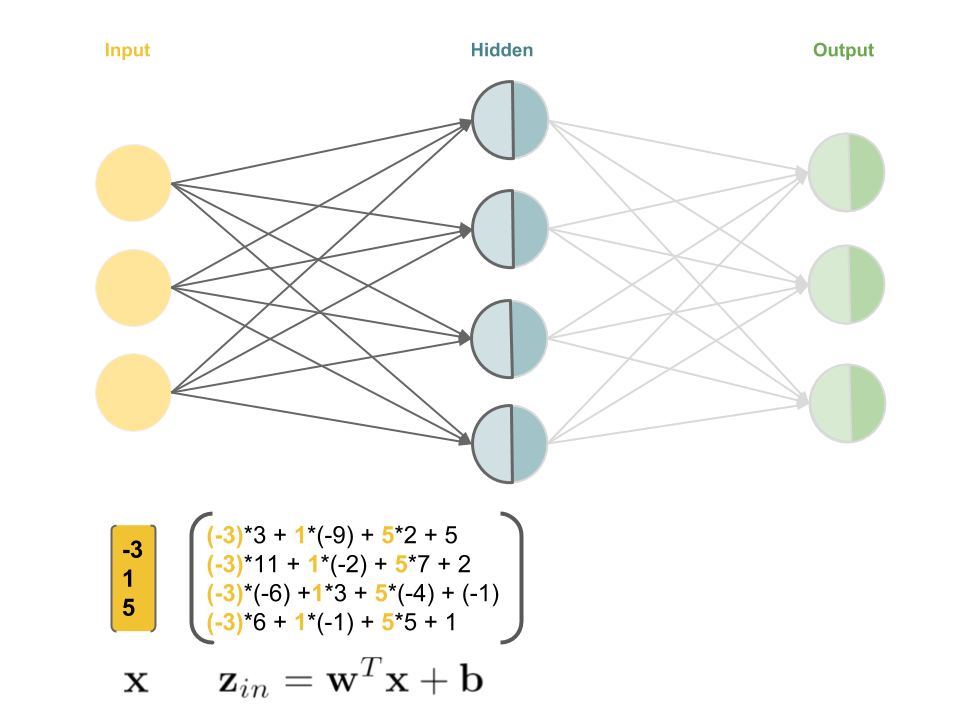
\includegraphics{figure/softie_three.png}}}
      \only<4>{\scalebox{0.72}{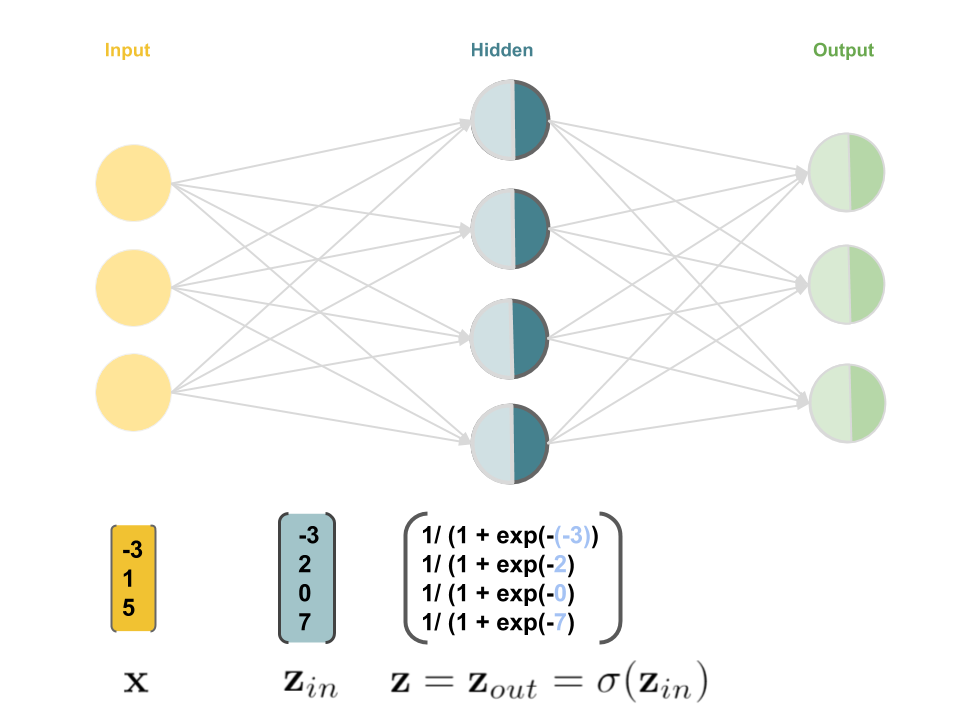
\includegraphics{figure/softie_four.png}}}
      \only<5>{\scalebox{0.72}{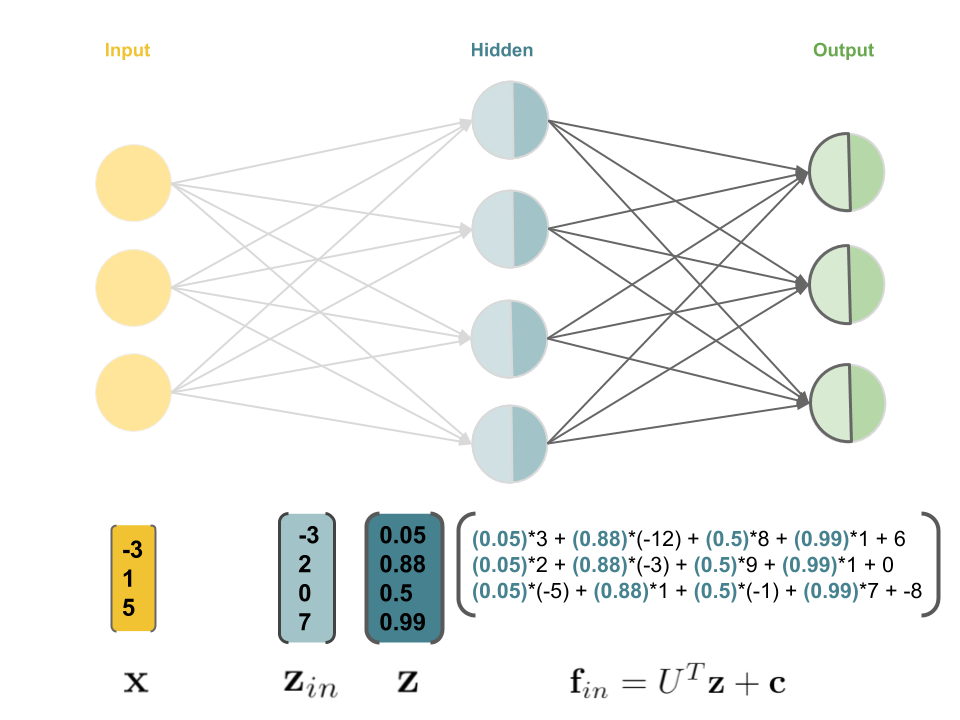
\includegraphics{figure/softie_five_a.png}}}
      \only<6>{\scalebox{0.72}{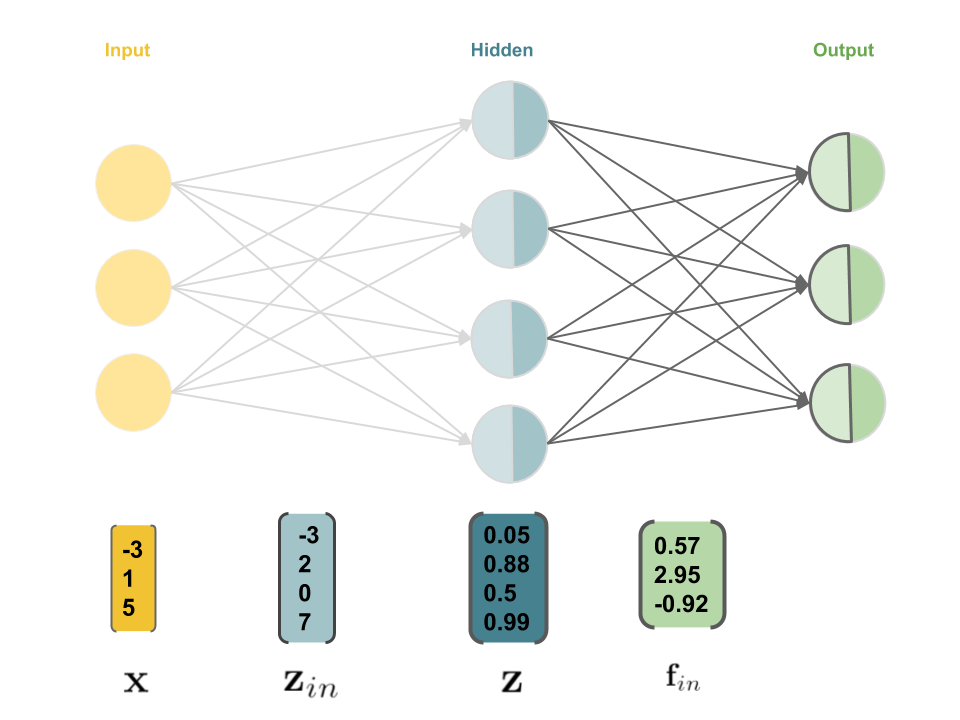
\includegraphics{figure/softie_five_b.png}}}
      \only<7>{\scalebox{0.72}{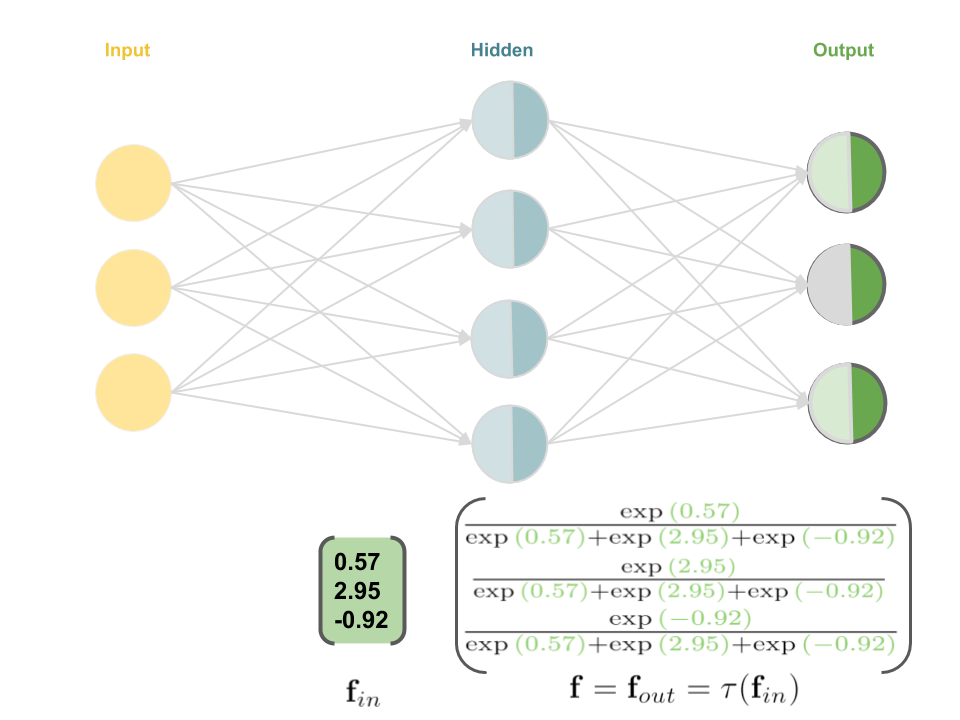
\includegraphics{figure/softie_six.png}}}
      \only<8>{\scalebox{0.72}{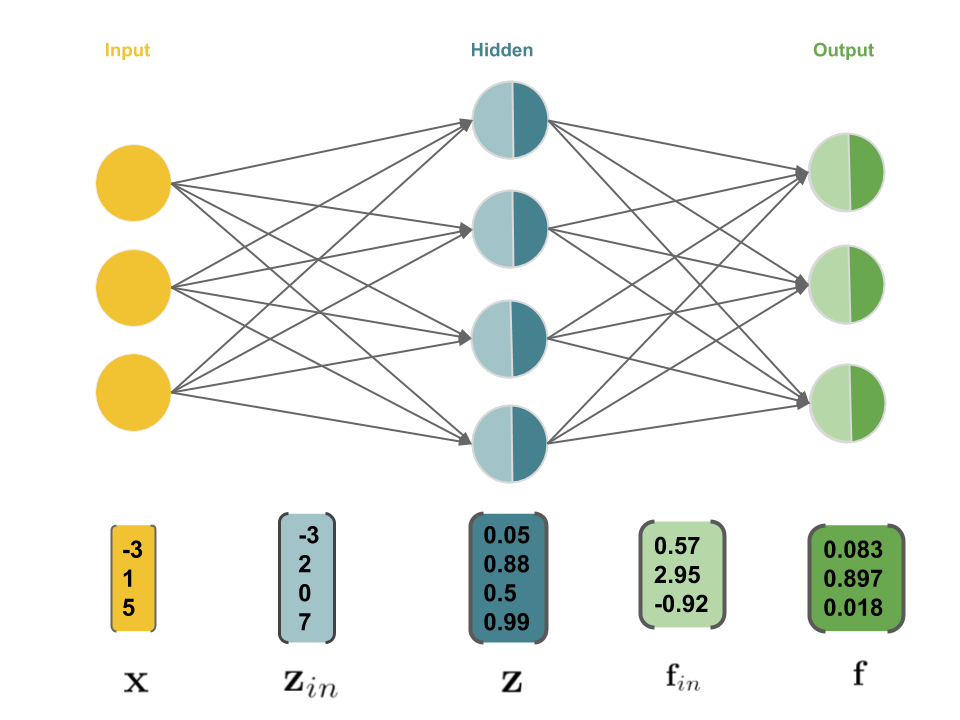
\includegraphics{figure/softie_seven.png}}}
\end{figure}
\end{frame}
%%%%%%%%%%%%%%%%%%%%%%%%%%%%%%%%%%%%%%%%%%%%%%%%%%%%%%%%%%%%%%%%%%

\begin{frame} {Optimization: Softmax Loss}
  \begin{itemize}
\vspace{5mm}
\item The loss function for a softmax classifier is
$$L(y, \fx) = - \sum_{k = 1}^g [y = k] \log \left( \frac{\exp(f_{in,k})}{\sum_{k'=1}^g\exp(f_{in,k'})}\right)$$
where $[y = k] = \begin{cases} 1 & \text{ if } y = k \\
0 & \text{ otherwise }
\end{cases}$. 
\vspace{5mm}
\item This is equivalent to the cross-entropy loss when the label vector $\bm{y}$ is one-hot coded (e.g. $\mathbf{y} = (0,0,1,0)^T$). 
\item Optimization:  Again, there is no analytic solution.
\end{itemize}
\end{frame}
%%%%%%%%%%%%%%%%%%%%%%%%%%%%%%%%%%%%%%%%%%%%%%%%%%%%%%%%%%%%%%%%%%


\section{Multi-Layer Feedforward Neural Networks}


%\section{Multi-Layer Feedforward Neural Networks}
%%%%%%%%%%%%%%%%%%%%%%%%%%%%%%%%%%%%%%%%%%%%%%%%%%%%%%%%%%%%%%%%%%

\begin{vbframe}{Feedforward neural networks}
\begin{itemize}
\vspace{15mm}
\item We will now extend the model class once again, such that we allow an arbitrary amount $l$ of hidden layers.
\vspace{5mm}
\item The general term for this model class is (multi-layer) \textbf{feedforward networks} (inputs are passed through the network from left to right, no feedback-loops are allowed)
\end{itemize}
\framebreak
%%%%%%%%%%%%%%%%%%%%%%%%%%%%%%%%%%%%%%%%%%%%%%%%%%%%%%%%%%%%%%%%%%

\begin{itemize}
\item We can characterize those models by the following chain structure: $$f = \tau \circ \phi \circ \sigma^{(l)} \circ \phi^{(l)} \circ \sigma^{(l-1)} \circ \phi^{(l-1)} \circ \ldots \circ \sigma^{(1)} \circ \phi^{(1)}$$ where $\sigma^{(i)}$ and $\phi^{(i)}$ are the activation function and the weighted sum of hidden layer $i$, respectively. $\tau$ and $\phi$ are the corresponding components of the output layer.
\vspace{5mm}
\item Each hidden layer has: 
\begin{itemize}
\vspace{2mm}
\item an associated weight matrix $\Wmat^{(i)}$, bias $\biasb^{(i)}$, and activations $\hidz^{(i)}$ for $i \in \{ 1 \ldots l\}$.
\vspace{2mm}
\item $\hidz^{(i)} = \sigma^{(i)}(\phi^{(i)}) = \sigma^{(i)}(\Wmat^{(i)T}\hidz^{(i - 1)} + \biasb^{(i)})$ , where $\hidz^{(0)} = \xv$.
\end{itemize}
\vspace{5mm}
\item Again, without non-linear activations in the hidden layers, the network can only learn linear decision boundaries.
  \end{itemize}
\framebreak
%%%%%%%%%%%%%%%%%%%%%%%%%%%%%%%%%%%%%%%%%%%%%%%%%%%%%%%%%%%%%%%%%%

\lz
\begin{figure}
\centering
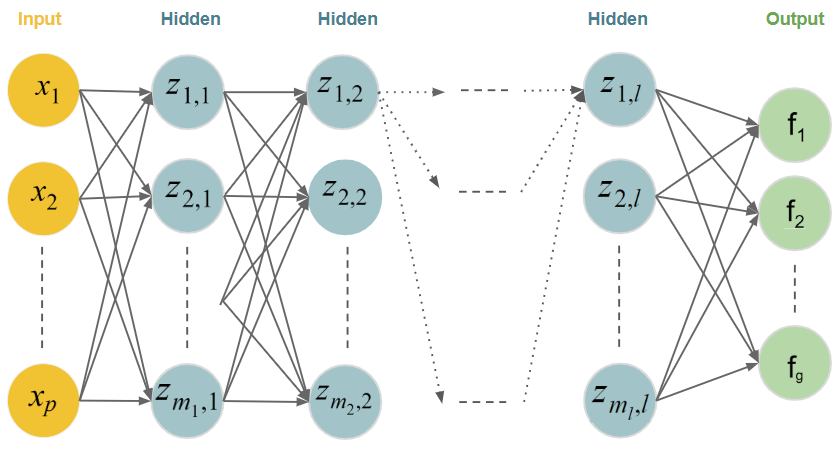
\includegraphics[width=10.5cm]{figure/deepneuralnet_new.png}
\caption{Structure of a deep neural network with $l$ hidden layers (bias terms omitted).}
  \end{figure}
\end{vbframe}  
%%%%%%%%%%%%%%%%%%%%%%%%%%%%%%%%%%%%%%%%%%%%%%%%%%%%%%%%%%%%%%%%%%

\begin{frame} {Feedforward neural networks: Example}
\begin{figure}
\centering
\only<1>{\scalebox{0.8}{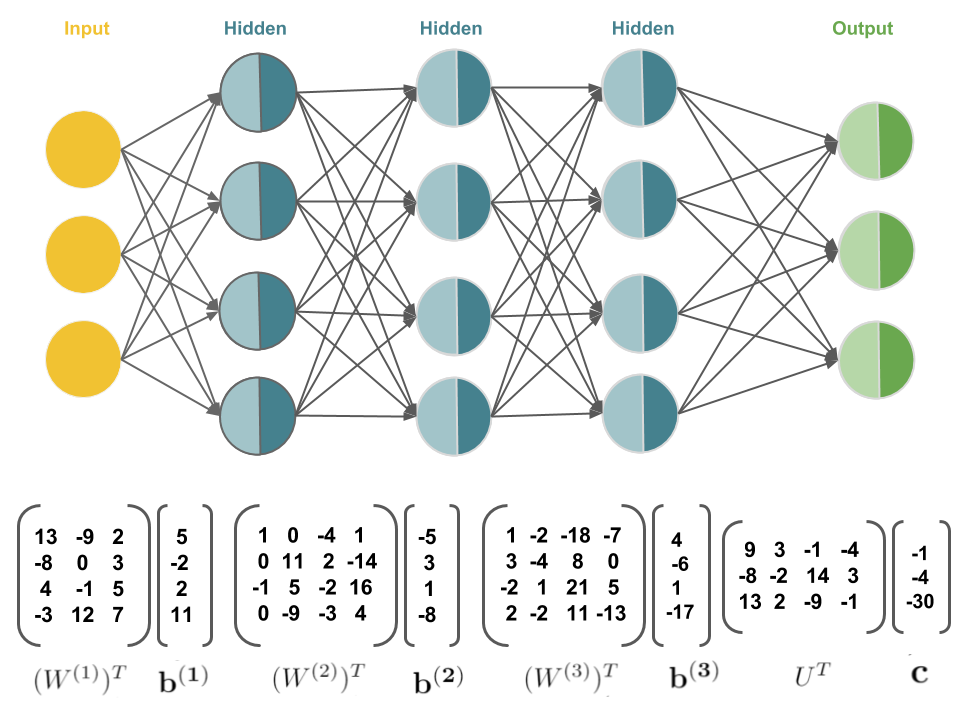
\includegraphics{figure/deepnet_one.png}}}
\only<2>{\scalebox{0.8}{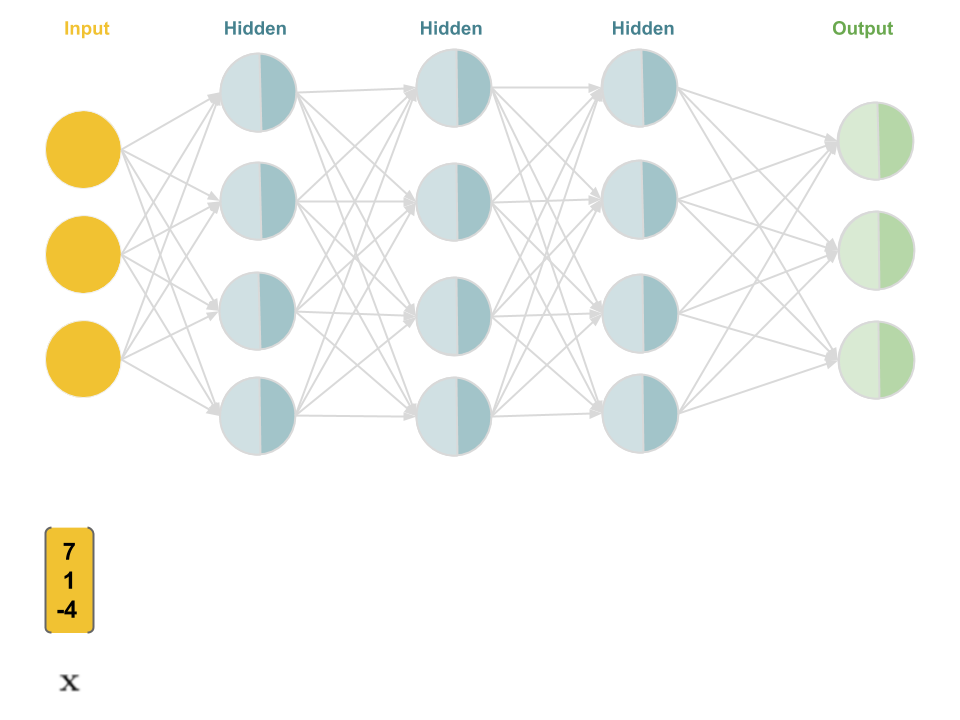
\includegraphics{figure/deepnet_two.png}}}
\only<3>{\scalebox{0.8}{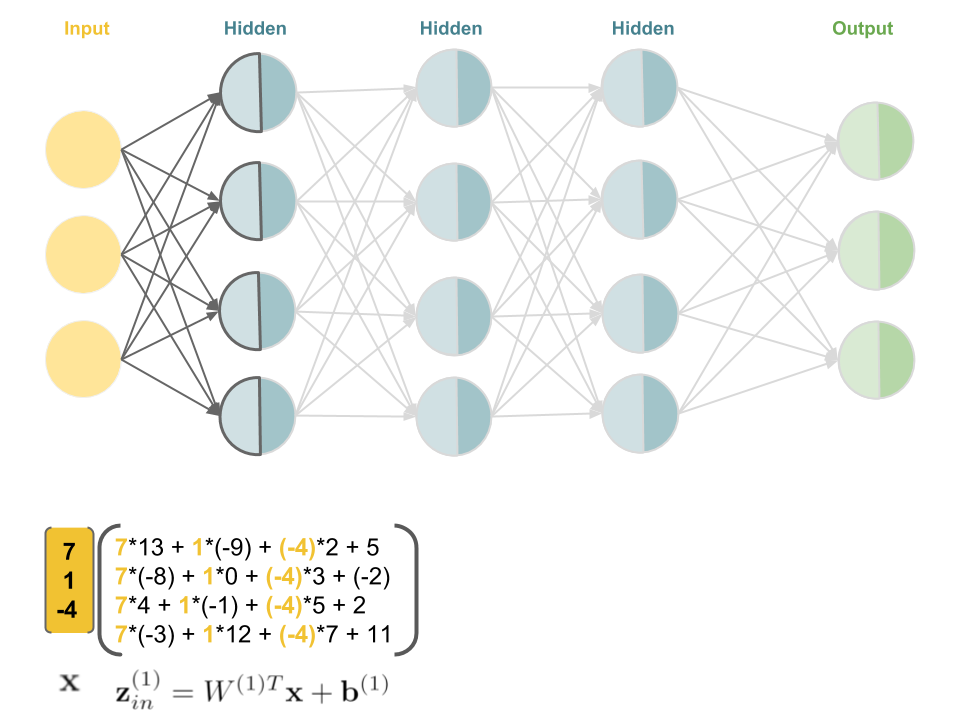
\includegraphics{figure/deepnet_three.png}}}
\only<4>{\scalebox{0.8}{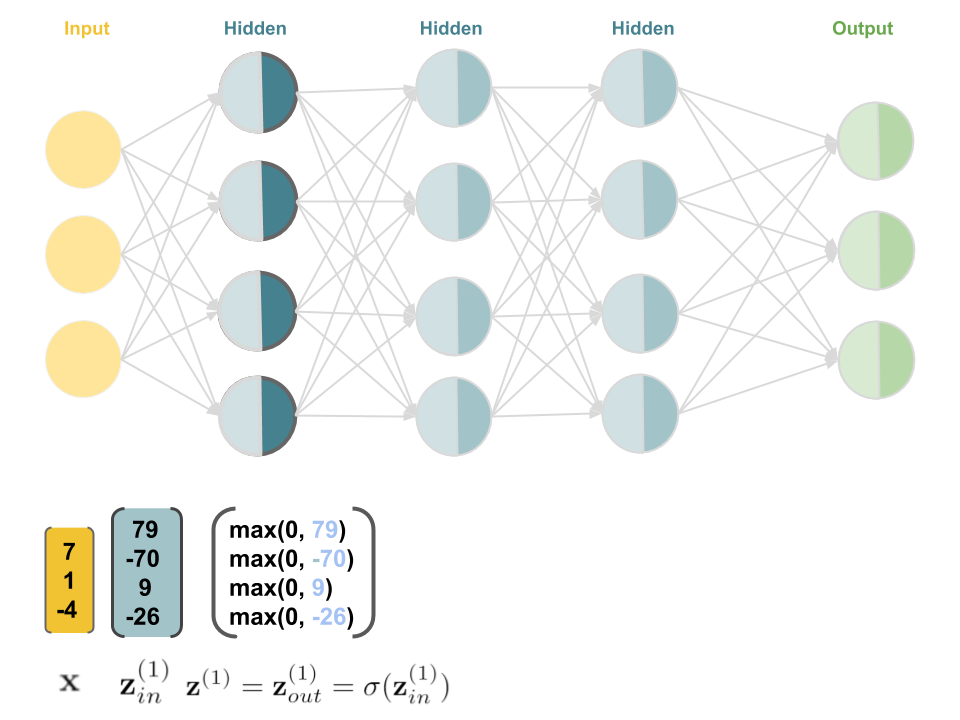
\includegraphics{figure/deepnet_four.png}}}
\only<5>{\scalebox{0.8}{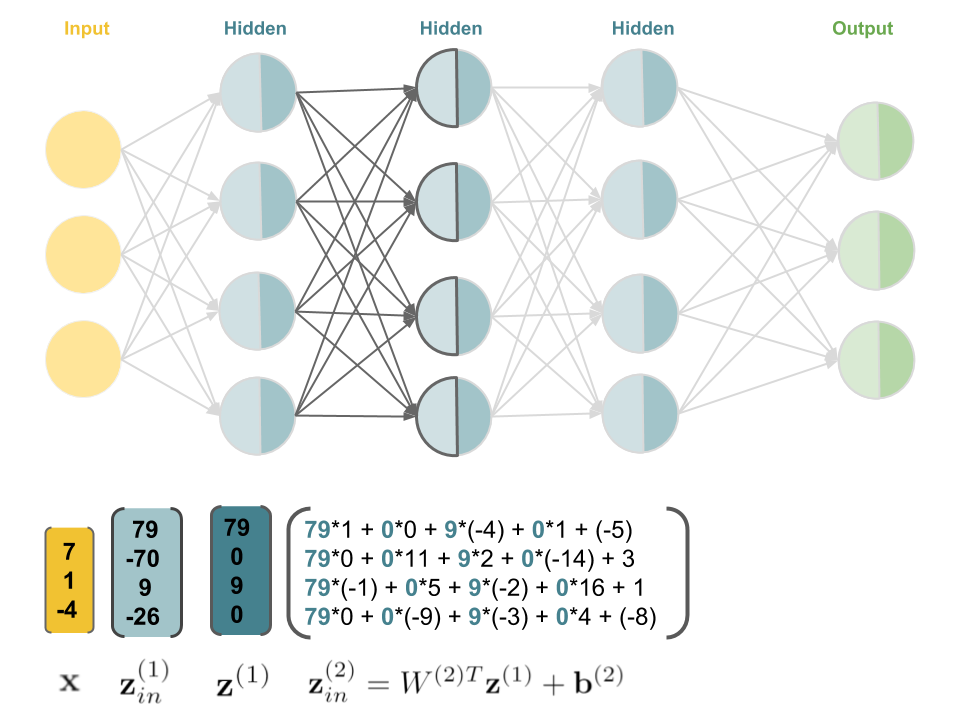
\includegraphics{figure/deepnet_five.png}}}
\only<6>{\scalebox{0.8}{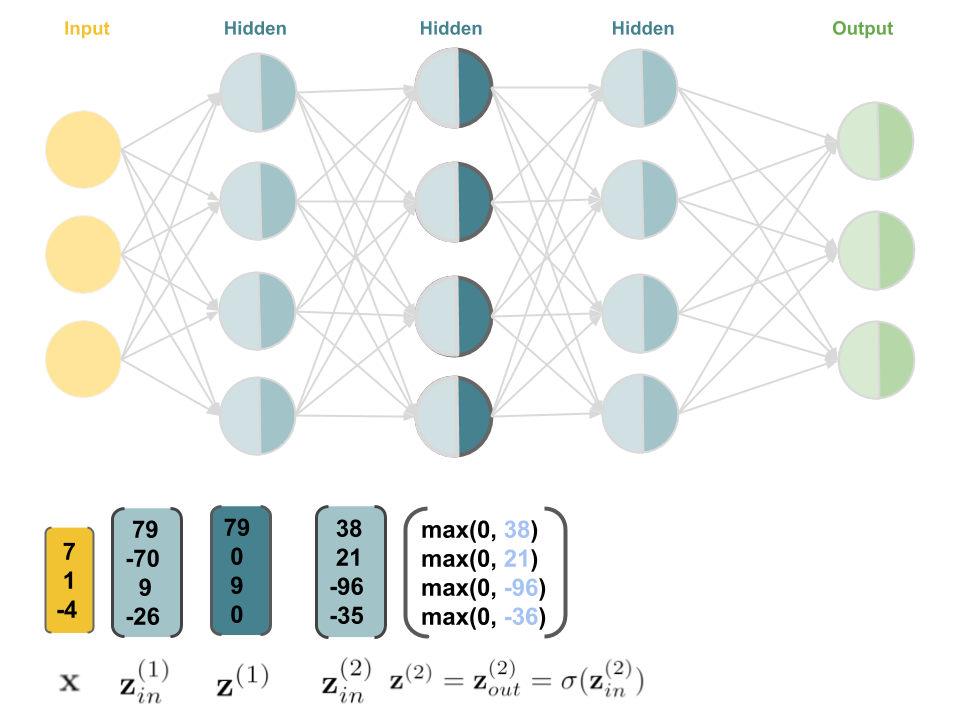
\includegraphics{figure/deepnet_six.png}}}
\only<7>{\scalebox{0.8}{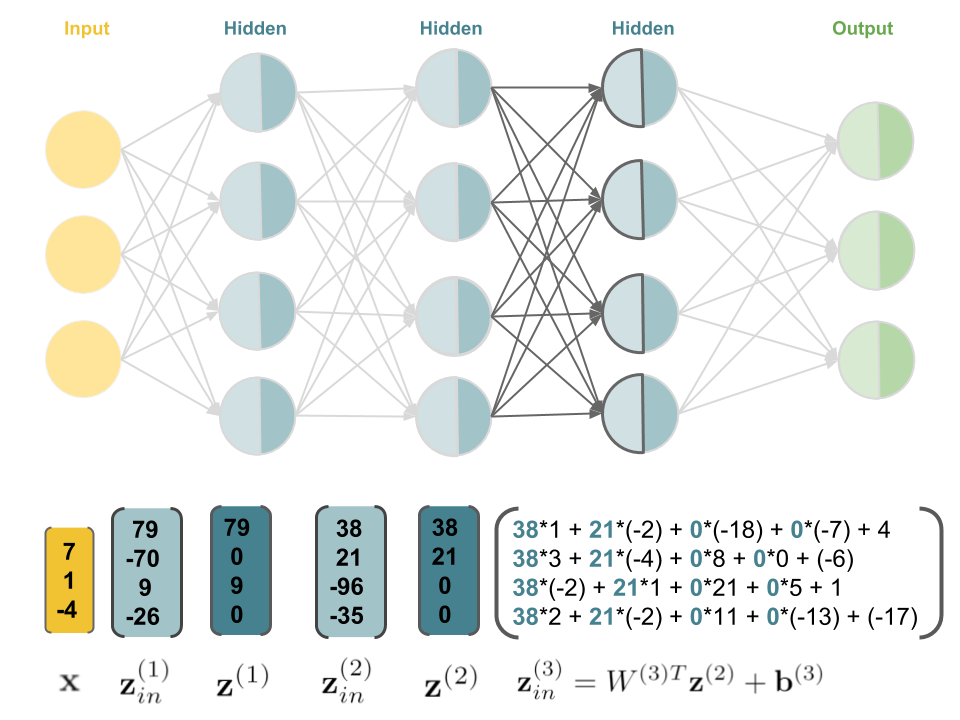
\includegraphics{figure/deepnet_seven.png}}}
\only<8>{\scalebox{0.8}{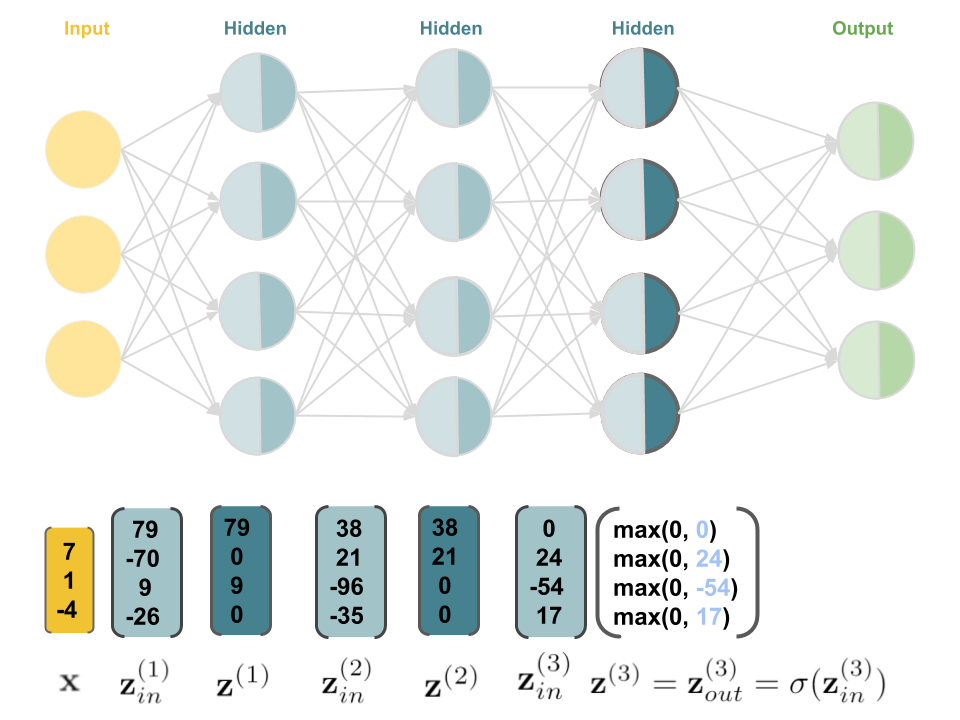
\includegraphics{figure/deepnet_eight.png}}}
\only<9>{\scalebox{0.8}{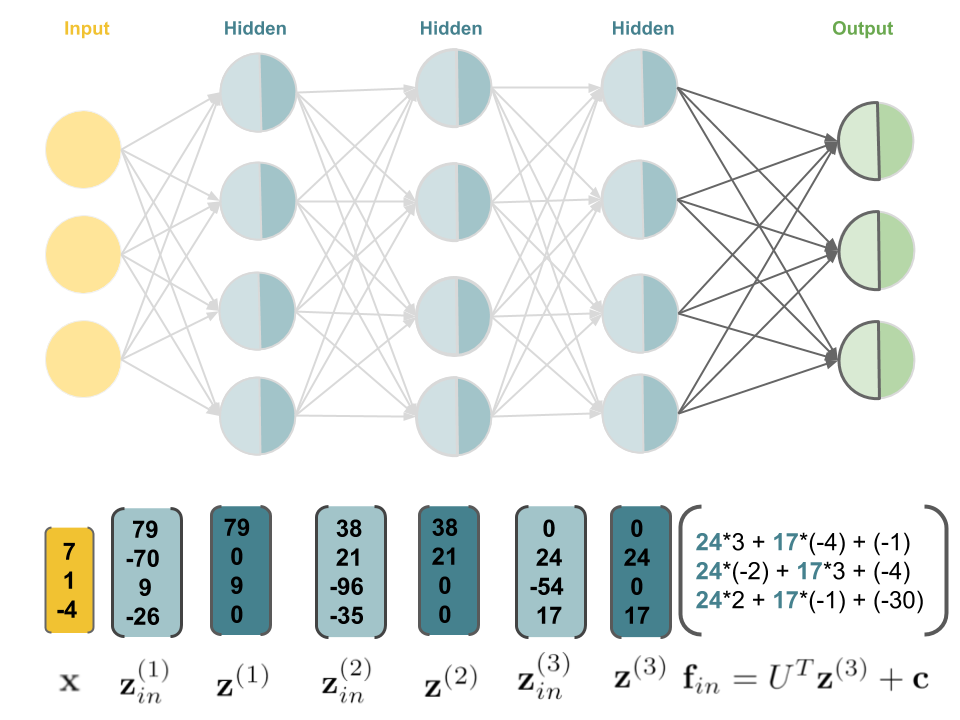
\includegraphics{figure/deepnet_nine.png}}}
\only<10>{\scalebox{0.8}{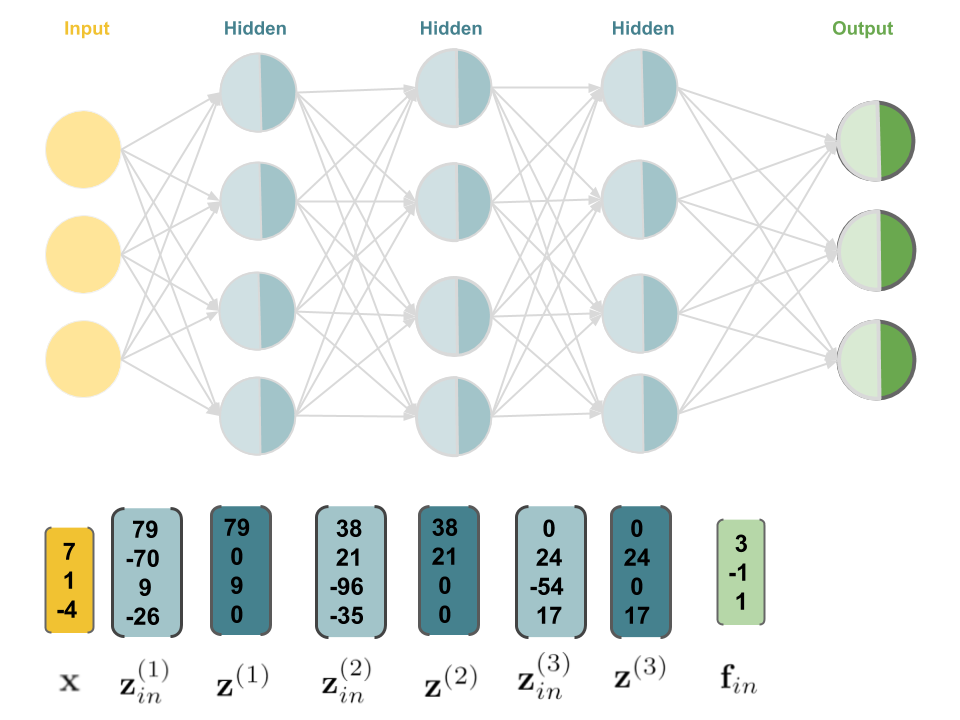
\includegraphics{figure/deepnet_ten.png}}}
\only<11>{\scalebox{0.8}{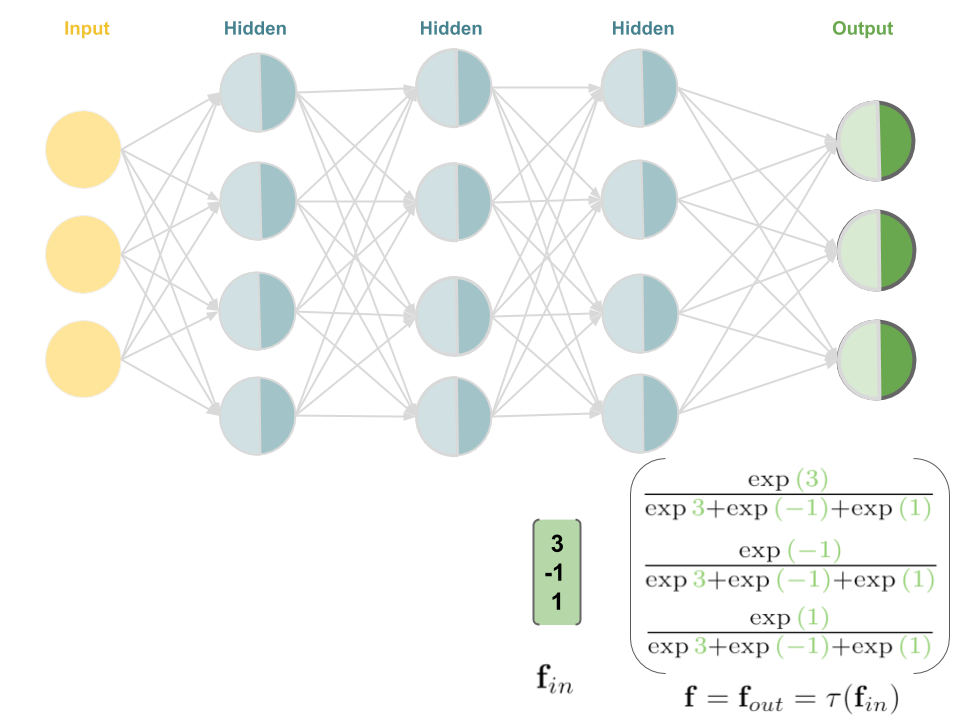
\includegraphics{figure/deepnet_eleven.png}}}
\only<12>{\scalebox{0.8}{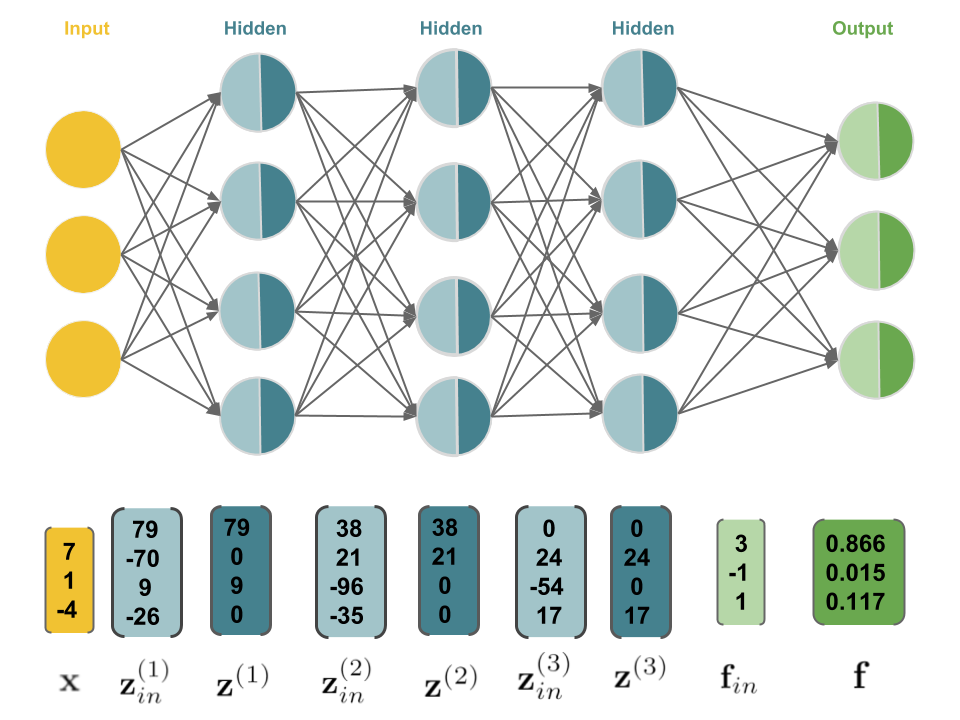
\includegraphics{figure/deepnet_twelve.png}}}
\end{figure}
\end{frame}
%%%%%%%%%%%%%%%%%%%%%%%%%%%%%%%%%%%%%%%%%%%%%%%%%%%%%%%%%%%%%%%%%%

\begin{vbframe}{Why add more layers?}
\begin{itemize}
\item Multiple layers allow for the extraction of more and more abstract
representations.
%\lz
\item Each layer in a feed-forward neural network adds its own degree of non-lnearity to the model.
\end{itemize}
%\lz
\begin{figure}
\centering
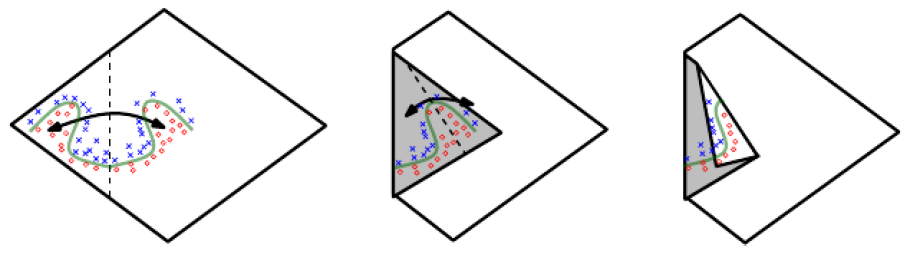
\includegraphics[width=10.5cm]{figure/folding}
\caption{An intuitive, geometric explanation of the exponential advantage of deeper networks formally (Mont\'{u}far et al., 2014).}
\end{figure}
\end{vbframe}
%%%%%%%%%%%%%%}%%%%%%%%%%%%%%%%%%%%%%%%%%%%%%%%%%%%%%%%%%%%%%%%%%%%%

\begin{vbframe}{Deep neural networks}

Neural networks today can have %dozens or even 
hundreds of hidden layers. The greater the number of layers, the "deeper" the network. Historically %, however, 
DNNs were very challenging to train and not popular until the late '00s for several reasons:
\lz
\begin{itemize}
\item %For one thing, the 
The use of sigmoid activations (e.g., logistic sigmoid and tanh) significantly slowed down training due to a phenomenon known as \enquote{vanishing gradients}. The introduction of the ReLU activation largely solved this problem.
\item Training DNNs on CPUs was too slow to be practical. Switching over to GPUs cut down training time by more than an order of magnitude.
\item When dataset sizes are small, other models (such as SVMs) and techniques (such as feature engineering) often outperform them. 
\end{itemize}
\framebreak
%%%%%%%%%%%%%%%%%%%%%%%%%%%%%%%%%%%%%%%%%%%%%%%%%%%%%%%%%%%%%%%%%%
\begin{itemize}
\item The availability of large datasets and novel architectures that are capable of handling even complex tensor-shaped data (e.g. CNNs for image data), faster hardware, and better optimization and regularization methods made it feasible to successfully implement deep neural networks.% in the last decade.
\lz

\item An increase in depth often translates to an increase in performance on a given task. State-of-the-art neural networks, however, are much more sophisticated than the simple architectures we have encountered so far.

\lz
%\item 
\end{itemize}
The term "\textbf{deep learning}" encompasses all of these developments and refers to the field as a whole.
\end{vbframe}
%%%%%%%%%%%%%%%%%%%%%%%%%%%%%%%%%%%%%%%%%%%%%%%%%%%%%%%%%%%%%%%%%%
%%%%%%%%%%%%%%%%%%%%%%%%%%%%%%%%%%%%%%%%%%%%%%%%%%%%%%%%%%%%%%%%%%
%%%%%%%%%%%%%%%%%%          REFERENCES          %%%%%%%%%%%%%%%%%%
%%%%%%%%%%%%%%%%%%%%%%%%%%%%%%%%%%%%%%%%%%%%%%%%%%%%%%%%%%%%%%%%%%
\begin{vbframe}
\frametitle{References}
\footnotesize{
\begin{thebibliography}{99}
%%%%%%%%%%%%%%%%%%%%%%%%%%%%%%%%%%
\bibitem[(Mont\'{u}far et al., 2014)]{1} Mont\'{u}farr, G., Pascanu, R., Cho, K., \& Bengio, Y. (2014). \textit{On the Number of Linear Regions of Deep Neural Networks}. 
\end{thebibliography}
}
\end{vbframe}

\section{Universal Approximation}

%\section{Universal Approximation}

\begin{vbframe}{Universal Approximation: What It Says}
\begin{itemize}
\item \textbf{Theorem (informal).} A neural network with a single hidden layer and enough hidden neurons can approximate any continuous function on a bounded input domain to arbitrary precision.
\vspace{4mm}
\item This holds for (almost) any non-linear activation function $\sigma$, and extends trivially to multiple outputs.
\vspace{4mm}
\item Two important caveats:
  \begin{itemize}
    \item The theorem only guarantees that suitable weights \textit{exist} --- not that training will find them.
    \vspace{2mm}
    \item \enquote{Enough hidden neurons} can mean an impractically large number: a network of fixed size can only represent a subspace of all continuous functions.
  \end{itemize}
\end{itemize}
\end{vbframe}
%%%%%%%%%%%%%%%%%%%%%%%%%%%%%%%%%%%%%%%%%%%%%%%%%%%%%%%%%%%%%%%%%%

\begin{vbframe}{Universal Approximation: The Catch}
\begin{itemize}
\item Universal approximation means approximation error can be driven to (near) zero --- so why not always use huge networks?
\vspace{4mm}
\item Because a highly flexible model class is also prone to \textbf{overfitting}: fitting the training data closely does not guarantee good generalization.
\vspace{4mm}
\item In practice, models of \textbf{intermediate flexibility} tend to generalize best; for neural networks, that means a reasonably (not maximally) sized hidden layer.
\vspace{4mm}
\item Let's see this in practice: decision boundaries learned by single-hidden-layer networks of different sizes, at different points during training.
\end{itemize}
\end{vbframe}
%%%%%%%%%%%%%%%%%%%%%%%%%%%%%%%%%%%%%%%%%%%%%%%%%%%%%%%%%%%%%%%%%%
\begin{frame}{Classification: 500 training iterations}

\only<1>{
\begin{knitrout}\scriptsize
\definecolor{shadecolor}{rgb}{0.969, 0.969, 0.969}\color{fgcolor}

{\centering 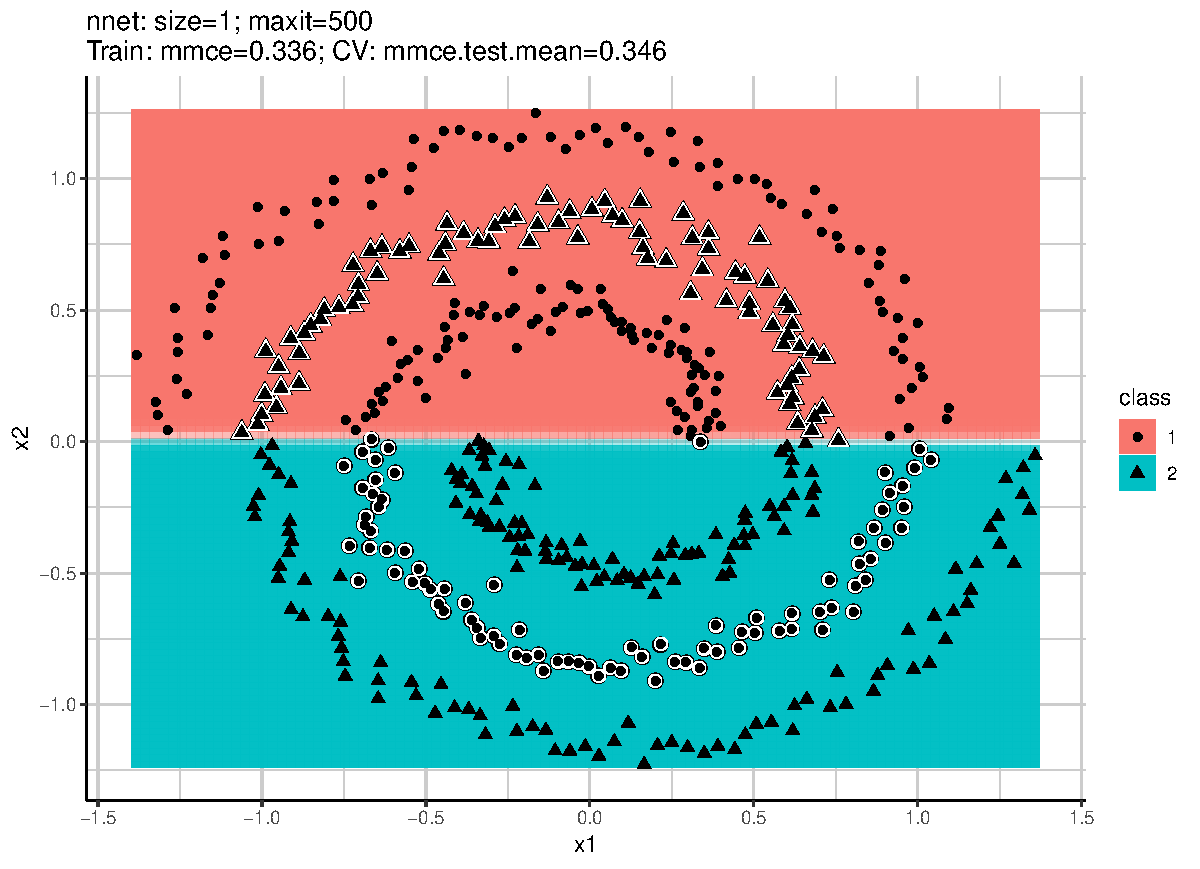
\includegraphics[width=0.72\textwidth]{figure/unnamed-chunk-6-1} 

}



\end{knitrout}
}

\only<2>{
\begin{knitrout}\scriptsize
\definecolor{shadecolor}{rgb}{0.969, 0.969, 0.969}\color{fgcolor}

{\centering 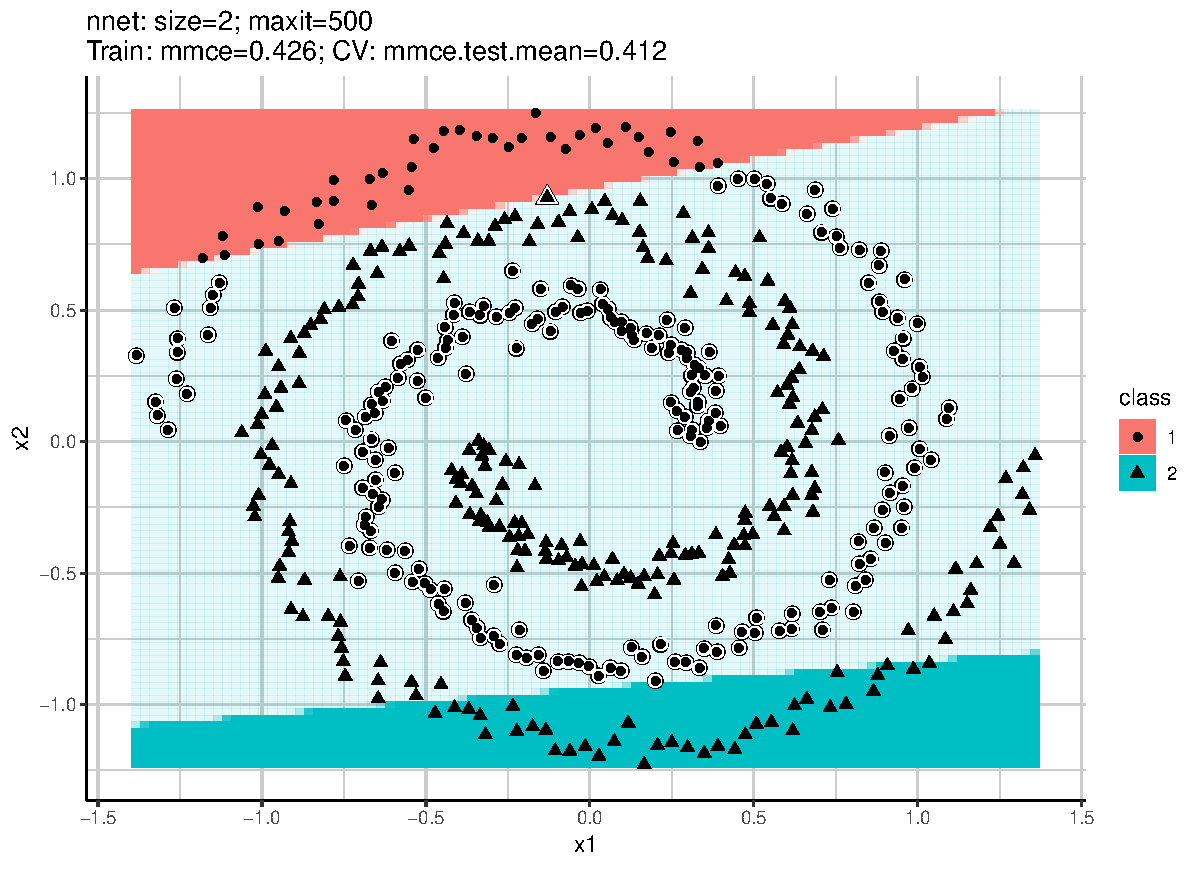
\includegraphics[width=0.72\textwidth]{figure/unnamed-chunk-7-1} 

}



\end{knitrout}
}

\only<3>{
\begin{knitrout}\scriptsize
\definecolor{shadecolor}{rgb}{0.969, 0.969, 0.969}\color{fgcolor}

{\centering 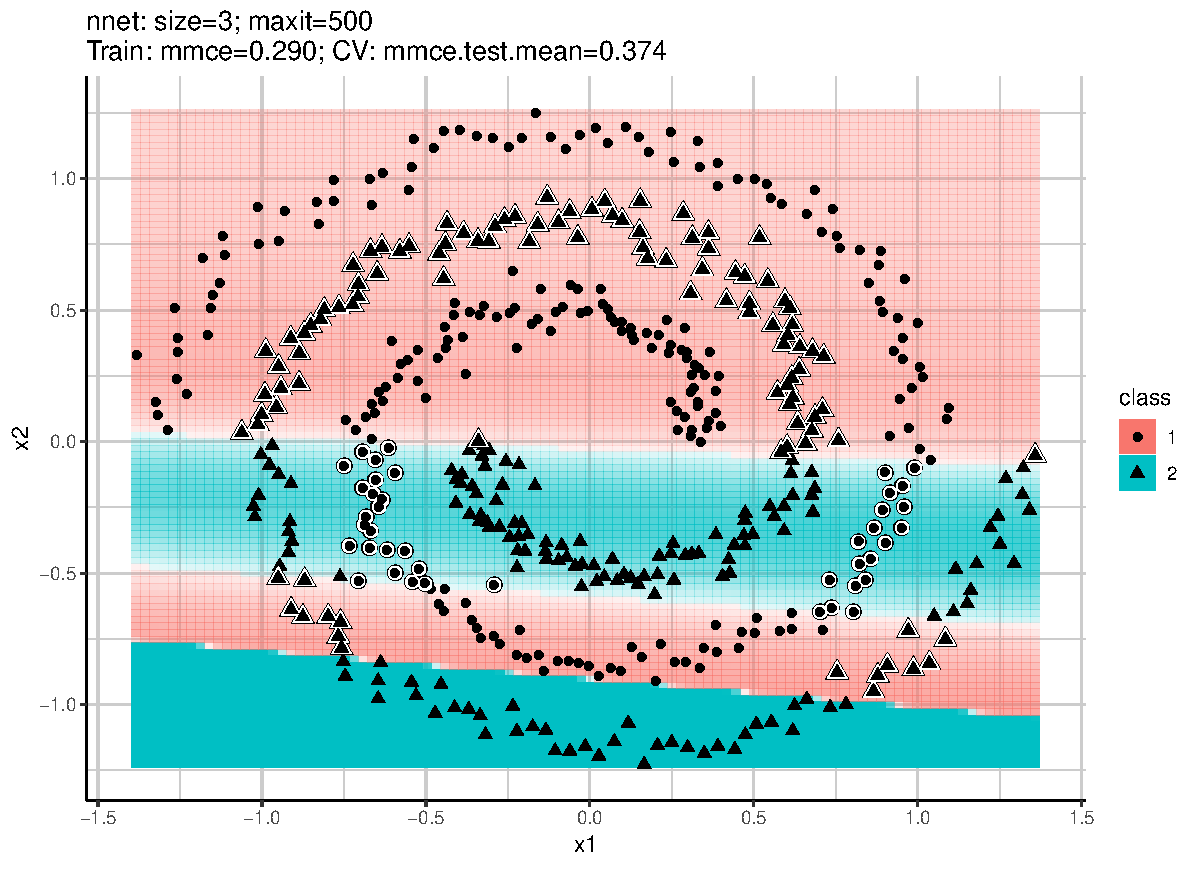
\includegraphics[width=0.72\textwidth]{figure/unnamed-chunk-8-1} 

}



\end{knitrout}
}

\only<4>{
\begin{knitrout}\scriptsize
\definecolor{shadecolor}{rgb}{0.969, 0.969, 0.969}\color{fgcolor}

{\centering 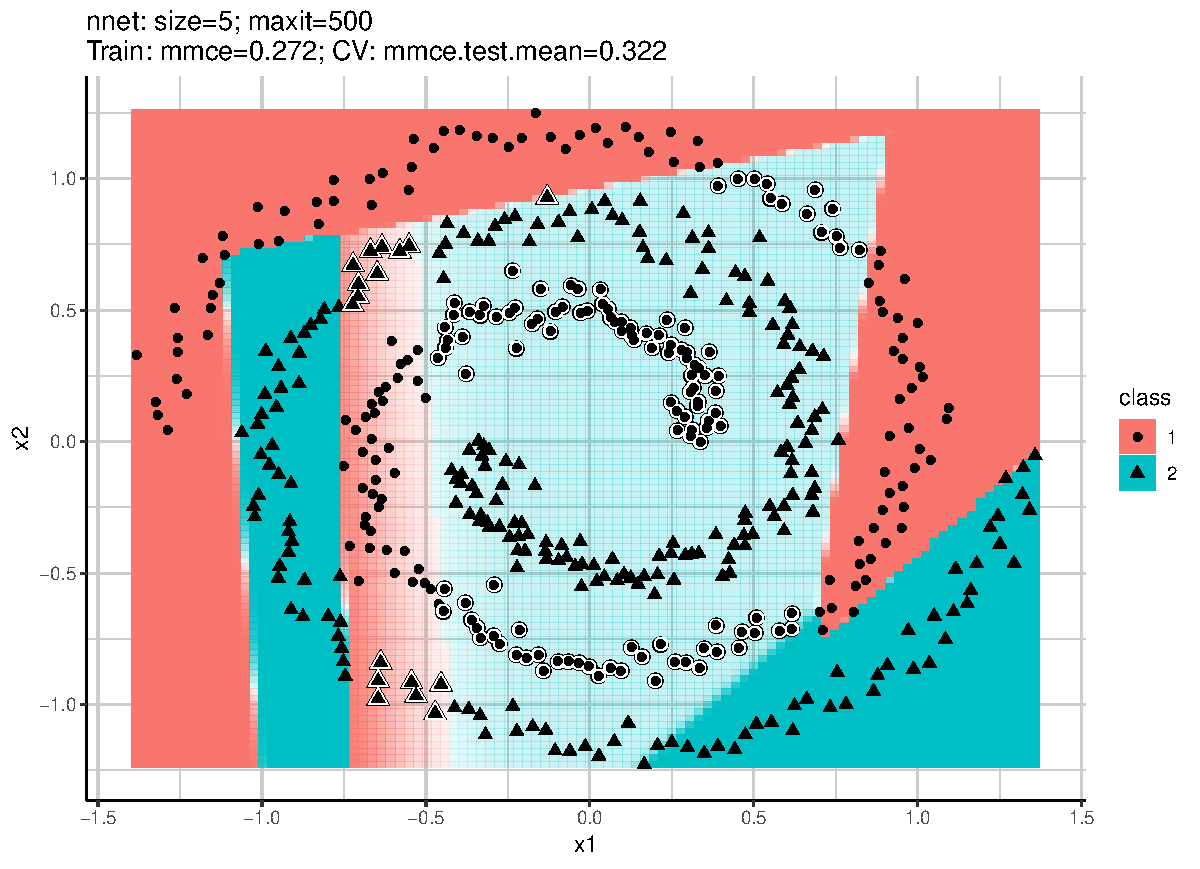
\includegraphics[width=0.72\textwidth]{figure/unnamed-chunk-9-1} 

}



\end{knitrout}
}

\only<5>{
\begin{knitrout}\scriptsize
\definecolor{shadecolor}{rgb}{0.969, 0.969, 0.969}\color{fgcolor}

{\centering 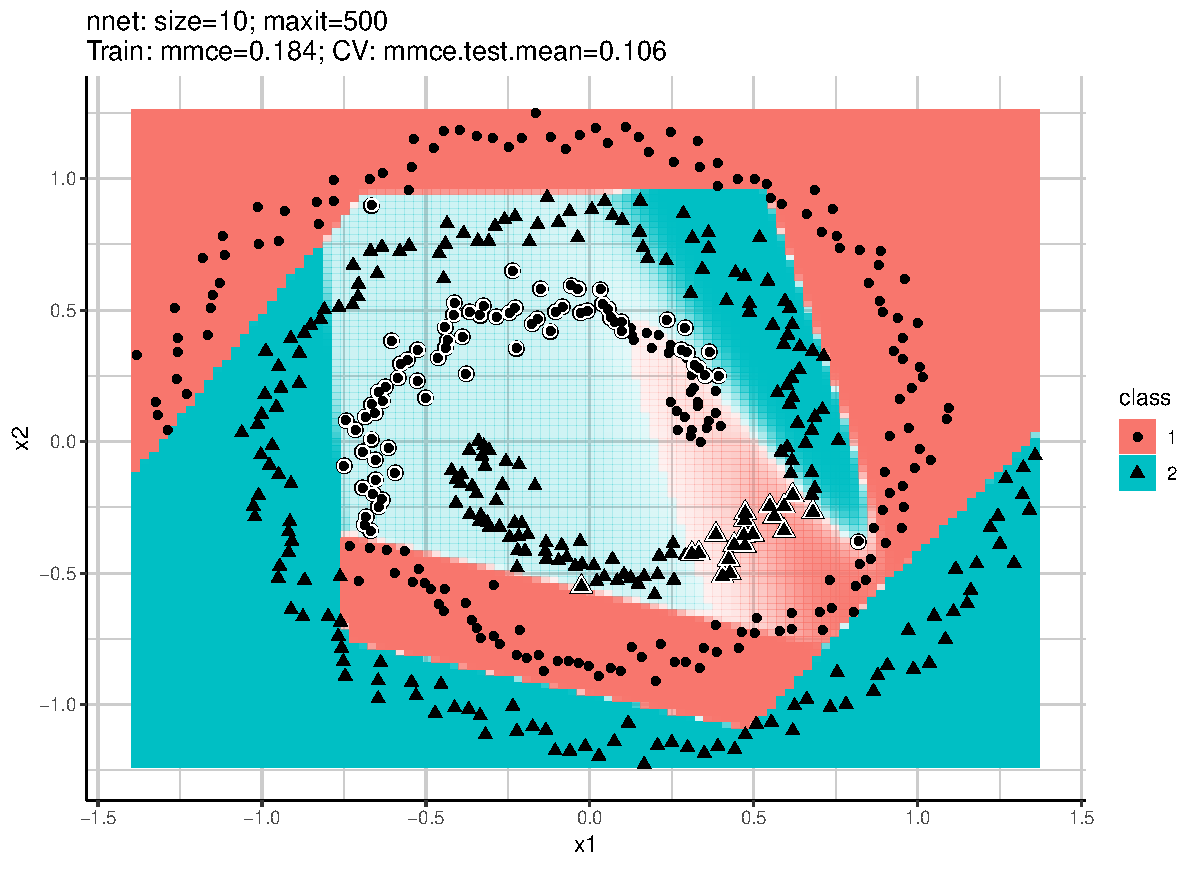
\includegraphics[width=0.72\textwidth]{figure/unnamed-chunk-10-1} 

}



\end{knitrout}
}

\only<6>{
\begin{knitrout}\scriptsize
\definecolor{shadecolor}{rgb}{0.969, 0.969, 0.969}\color{fgcolor}

{\centering 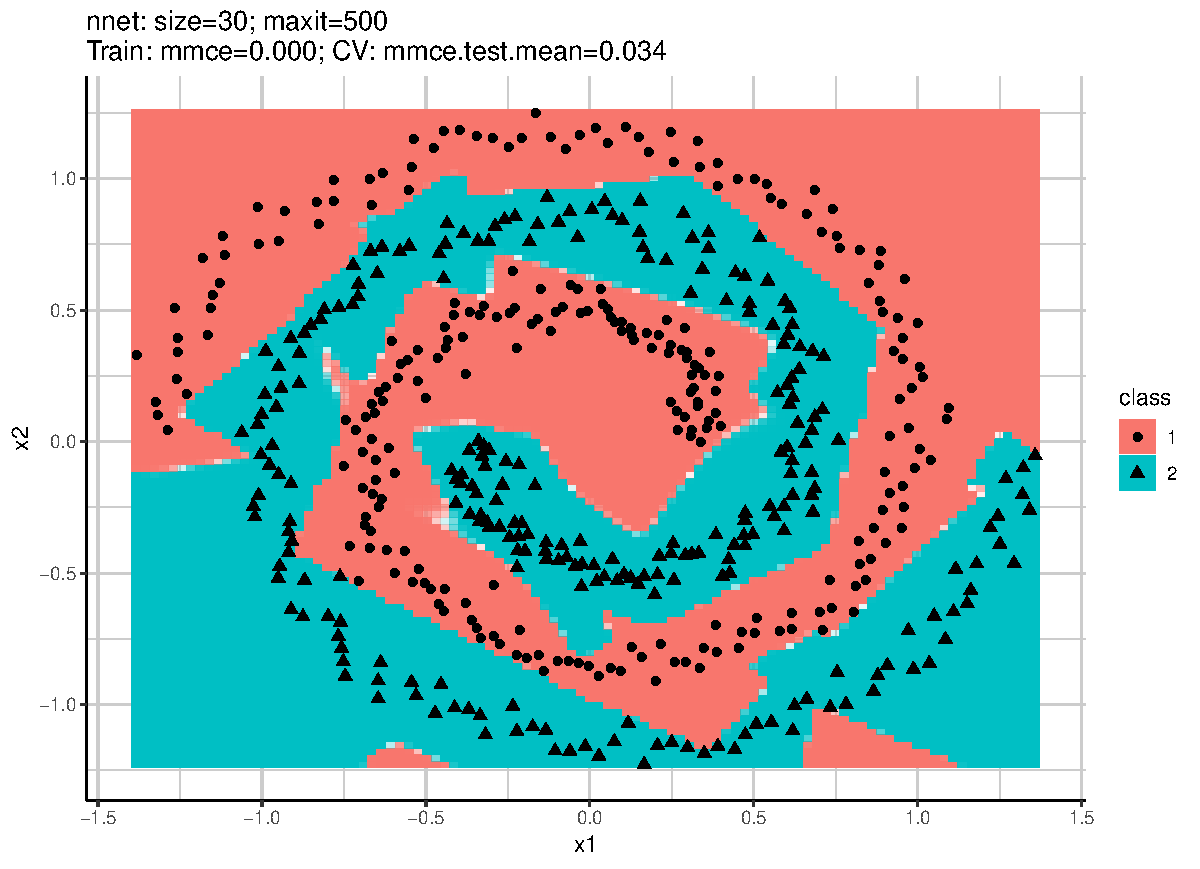
\includegraphics[width=0.72\textwidth]{figure/unnamed-chunk-11-1} 

}



\end{knitrout}
}

\only<7>{
\begin{knitrout}\scriptsize
\definecolor{shadecolor}{rgb}{0.969, 0.969, 0.969}\color{fgcolor}

{\centering 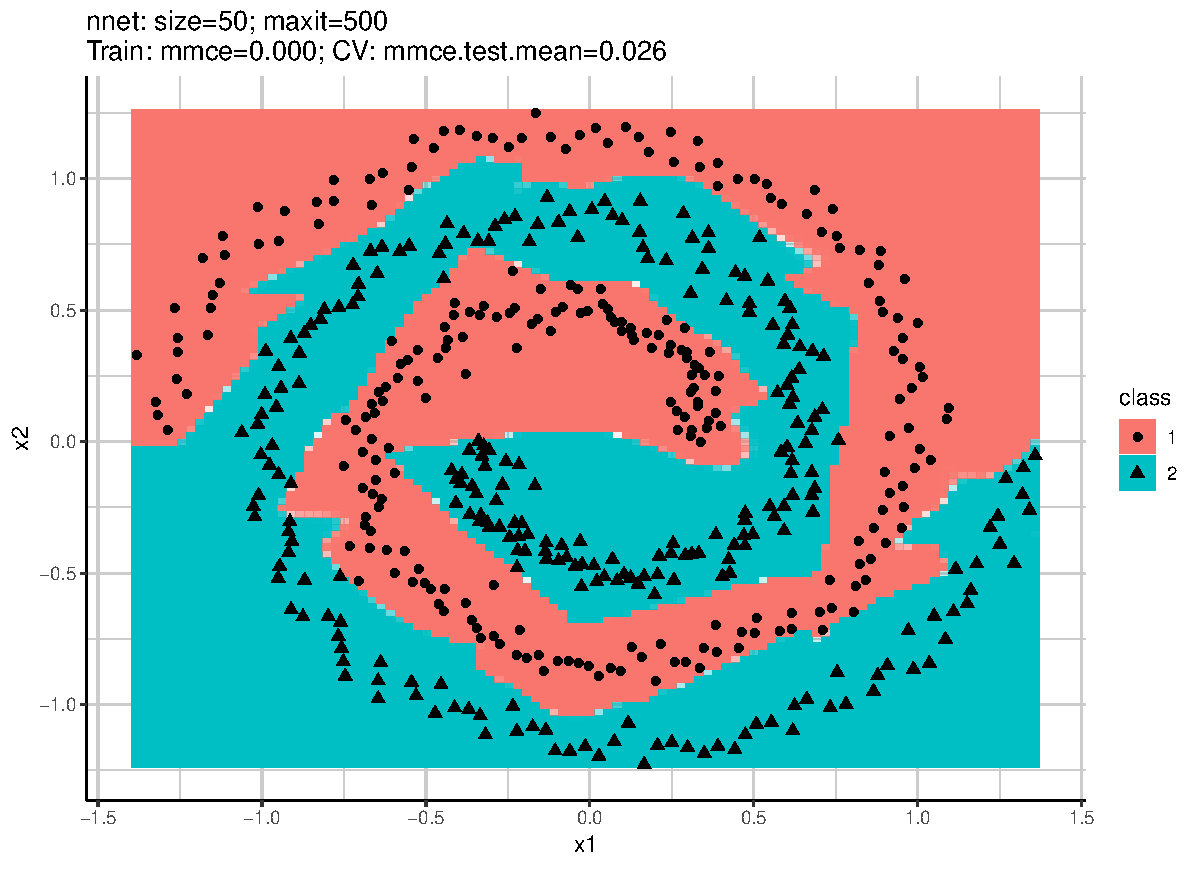
\includegraphics[width=0.72\textwidth]{figure/unnamed-chunk-12-1} 

}



\end{knitrout}
}

\end{frame}
%%%%%%%%%%%%%%%%%%%%%

\begin{vbframe}{License \& Attribution}
\begin{itemize}
\item This deck is adapted from \textbf{Introduction to Deep Learning (I2DL)},
Prof.\ Dr.\ Bernd Bischl, Statistical Learning and Data Science (SLDS),
LMU Munich. \url{https://github.com/slds-lmu/lecture_i2dl}
\item Licensed \textbf{CC BY 4.0}: \url{https://creativecommons.org/licenses/by/4.0/}
\item Content has been merged, reordered, and consolidated from the original
per-topic decks into this single session deck; not used verbatim.
\end{itemize}
\end{vbframe}

\endlecture
\end{document}
